% Aberdeen style guide should be followed when using this
% layout. Their template powerpoint slide is used to extract the
% Aberdeen color and logo but is otherwise ignored (it has little or
% no formatting in it anyway).
%
% http://www.abdn.ac.uk/documents/style-guide.pdf

%%%%%%%%%%%%%%%%%%%% Document Class Settings %%%%%%%%%%%%%%%%%%%%%%%%%
% Pick if you want slides, or draft slides (no animations)
%%%%%%%%%%%%%%%%%%%%%%%%%%%%%%%%%%%%%%%%%%%%%%%%%%%%%%%%%%%%%%%%%%%%%%
%Normal document mode
%\documentclass[10pt,compress]{beamer}
%Draft or handout mode
%\documentclass[10pt,compress,handout]{beamer}
\documentclass[10pt,compress,handout,ignorenonframetext]{beamer}
\newcommand{\frc}{\displaystyle\frac}


%%%%%%%%%%%%%%%%%%%% General Document settings %%%%%%%%%%%%%%%%%%%%%%%
% These settings must be set for each presentation
%%%%%%%%%%%%%%%%%%%%%%%%%%%%%%%%%%%%%%%%%%%%%%%%%%%%%%%%%%%%%%%%%%%%%%

\newcommand{\shortname}{Dr Jeff Gomes}
\newcommand{\fullname}{Dr Jeff Gomes}
\institute{School of Engineering}
\newcommand{\emailaddress}{jefferson.gomes@abdn.ac.uk}
\newcommand{\logoimage}{../FigBanner/UoAHorizBanner}
\title{Renewable Energy 1: Solar and Geothermal (EG501J)}
\subtitle{Module 3: Engineering Thermodynamics \\ (Heating and Refrigeration)}
\date[2014-15]{2014-15}

%%%%%%%%%%%%%%%%%%%% Template settings %%%%%%%%%%%%%%%%%%%%%%%%%%%%%%%
% You shouldn't have to change below this line, unless you want to.
%%%%%%%%%%%%%%%%%%%%%%%%%%%%%%%%%%%%%%%%%%%%%%%%%%%%%%%%%%%%%%%%%%%%%%
\usecolortheme{whale}
\useoutertheme{infolines}

% Use the fading effect for items that are covered on the current
% slide.
\beamertemplatetransparentcovered

% We abuse the author command to place all of the slide information on
% the title page.
\author[\shortname]{%
  \fullname\\\ttfamily{\emailaddress}
}


%At the start of every section, put a slide indicating the contents of the current section.
%\AtBeginSection[] {
%  \begin{frame}
%    \frametitle{Section Outline}
%    \tableofcontents[currentsection]
%  \end{frame}
%}

% Allow the inclusion of movies into the Presentation! At present,
% only the Okular program is capable of playing the movies *IN* the
% presentation.
\usepackage{multimedia}
\usepackage{animate}
\usepackage{comment} 

%%%%% Color settings
\usepackage{color}
%% The background color for code listings (i.e. example programs)
\definecolor{lbcolor}{rgb}{0.9,0.9,0.9}%
\definecolor{UoARed}{rgb}{0.64706, 0.0, 0.12941}
\definecolor{UoALight}{rgb}{0.85, 0.85, 0.85}
\definecolor{UoALighter}{rgb}{0.92, 0.92, 0.92}
\setbeamercolor{structure}{fg=UoARed} % General background and higlight color
\setbeamercolor{frametitle}{bg=black} % General color
\setbeamercolor{frametitle right}{bg=black} % General color
\setbeamercolor{block body}{bg=UoALighter} % For blocks
\setbeamercolor{structure}{bg=UoALight} % For blocks
% Rounded boxes for blocks
\setbeamertemplate{blocks}[rounded]

%%%%% Font settings
% Aberdeen requires the use of Arial in slides. We can use the
% Helvetica font as its widely available like so
% \usepackage{helvet}
% \renewcommand{\familydefault}{\sfdefault}
% But beamer already uses a sans font, so we will stick with that.

% The size of the font used for the code listings.
\newcommand{\goodsize}{\fontsize{6}{7}\selectfont}

% Extra math packages, symbols and colors. If you're using Latex you
% must be using it for formatting the math!
\usepackage{amscd,amssymb} \usepackage{amsfonts}
\usepackage[mathscr]{eucal} \usepackage{mathrsfs}
\usepackage{latexsym} \usepackage{amsmath} \usepackage{bm}
\usepackage{amsthm} \usepackage{textcomp} \usepackage{eurosym}
% This package provides \cancel{a} and \cancelto{a}{b} to "cancel"
% expressions in math.
\usepackage{cancel}

% Get rid of font warnings as modern LaTaX installations have scalable
% fonts
\usepackage{type1cm} 

%\usepackage{enumitem} % continuous numbering throughout enumerate commands

% For exact placement of images/text on the cover page
\usepackage[absolute]{textpos}
\setlength{\TPHorizModule}{1mm}%sets the textpos unit
\setlength{\TPVertModule}{\TPHorizModule} 

% Source code formatting package
\usepackage{listings}%
\lstset{ backgroundcolor=\color{lbcolor}, tabsize=4,
  numberstyle=\tiny, rulecolor=, language=C++, basicstyle=\goodsize,
  upquote=true, aboveskip={1.5\baselineskip}, columns=fixed,
  showstringspaces=false, extendedchars=true, breaklines=false,
  prebreak = \raisebox{0ex}[0ex][0ex]{\ensuremath{\hookleftarrow}},
  frame=single, showtabs=false, showspaces=false,
  showstringspaces=false, identifierstyle=\ttfamily,
  keywordstyle=\color[rgb]{0,0,1},
  commentstyle=\color[rgb]{0.133,0.545,0.133},
  stringstyle=\color[rgb]{0.627,0.126,0.941}}

% Allows the inclusion of other PDF's into the final PDF. Great for
% attaching tutorial sheets etc.
\usepackage{pdfpages}
\setbeamercolor{background canvas}{bg=}  

% Remove foot note horizontal rules, they occupy too much space on the slide
\renewcommand{\footnoterule}{}

% Force the driver to fix the colors on PDF's which include mixed
% colorspaces and transparency.
\pdfpageattr {/Group << /S /Transparency /I true /CS /DeviceRGB>>}

% Include a graphics, reserve space for it but
% show it on the next frame.
% Parameters:
% #1 Which slide you want it on
% #2 Previous slides
% #3 Options to \includegraphics (optional)
% #4 Name of graphic
\newcommand{\reserveandshow}[4]{%
\phantom{\includegraphics<#2|handout:0>[#3]{#4}}%
\includegraphics<#1>[#3]{#4}%
}


\begin{document}

% Title page layout
\begin{frame}
  \titlepage
  \vfill%
  \begin{center}
    \includegraphics[clip,width=0.8\textwidth]{\logoimage}
  \end{center}
\end{frame}


%%%
%%% Summary 
%%%
\begin{frame}
\frametitle{Overview} % Table of contents slide, comment this block out to remove it
\tableofcontents % Throughout your presentation, if you choose to use \section{} and \subsection{} commands, these will automatically be printed on this slide as an overview of your presentation
\end{frame}



%%%%%%%%%%%%%%%%%%%% The Presentation Proper %%%%%%%%%%%%%%%%%%%%%%%%%
% Fill below this line with \begin{frame} commands! It's best to
% always add the fragile option incase you're going to use the
% verbatim environment.
%%%%%%%%%%%%%%%%%%%%%%%%%%%%%%%%%%%%%%%%%%%%%%%%%%%%%%%%%%%%%%%%%%%%%%


%%%           %%%
%%%  SECTION  %%% 
%%%           %%%
\section{Introduction}

%%%
%%% Slide
%%%
\begin{frame}
 \frametitle{Overview}
  \begin{enumerate}[(a)]
   \item <1-> The \textcolor{blue}{red}{First Law} stated the equivalence between the quantity of heat used and the mechanical work but;
   \item <2-> It does not specify the conditions in which the conversion -- \textcolor{blue}{heat $\Leftrightarrow$ work} -- may occur and;
   \item <3-> The direction in which heat transfer may take place;
   \item <4-> This led to both the concept of \textcolor{blue}{irreversibility} and the \textcolor{red}{Second Law}.
   \item <5-> If we consider a heat engine running thermodynamically backward, it becomes a heat pump, a refrigerator or an air conditioner;
   \item <6-> Thus the objective of a \textcolor{red}{refrigeration process} \textcolor{blue}{is to keep a cold body at a temperature below the temperature of the surroundings by the removal of heat from the system}.
   %\item <6-> 
  \end{enumerate}
\end{frame}


%%%
%%% Slide
%%%
\begin{frame}
 \frametitle{Overview}
  \begin{columns}
   \begin{column}[c]{0.45\linewidth}
    \begin{enumerate}[(a)] \setcounter{enumi}{6}
     \item <1-> When a heat engine is thermodynamically reversed, the \textcolor{blue}{directions of all the energy flows are reversed};
     \item <2-> Work input ({\it W}) causes thermal energy transfers $Q_{2}$ from the cold reservoir and $Q_{1}=Q_{2}+W$ to the hot reservoir; 
     \item <3-> Such reversed process can not however occur spontaneously. The transfer of heat from a cold reservoir to a hot reservoir requires special devices called \textcolor{blue}{refrigerators}.
    \end{enumerate}
   \end{column}
   \begin{column}[c]{0.55\linewidth}
    \begin{figure}%
     \begin{center}
      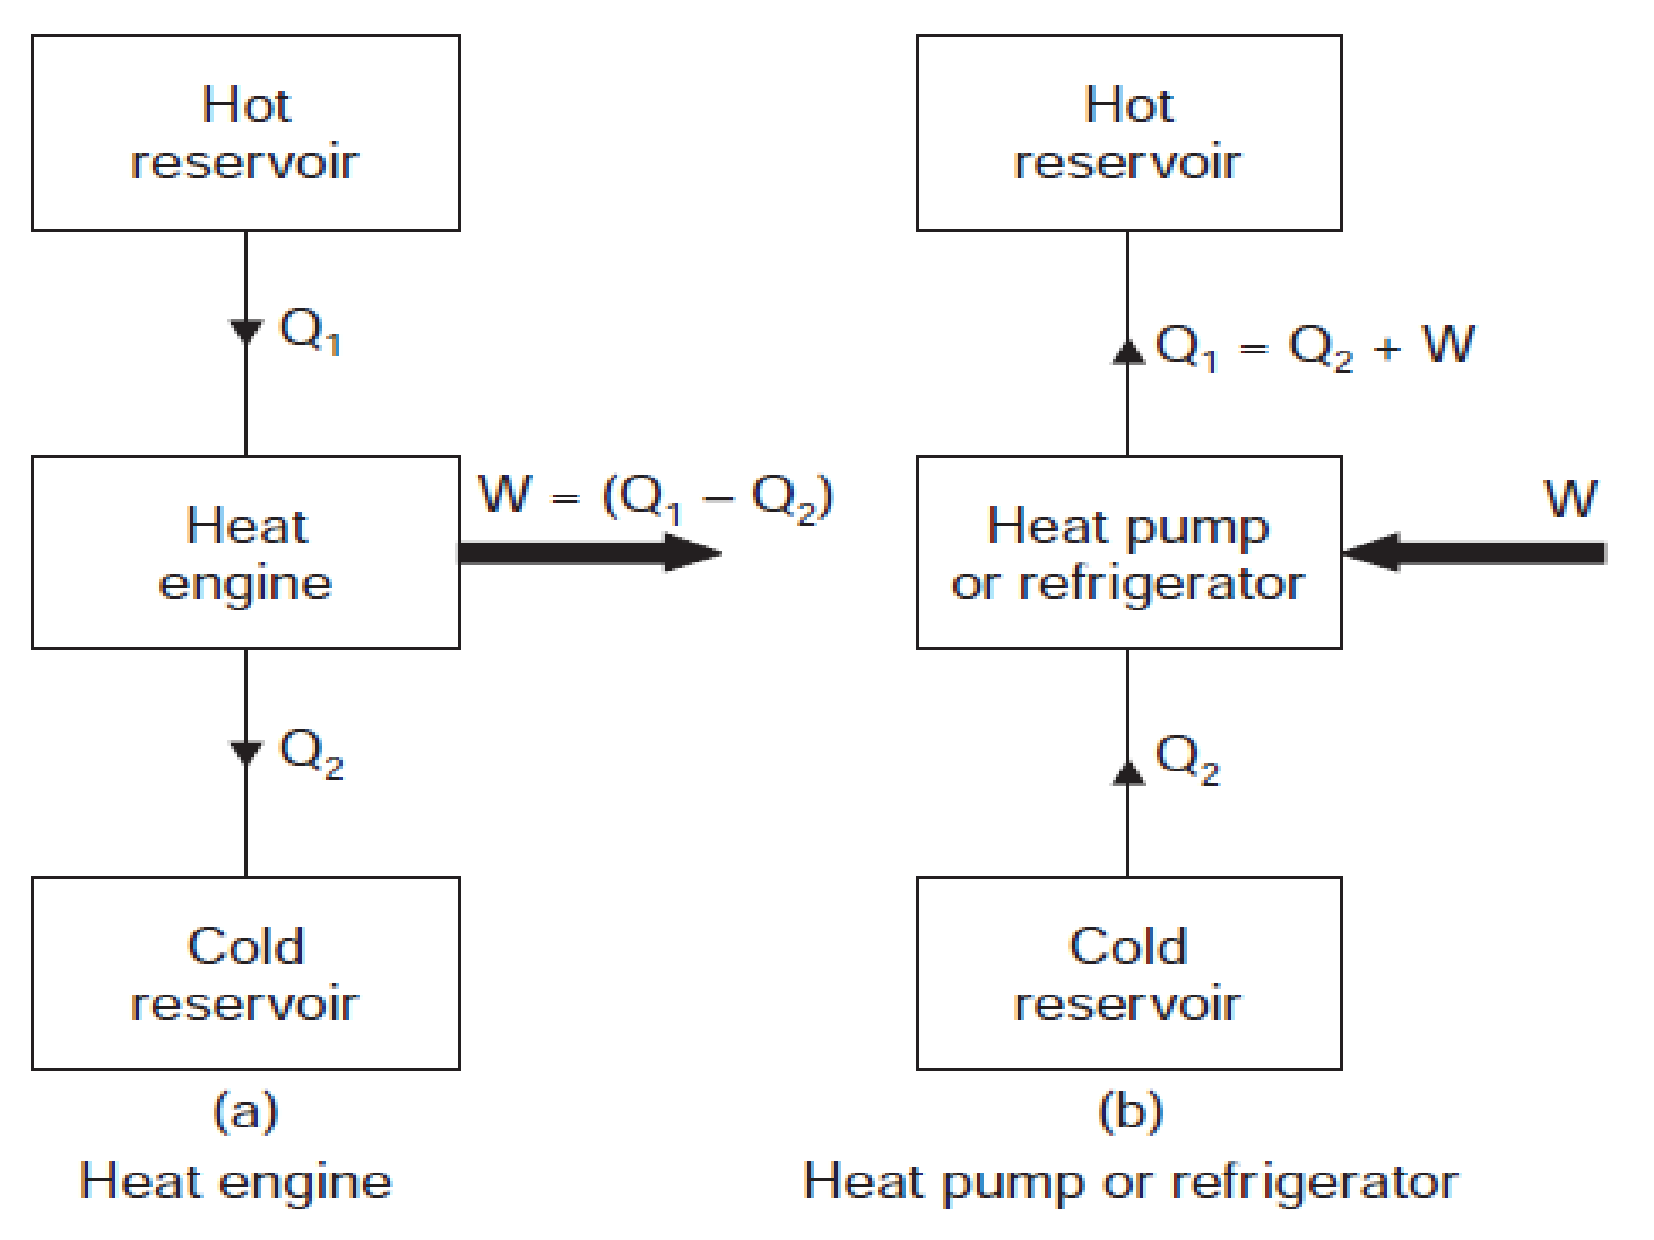
\includegraphics[width=6.5cm,clip]{./Pics/Overview_Refrig1}
     \end{center}
    \end{figure}  
   \end{column}  
  \end{columns}
\end{frame}



\section{Bibliography} 
%%%
%%% Slide
%%%
\begin{frame}
 \frametitle{Suggested References}
  Literature relevant for this module:
  \begin{enumerate}[(a)]
   \item J.M. Smith, H.C. Van Ness and M.M. Abbott, $\lq$Introduction to Chemical Engineering Thermodynamics', 6$^{th}$ Edition: Chapters 9.1-.3, 9.5;
   \item I. Muller and W.H. Muller, $\lq$Fundamentals of Thermodynamics and Applications' (2009): Chapters 6.3;
   \item Y.A. Cengel and M.A. Boles, $\lq$Thermodynamics -- An Engineering Approach' , 5$^{th}$ Edition: Chapters 11.1-5, 11.7-8;
   \item E. Logan, $\lq$Thermodynamics -- Processes and Applications' (1999): 8.1-4;
   \item R.T. Balmer, $\lq$Modern Engineering Thermodynamics' (2011) Chapters: 14.2,5-9;
   \item \href{http://www.sfsb.unios.hr/test/testhome/vtAnimations/animations/chapter09/refrigeration/index1.html}{\tiny{http://www.sfsb.unios.hr/test/testhome/vtAnimations/animations/chapter09/refrigeration/index1.html}}
  \end{enumerate}
\end{frame}



%%%
%%% SECTION
%%%
\section{Refrigerator and Heat Pump}

\subsection{Definitions}

%%%
%%% Slide
%%%
\begin{frame}
 \frametitle{Refrigerator and Heat Pump}
  \begin{columns}
   \begin{column}[c]{0.45\linewidth}
     \begin{enumerate}[(a)]
     \item <1-> \textcolor{blue}{Refrigerators} are cyclic devices, and the working fluids are called \textcolor{blue}{refrigerants};
     \item <2-> In the refrigerator, \textcolor{red}{$Q_{L}$} represents the \textcolor{blue}{heat removed} from the cold reservoir at temperature \textcolor{red}{$T_{L}$} whereas;
     \item <3-> \textcolor{red}{$Q_{H}$} is the \textcolor{blue}{heat rejected} to the hot reservoir at temperature \textcolor{red}{$T_{H}$} and 
     \item <4-> \textcolor{red}{$W_{\text{net}}$} is the \textcolor{blue}{net work input} to the refrigerator;
     \item <5-> {\bf \textcolor{blue}{Refrigerator} and \textcolor{red}{Heat Pump} are similar devices in which the only difference is their objectives};
    \end{enumerate}
   \end{column}
   \begin{column}[c]{0.55\linewidth}
    \begin{figure}%
     \begin{center}
      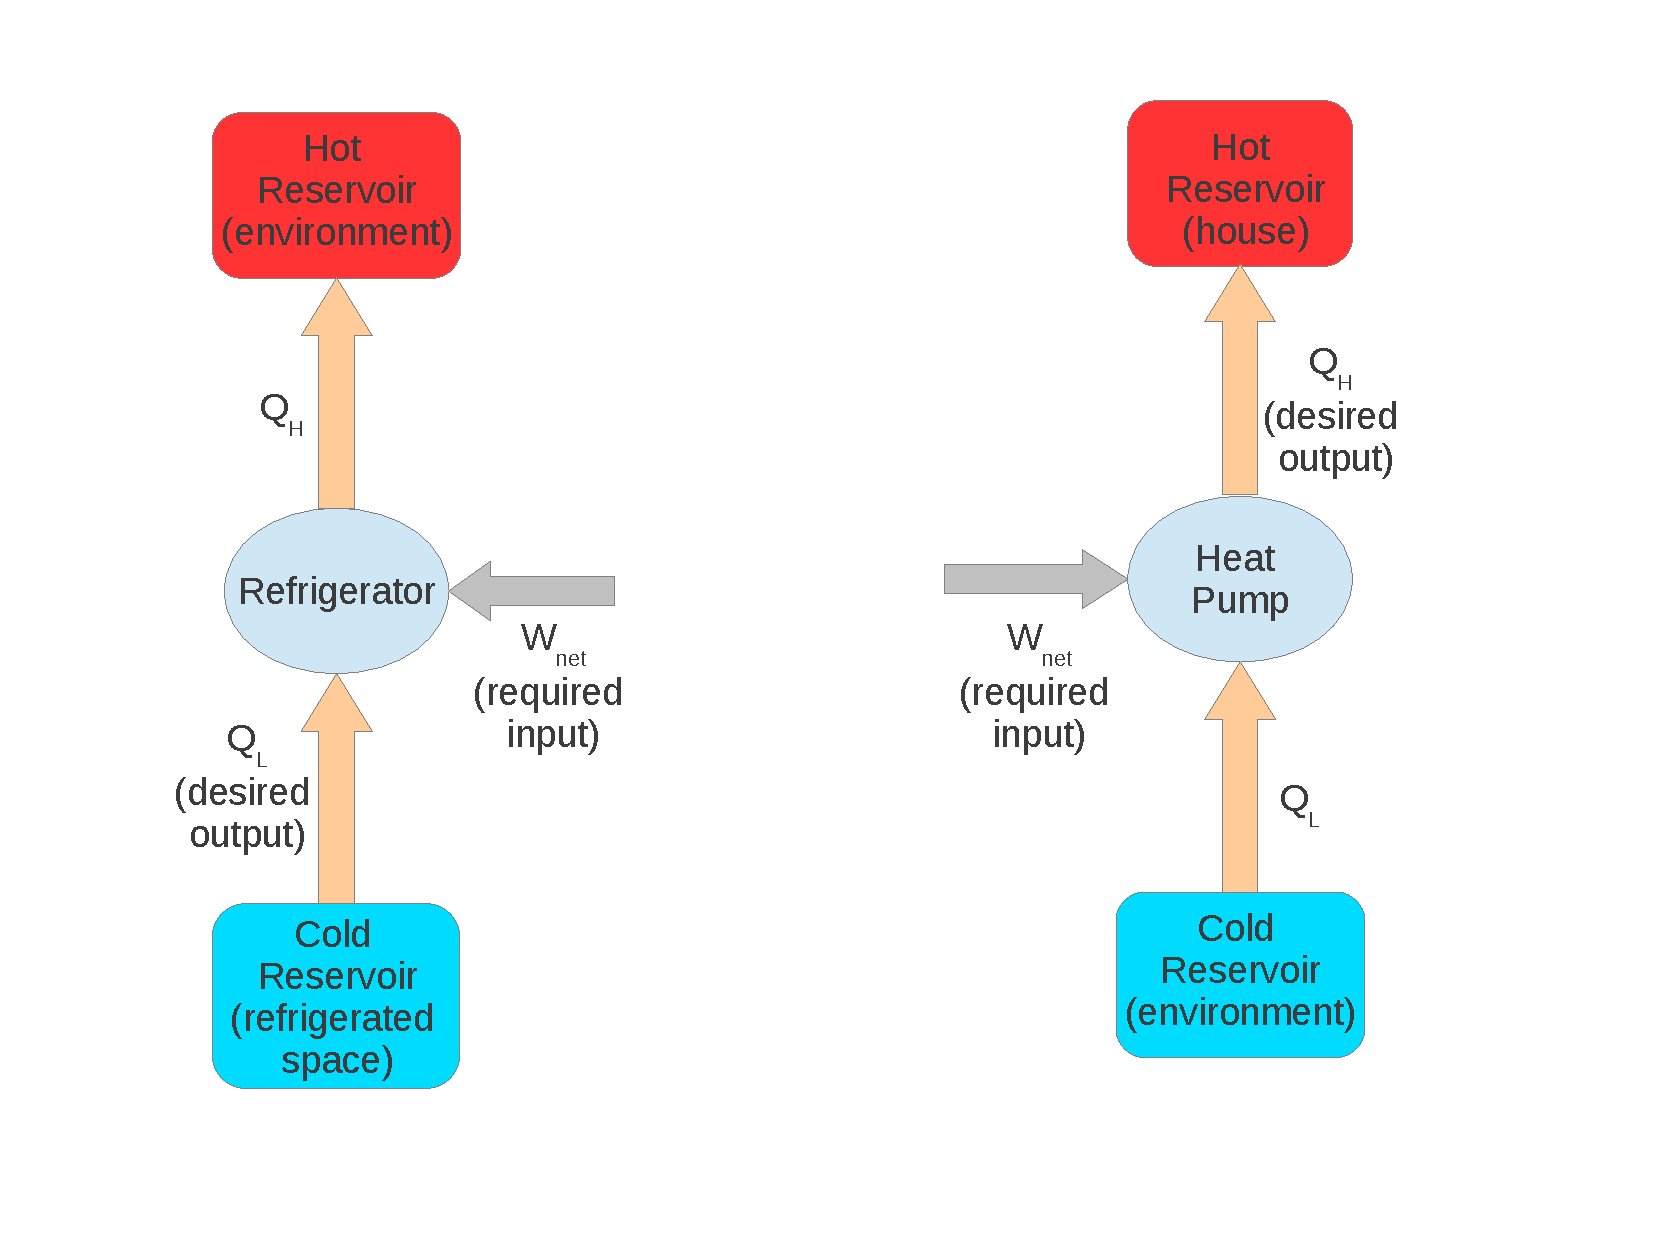
\includegraphics[width=7.5cm,clip]{./Pics/Overview_Refrig2}
     \end{center}
    \end{figure}
   \end{column}  
  \end{columns}
\end{frame}

%%%
%%% Slide
%%%
\begin{frame}
 \frametitle{}
  \begin{columns}
   \begin{column}[c]{0.45\linewidth}
    \begin{enumerate}\setcounter{enumi}{6}
     \item <1-> A \textcolor{blue}{Refrigerator} aims to keep the cold reservoir at $T_{L}$ by removing heat from it;
     \item <2-> Discharging the heat to a hot reservoir operating at $T_{H}$ is part of the operation not the objective.
     \item <3-> \textcolor{blue}{Heat Pump} aims to maintain a heated space at a high temperature $T_{H}$ by;
     \item <4-> Absorbing heat from a cold reservoir (low-temperature source, e.g., well water of cold outside air during winter) and supplying this heat to a warmer reservoir.
    \end{enumerate}
   \end{column}
   \begin{column}[c]{0.55\linewidth}
    \begin{figure}%
     \begin{center}
      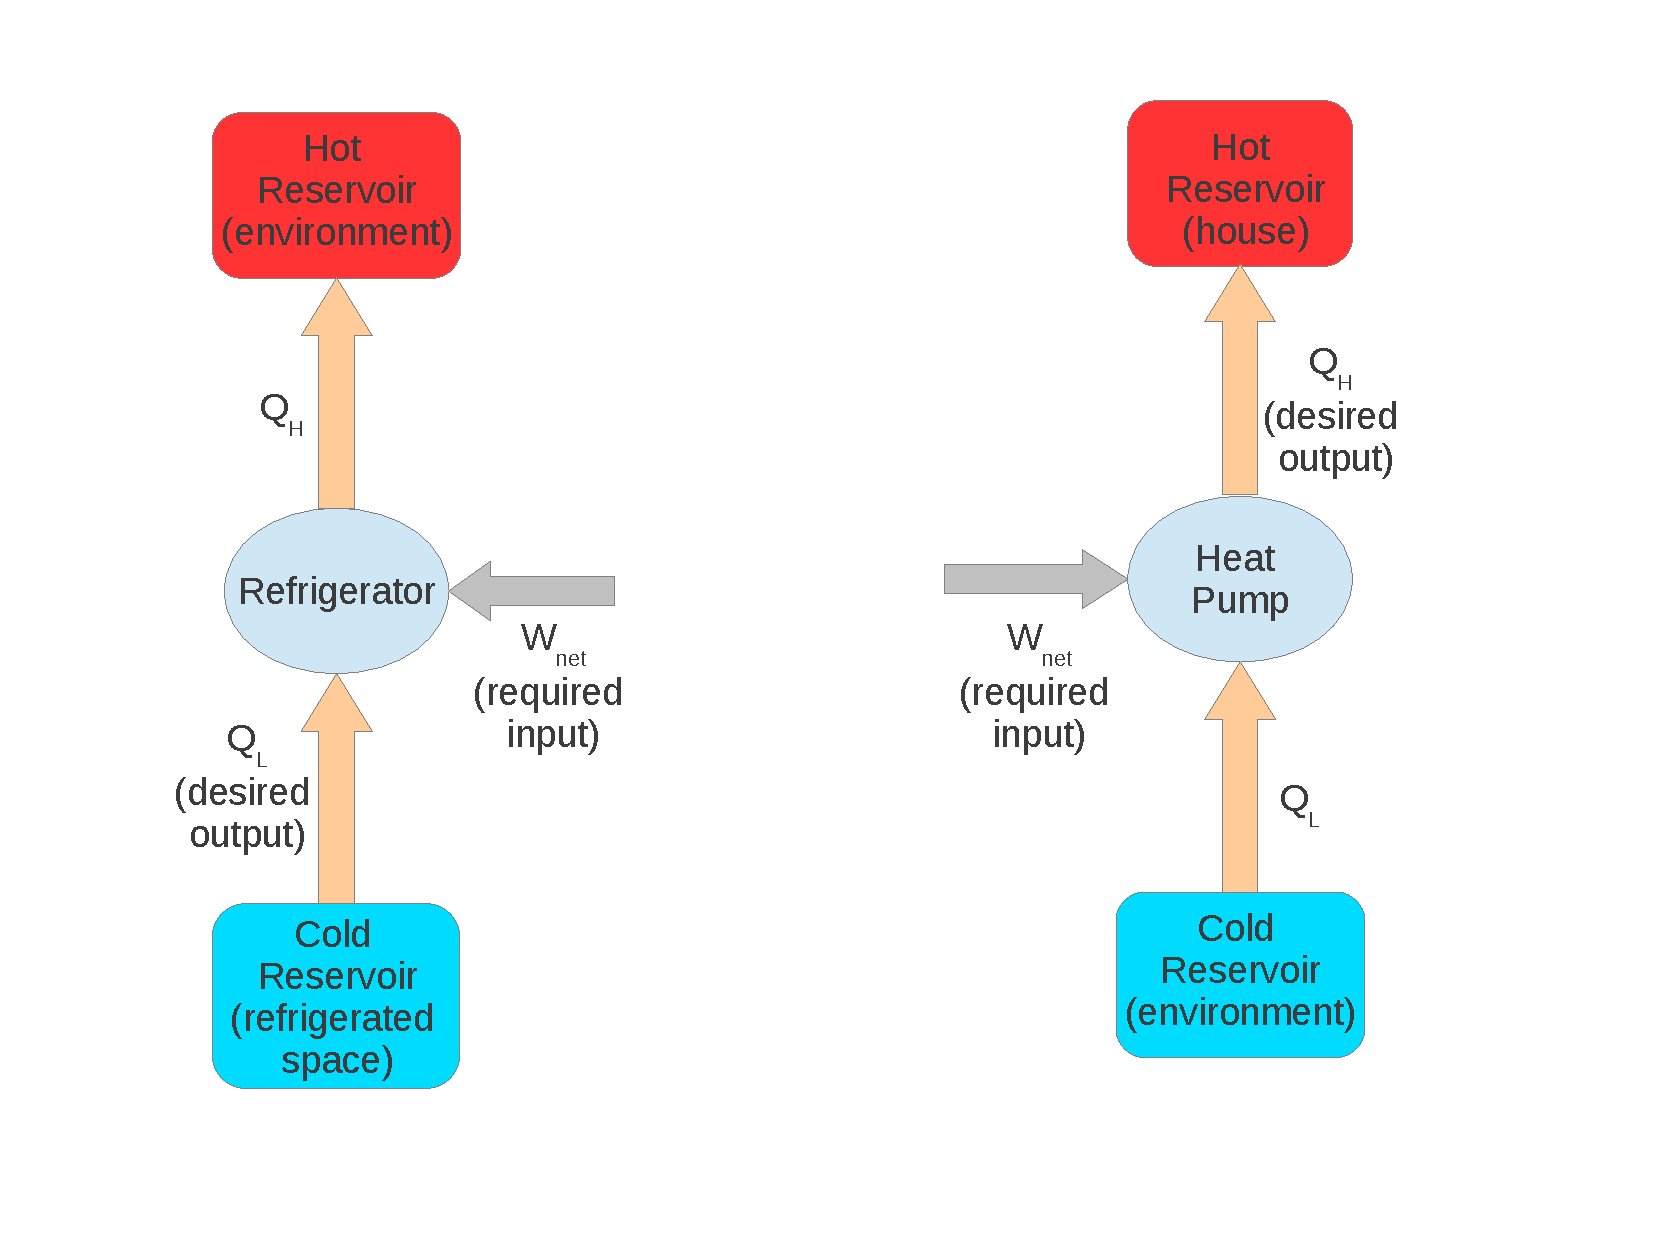
\includegraphics[width=7.5cm,clip]{./Pics/Overview_Refrig2}
     \end{center}
    \end{figure}  
   \end{column}  
  \end{columns}
\end{frame}

%%%
%%% Slide
%%%
\begin{frame}
 \frametitle{Refrigerator and Heat Pump}
    \begin{figure}%
     \begin{center}
      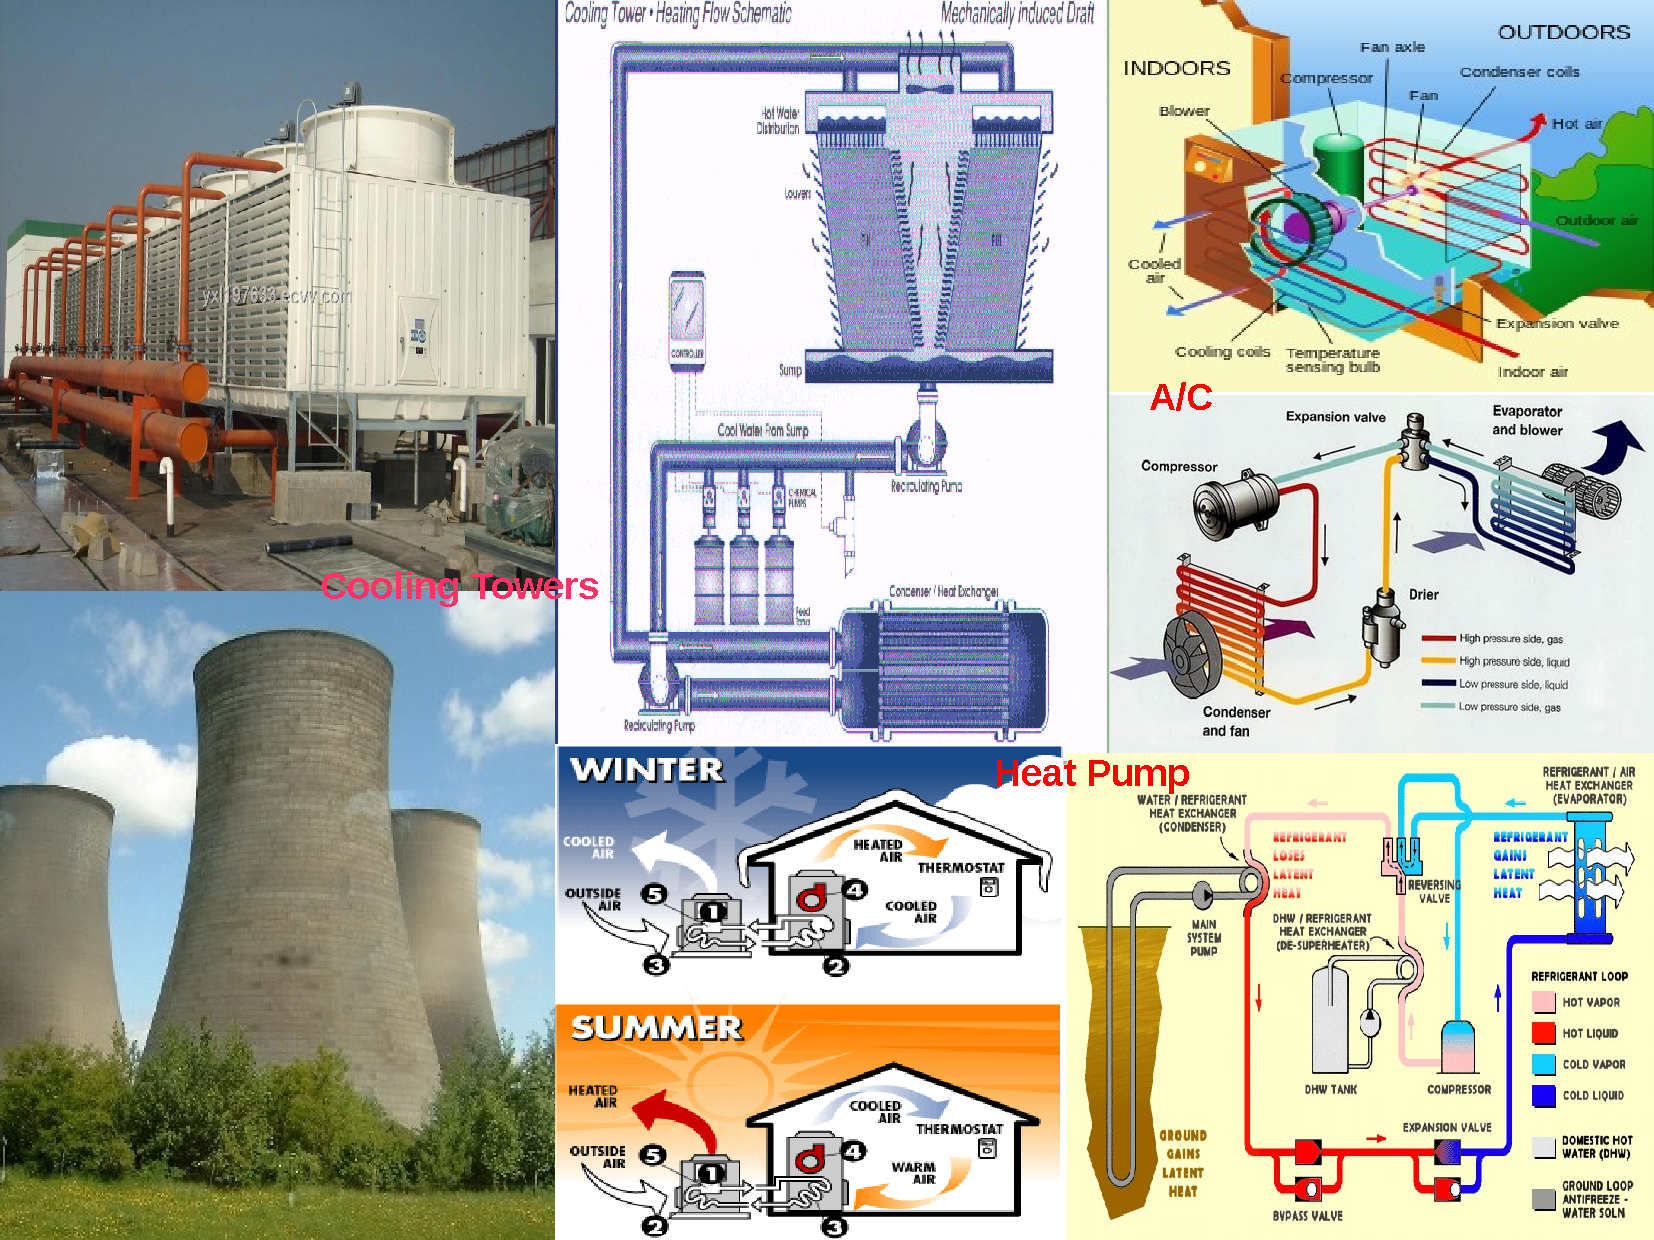
\includegraphics[width=12.cm,height=7.8cm]{./Pics/Overview_Refrig3}
     \end{center}
    \end{figure}
\end{frame}


%%%
%%% Slide
%%%
\begin{frame}
 \frametitle{Coefficient of Performance (COP)}
 \begin{itemize}
  \item <1-> COP is the ratio of heat absorbed by the refrigerant while passing through the evaporator to the work input required to compress the refrigerant in the compressor;
   \textcolor{blue}{
   \begin{eqnarray}
    \text{COP}_{R} &=&\frc{\text{Desired Output}}{\text{Required Input}}=\frc{\text{Cooling Effect}}{\text{Work Input}}=\frc{Q_{L}}{W_{net,in}} \nonumber\\
                   &=& \frc{Q_{L}}{|Q_{H}|-Q_{L}}\label{Ref1:1}
   \end{eqnarray}
   \begin{eqnarray}
   \text{COP}_{HP}&=&\frc{\text{Desired Output}}{\text{Required Input}}=\frc{\text{Heating Effect}}{\text{Work Input}}=\frc{Q_{H}}{W_{net,in}} \nonumber \\
                 &=&\frc{Q_{H}}{|Q_{H}|-Q_{L}}    \label{Ref1:2}
   \end{eqnarray}}
  \item <2-> In other words, it is the ratio between heat extracted and work done;
  \item <3-> For fixed $Q_{L}$ and $Q_{H}$, Eqns. \ref{Ref1:1} and \ref{Ref1:2} lead to \textcolor{blue}{$\text{COP}_{HP}=\text{COP}_{R}+1$}.
  \item <4->This means that \textcolor{blue}{COP$_{HP}>1$} and, obviously \textcolor{red}{COP$_{R}$ is positive}.
 \end{itemize}
\end{frame}

%%%
%%% Slide
%%%
\begin{frame}
 \frametitle{Coefficient of Performance (COP)}
 \begin{itemize}
  \item <1-> We should recall the Carnot thermal efficiency, $\eta_{T}=1-\frc{|Q_{L}|}{Q_{H}}$;
  \item <2-> Thus,
   \begin{equation}
    \text{COP}_{HP}=\frc{1}{\eta_{T}}\;\;\;\text{ and }\;\;\;\text{COP}_{R}=\frc{1}{\eta_{T}}-1
     \label{Ref1:3}
   \end{equation}
  \item <3-> We can then conclude that the {\it COP} for any heat engine operating on a reversed thermodynamic cycle (e.g., heat pump or refrigerator) could also be obtained from Eqn. \ref{Ref1:3}. 
  \item <4-> As the Carnot thermal efficiency can also be expressed as a function of the temperature of the hot and cold reservoirs, $\eta_{T}^{\text{Carnot}}=1-\frc{T_{L}}{T_{H}}=\frc{T_{H}-T_{L}}{T_{L}}$, the {\it COP} for Carnot engine running backwards can also be expressed as,
\begin{equation}
\text{COP}_{HP}^{\text{Carnot}}=\frc{T_{H}}{T_{H}-T_{L}}\;\;\;\text{ and }\;\;\; \text{COP}_{R}^{\text{Carnot}}=\frc{T_{L}}{T_{H}-T_{L}}
\end{equation}
 \end{itemize}
\end{frame}

\subsection{Unit of Refrigeration}
%%%
%%% Slide
%%%
\begin{frame}
 \frametitle{Unit of Refrigeration (Tonne)}
 \begin{itemize}
  \item <1-> \textcolor{blue}{Refrigeration effect is the amount of heat extracted by the refrigerator from the refrigerated space.}
  \item <2-> This effect is quantified by the \textcolor{blue}{unit of refrigeration}, or \textcolor{red}{Ton of refrigeration};
  \item <3-> \textcolor{red}{One Ton (or Tonne)} of refrigeration is defined as the amount of heat removed from one ton of water at 0$^{\text{o}}$C to form 1 ton of ice within 24 hours, thus;
  \item <4-> A \textcolor{red}{Ton of refrigeration} quantifies the latent heat $\left(L_{f}\right)$ required to be removed for solidification of water at 0$^{\text{o}}$C, i.e.,
  %\item \textcolor{red}{1 Ton of Refrigeration} = {\it mass of water} $\times$ {\it Latent Heat of fusion at 0$^{\text{o}}C$ from water liquid to ice};
   \begin{eqnarray}
    \textcolor{red}{\text{1 Ton of Refrigeration}} &=& \text{mass of water} \times L_{f} \nonumber \\
                                                   &=& \textcolor{red}{3.5\;\;\text{kJ/s}} \simeq \textcolor{blue}{200\;\; \text{Btu/min}}\nonumber 
   \end{eqnarray}
 \end{itemize}
\end{frame}




\section{Reversed Carnot Cycle for Refrigeration}
%%%
%%% Slide
%%%
\begin{frame}
 \frametitle{Reversed Carnot Cycle}
  \begin{columns}
   \begin{column}[c]{0.45\linewidth}
    \begin{itemize}
     \item <1-> As we saw before, Carnot cycle is the most efficient and ideal thermal cycle and can also be used to get refrigerant effect upon its reversal;
     \item <2-> Refrigerated body needs to be kept at low temperature $T_{L}=T_{2}$ for which heat $\left(Q_{L}\right)$ should be removed at constant rate;
     \item <3-> Rejected to surroundings at high temperature, $T_{H}=T_{1}$;
     \item <4-> The amount of heat rejected to the surroundings is Q$_{H}$ while the net work done is {\it W};
    \end{itemize}
   \end{column}
   \begin{column}[c]{0.55\linewidth}
    \begin{figure}%
     \begin{center}
      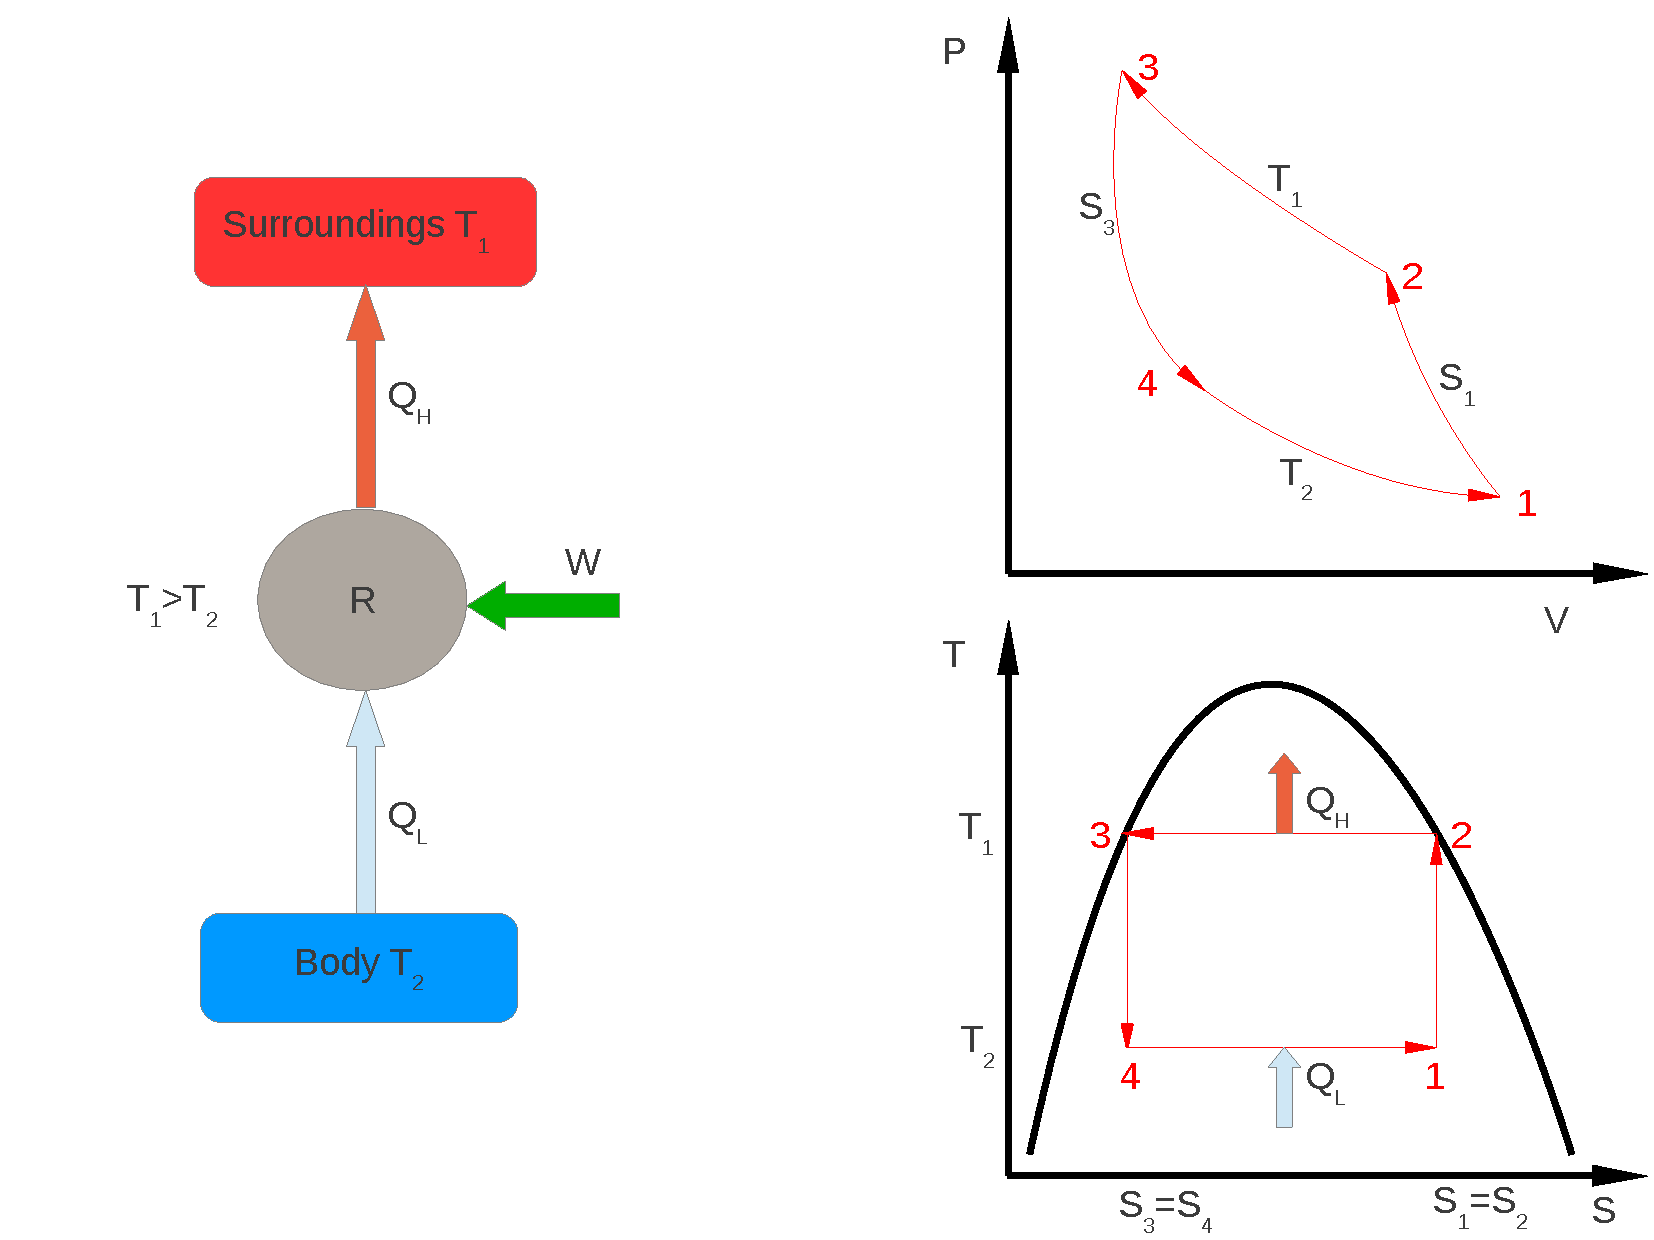
\includegraphics[width=6.8cm,height=6.5cm]{./Pics/Overview_Refrig4}
     \end{center}
    \end{figure}  
   \end{column}  
  \end{columns}
\end{frame}




%%%
%%% Slide
%%%
\begin{frame}
 \frametitle{Reversed Carnot Cycle}
  \begin{columns}

   \begin{column}[c]{0.55\linewidth}
    \begin{figure}%
     \begin{center}
      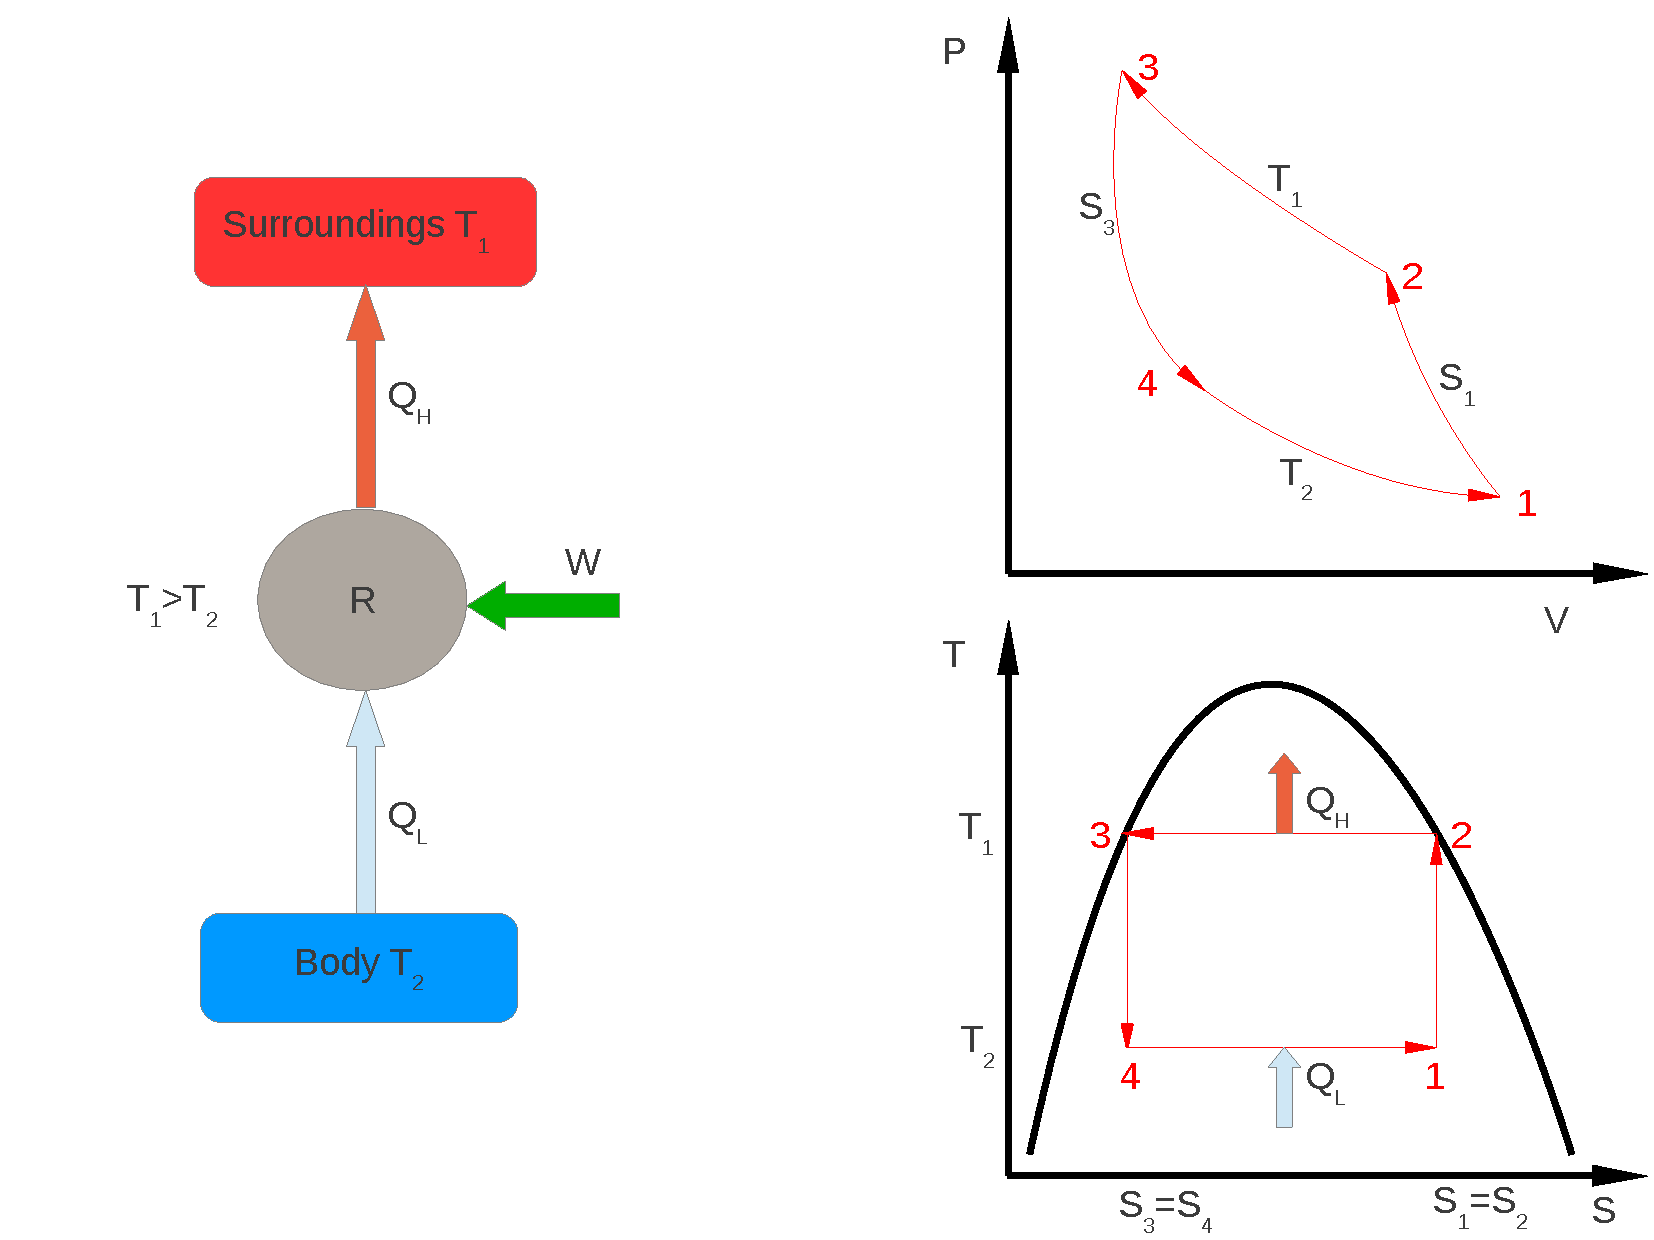
\includegraphics[width=6.8cm,height=6.cm]{./Pics/Overview_Refrig4}
     \end{center}
    \end{figure}  
   \end{column}  


   \begin{column}[c]{0.45\linewidth}
    The four stages are:
    \begin{enumerate}[(a)]
     \item <1-> \textcolor{red}{1--2:} Reversible adiabatic compression;
     \item <2-> \textcolor{red}{2--3:} Reversible isothermal heat rejection $\left(Q_{H}\right)$ at $T_{1}$;
     \item <3-> \textcolor{red}{3--4:} Reversible adiabatic expansion;
     \item <4-> \textcolor{red}{4--1:} Reversible isothermal heat absorption $\left(Q_{L}\right)$ at $T_{2}$;
    \end{enumerate}
   \end{column}
  \end{columns}
\end{frame}



%%%
%%% Slide
%%%
\begin{frame}
 \frametitle{Reversed Carnot Cycle}

    \begin{itemize}

     \item <1-> The refrigeration effect is seen during \textcolor{red}{4--1}. The net work is
      \begin{eqnarray}
        \textcolor{blue}{W} &=& Q_{H}- Q_{L} = T_{1}\left(S_{2}-S_{3}\right)-T_{2}\left(S_{1}-S_{4}\right)\nonumber \\
        &=& \textcolor{blue}{\left(S_{1}-S_{4}\right)\left(T_{1}-T_{2}\right)} \nonumber
     \end{eqnarray}

     \item <2-> The Coefficient of Performance (COP) of the reversed Carnot cycle 'refrigerant machine' is defined as the \textcolor{blue}{ratio of the heat extracted from the cold body and the work done}, 
        \begin{eqnarray}
         \textcolor{blue}{\text{COP}_{R}} &=& \frc{Q_{L}}{W} = \frc{T_{2}\left(S_{1}-S_{4}\right)}{\left(T_{1}-T_{2}\right)\left(S_{1}-S_{4}\right)} \nonumber \\
                    &=&\textcolor{blue}{ \frc{T_{2}}{T_{1}-T_{2}} }\nonumber 
        \end{eqnarray}

     \item <3-> Similarly the COP for the Carnot cycle 'heat pump' is defined as the \textcolor{blue}{ratio of the heat rejected to the hot body and the work done}, 
        \begin{eqnarray}
         \textcolor{blue}{\text{COP}_{HP}} &=& \frc{Q_{H}}{W} =\frc{T_{1}\left(S_{2}-S_{3}\right)}{\left(T_{1}-T_{2}\right)\left(S_{1}-S_{4}\right)} = \frc{T_{1}}{T_{1}-T_{2}} \nonumber \\
                    &=& \textcolor{blue}{1 + \frc{T_{2}}{T_{1}-T_{2}}} \nonumber 
        \end{eqnarray}

    \end{itemize}
\end{frame}



%%%
%%%  SECTION
%%%
\section{Vapour Refrigeration Cycles}


\subsection{Fluid Refrigerants}
%%%
%%% Slide
%%%
\begin{frame}
 \frametitle{Definition of Refrigerants}
  \begin{enumerate}[(a)]
   \item <1-> \textcolor{blue}{Refrigerant} is the working fluid used in refrigeration equipment; 
   \item <2-> Its main function is to \textcolor{blue}{carry/reject heat} as \textcolor{blue}{sensible heat} (i.e., heat transfer with change in temperature) or \textcolor{blue}{latent heat} (i.e., heat transfer with no change in temperature -- during phase change);
   \item <3-> In other words, refrigerant fluids act as cooling agents by absorbing heat from a body or substance;
   \item <4-> During vapour-compression refrigeration cycles, the working fluid vaporises and condenses as it absorbs and releases heat;
   \item <5-> Therefore any \textcolor{blue}{volatile fluid} that is liquid at the required temperature in the evaporator can be effectively used as refrigerant. However the following are characteristics required by a fluid for a given refrigeration process:
  \end{enumerate}
\end{frame}

%%%
%%% Slide
%%%
\begin{frame}
 \frametitle{Characteristics of Refrigerants -- A few important criteria}
 \begin{enumerate}[(a)]
   \item <1-> Low boiling and fusion (or freezing) temperatures at atmospheric pressure. Here, we want to supply the minimum work in the compressor (low $T_{b}$) and avoid any freezing (T$_{f}$) in the compressor; 
   \item <2-> Critical temperature should be higher than the condenser temperature for the ease condensation;
   \item <3-> High latent heat $\Longrightarrow$ high refrigerant effect per unit mass of refrigerant circulated;
   \item <4-> Small specific volume at the inlet of the compressor $\Longrightarrow$ reduction of the compressor size for the same refrigeration capacity;
   \item <5-> Small $C_{p,l}$ and Large $C_{p,v}$ $\Longrightarrow$ increases the refrigerating capacity per unit mass of refrigerant;
   \item <6-> Large Thermal conductivity;
   \item <7-> Small viscosity $\Longrightarrow$ leads to better heat transfer and small pumping work requirement;
   \item <8-> Safe (toxicity and flammability) and Compatible with the materials that it will be in contact with (i.e., chemically inert);
   \item <10-> Low cost and widely available;
   \item <11-> Environmental compatible.
  \end{enumerate}
\end{frame}



%%%
%%% Slide
%%%
\begin{frame}
 \frametitle{Classification of Refrigerants}
 \begin{enumerate}[(a)]
   \item <1-> \textcolor{blue}{Primary Refrigerants} (PR) are directly involved in refrigeration systems and is usually followed by a \textcolor{blue}{phase change}. The cycle encompass compression, condensation, expansion and evaporation;
   \item <2-> \textcolor{blue}{Secondary Refrigerants} (SR) is used as a heat transfer medium  \textcolor{blue}{without phase change} but \textcolor{blue}{with change in temperature};
   \item <3-> As an example, in a conventional air conditioning system, there are 2 cycles: 
    \begin{enumerate}[(i)]
     \item <4-> \textcolor{blue}{Water} is the \textcolor{blue}{{\it primary refrigerant}} that circulates throughout the closed-loop cycle involving evaporator, compressor, condenser and expansion valve, whereas;
     \item <5-> \textcolor{blue}{Air} is the \textcolor{blue}{{\it secondary refrigerant}}.
    \end{enumerate}
    \item <6-> PR are used in vapour-compression systems whereas SR are liquids used for transporting low-temperature heat energy (e.g., brine, anti-freezing agents etc);
  \end{enumerate}
\end{frame}

%%%
%%% Slide
%%%
\begin{frame}
 \frametitle{Classification of Refrigerants -- PR}
%\textcolor{blue}{\bf PR} can be further classified into 4 categories depending upon their characteristics: 
 \begin{enumerate}[(a)]
   \item <1-> \textcolor{red}{Halocarbon Compounds:} contains 1 or more halogens {\it (Cl, F and Br)}. Commonly traded under the brand names of {\it Freon, Genetron etc} under the family of CFCs (chloro fluoro carbons) -- 1940-1990. Hydrogen has replaced chlorine and make this class of refrigerants more $\lq$environmental friendly' with a designation HFC (hydrofluiro carbons -- HFC). All halocarbon refrigerants are named as {\it R-XYZ}, e.g., {\it R-22} (monochloro difluoro-methane), {\it R-114} (dichloro tetrafluoro-ethane); 
   \item <2-> \textcolor{red}{Inorganic Compounds:} e.g., ammonia ({\it R-117}), CO$_{2}$ ({\it R-744}), SO$_{2}$ ({\it R-764}), water ({\it R-718}), etc;
   \item <3-> \textcolor{red}{Hydrocarbons} are often in the petroleum and petrochemical industry in liquefaction of gases, e.g., methane ({\it R-50}), propane ({\it R-290}), etc;
   \item <4-> \textcolor{red}{Azeotropes} are mixtures of 2 or more substances that behave as if they are compounds. This is because they can not be separated into their individual components by distillation. An azeotrope substance evaporates and condenses as a single substance with properties that are intrinsically different from the original constituents. E.g., {\it R-500}: 74$\%$ of {\it R-12} and 26$\%$ of {\it R-115}, etc;
   \item <5-> \textcolor{red}{Unsaturated Organic Compounds} are hydrocarbons based on ethylene and propylene. E.g., Trichloro ethylene ({\it R-1120}), Propylene ({\it R-1270}), etc.
 \end{enumerate}
\end{frame}

%%%
%%% Slide
%%%
\begin{frame}
 \frametitle{Classification of Refrigerants -- SR}
 \begin{enumerate}[(a)]
   \item <1-> SR are indirect refrigerants that transfer heat from the substance that need to be cooled to the evaporator; 
   \item <2-> Change in temperature are due to the absorption of heat followed by rejection in the evaporator with \textcolor{blue}{{\bf no} phase change};
   \item <3-> SR fluids commonly found in industrial and domestic applications are water, brine, anti-freezing (solution of water and ethylene glycol, propylene glycol, calcium chloride etc).
 \end{enumerate}
\end{frame}


%%%
%%% SUBSECTION
%%%

\subsection{Vapour-Compression Refrigeration Cycle}
%%%
%%% Slide
%%%
\begin{frame}
 \frametitle{Introduction}
  \begin{columns}
   \begin{column}[c]{0.5\linewidth}
    \begin{figure}%
     \begin{center}
      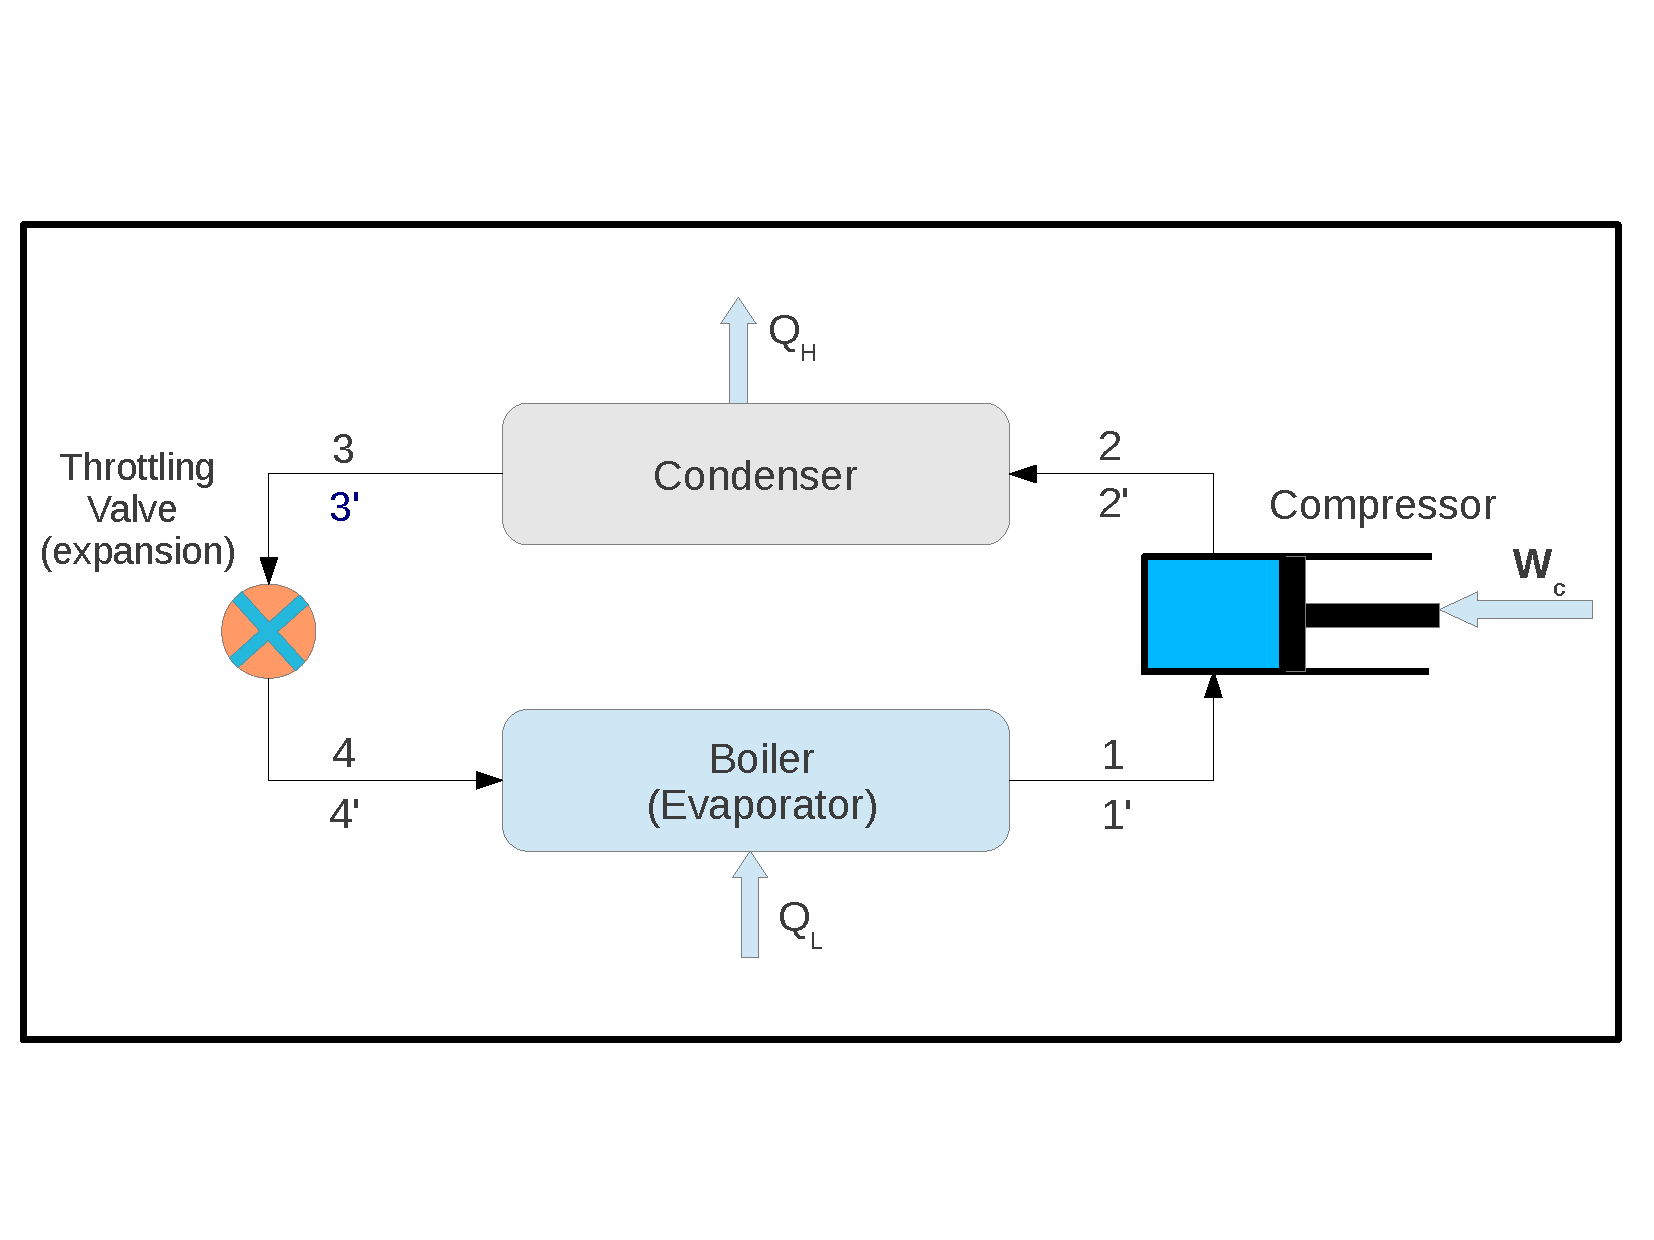
\includegraphics[width=5.8cm,clip]{./Pics/Overview_Refrig12}
     \end{center}
    \end{figure}  
   \end{column}  
   \begin{column}[c]{0.5\linewidth}
  \begin{enumerate}[(a)]
   \item <1-> First vapour-compression refrigeration system was a closed system introduced by Jacob Perkins (1766-1849) using \textcolor{blue}{diethyl ether} as refrigerant fluid;
   \item <2-> Ether vapour was compressed in a piston-cylinder system and condensed (i.e., turned into liquid) at a higher saturation pressure and temperature;
   \item <3-> Liquid ether is throttled through a valve back into the low-pressure evaporator;
   \item <4-> This process takes place beneath the vapour dome of the ether and it is a \textcolor{blue}{reversed Rankine cycle}.
  \end{enumerate}
 \end{column}  
\end{columns}
\end{frame}



%%%
%%% Slide
%%%
\begin{frame}
 \frametitle{Description of the Cycle -- Dry Compression}
  \begin{columns}
   \begin{column}[c]{0.55\linewidth}
    \begin{figure}%
     \vbox{
      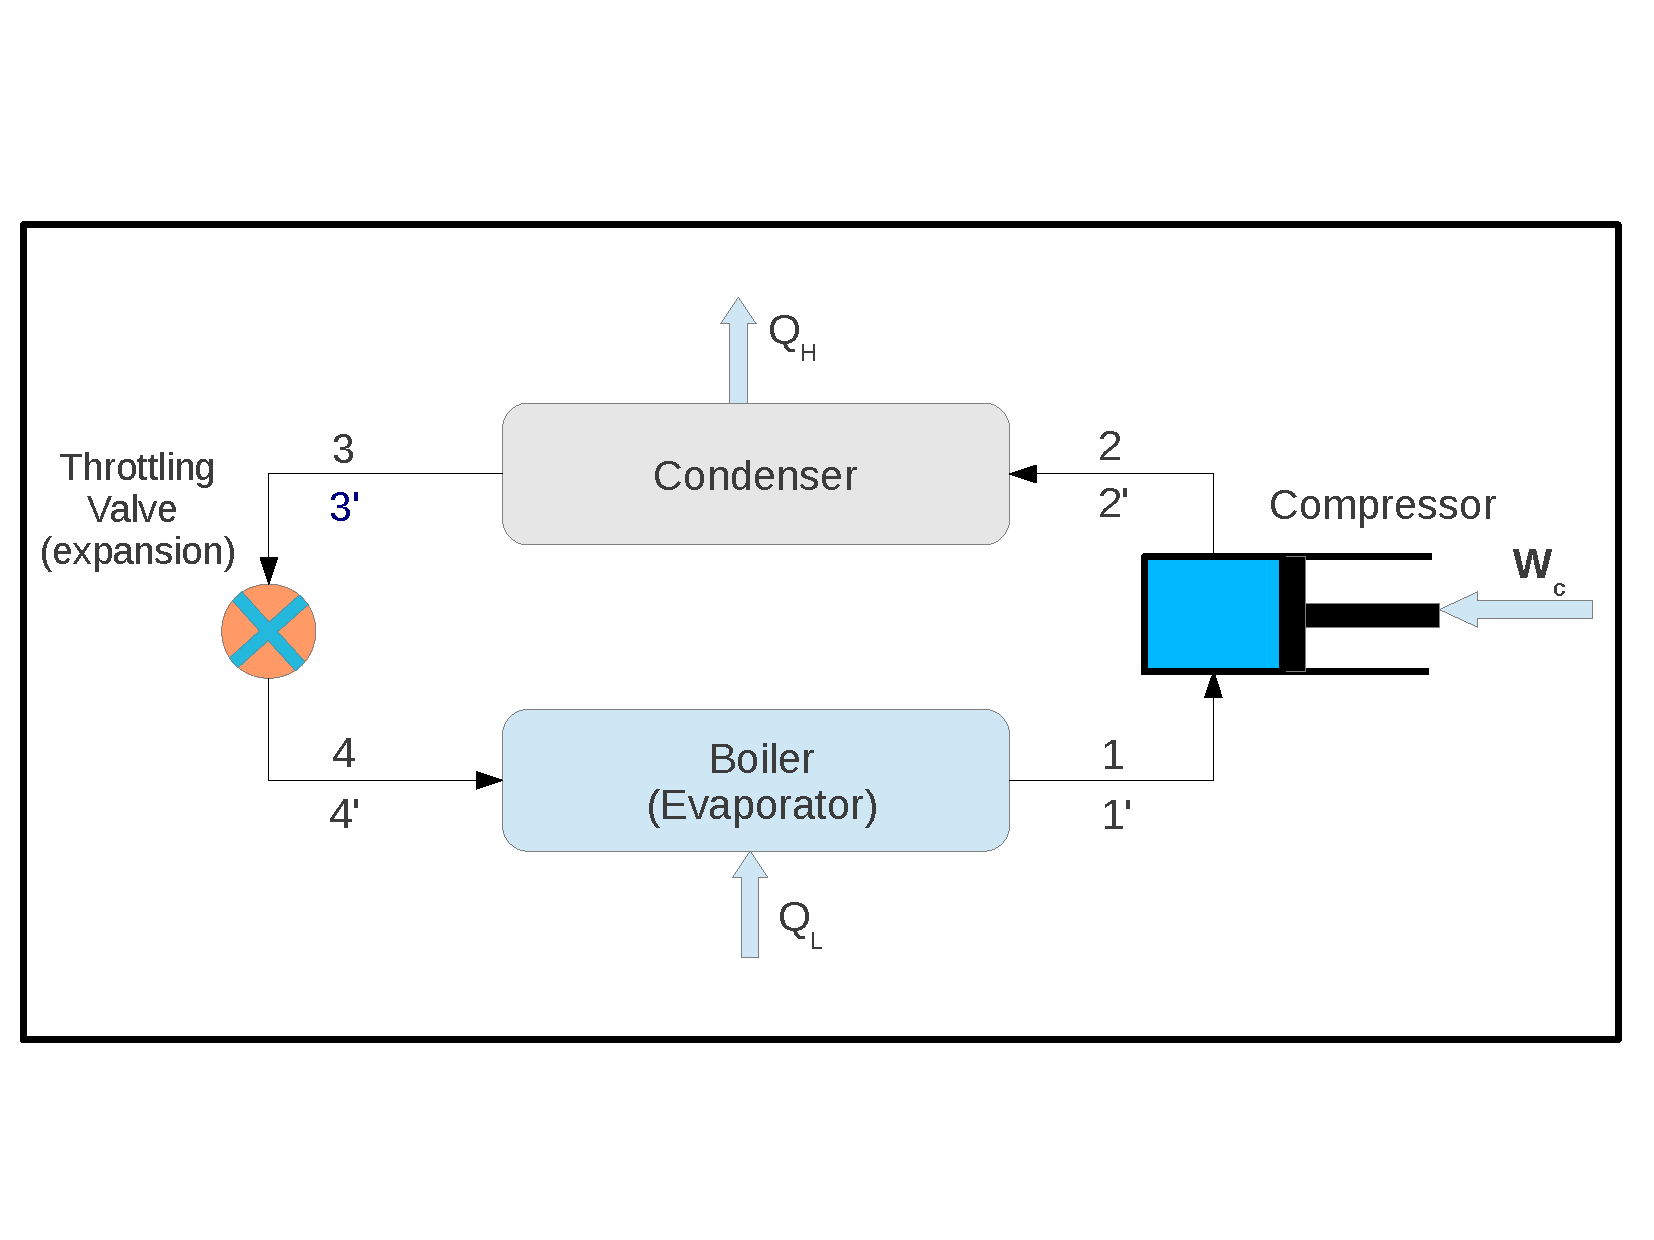
\includegraphics[width=5.5cm,clip]{./Pics/Overview_Refrig12}
      \vspace{-.5cm}
      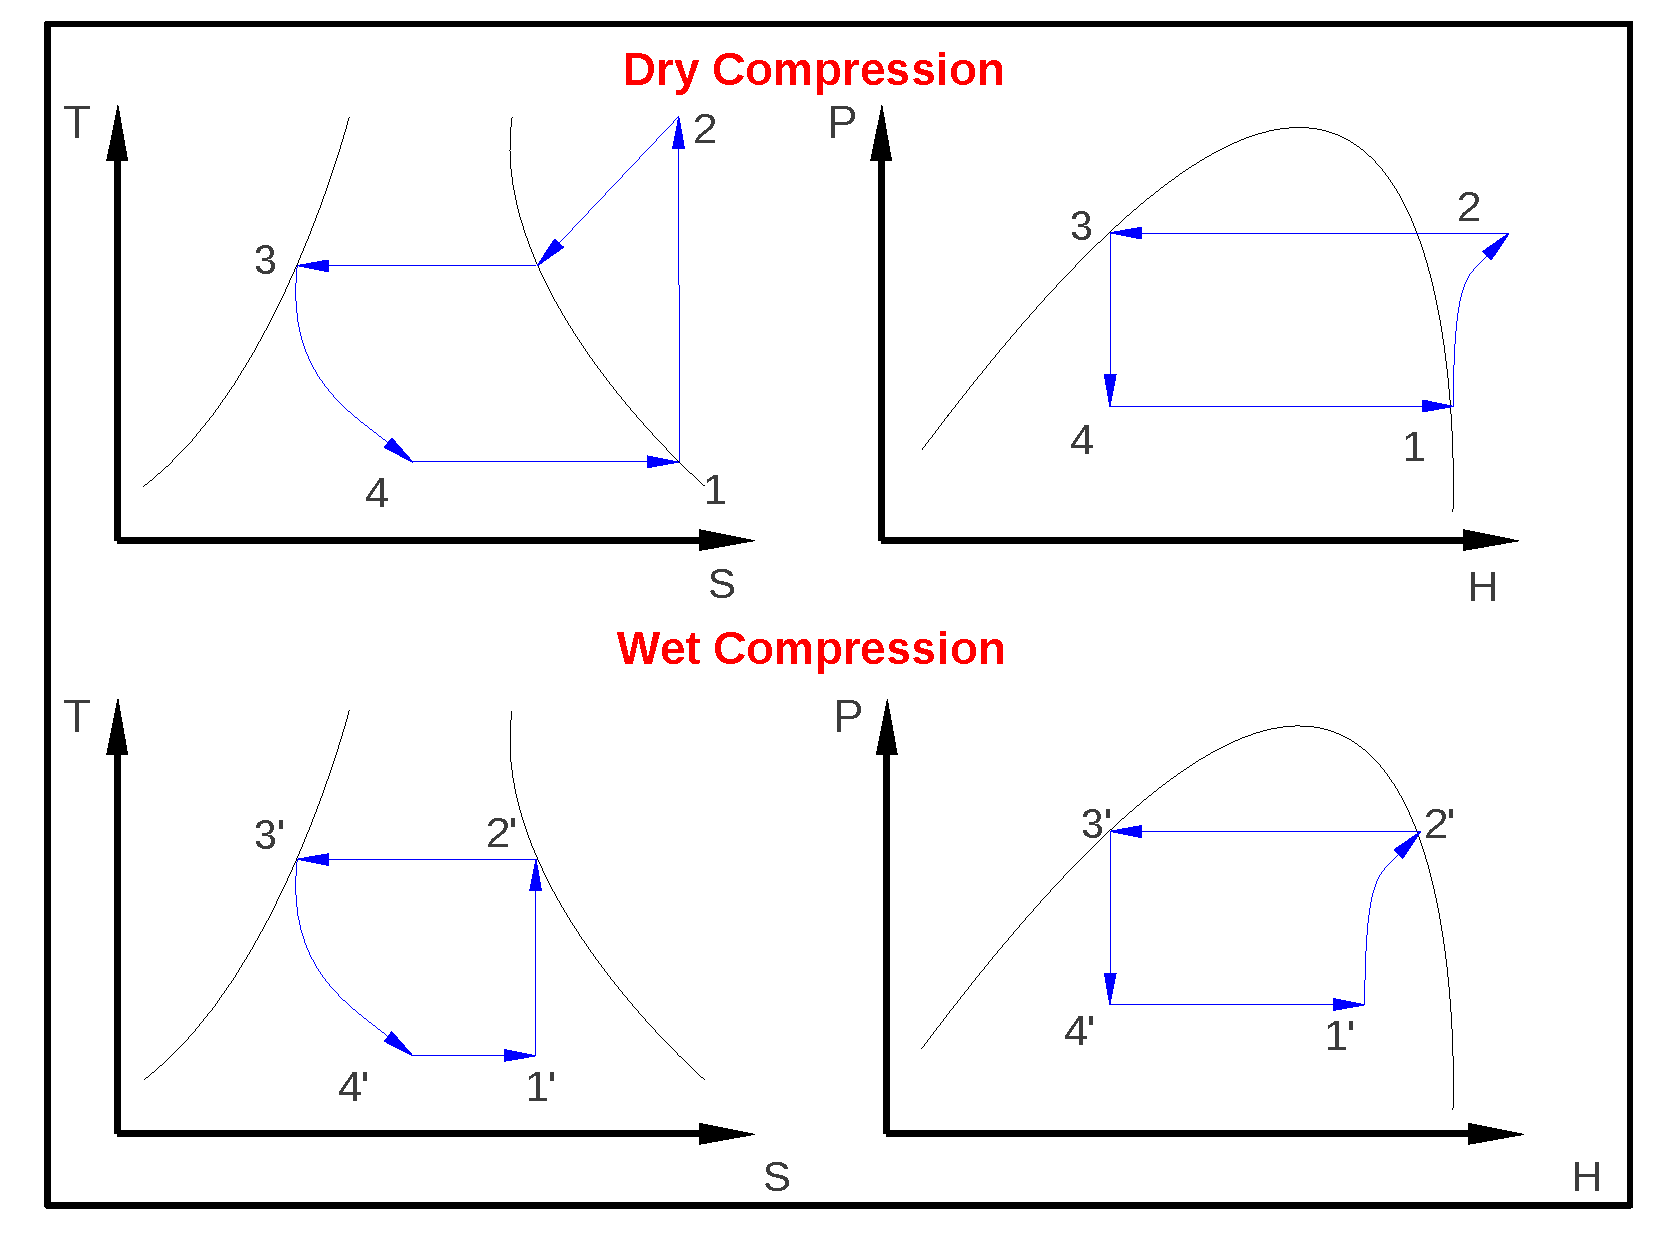
\includegraphics[width=4.5cm,clip]{./Pics/Overview_Refrig13}}
    \end{figure}  
   \end{column}  
   \begin{column}[c]{0.45\linewidth}
  \begin{enumerate}[(a)] 
   \item <1-> In most industrial applications, vapour compression systems occur in closed cycles;
   \item <2-> Refrigerant (in gas/vapour phase) is compressed isentropically in \textcolor{blue}{compressor from state 1 to 2}; 
   \item <3-> \textcolor{blue}{High pressure and high temperature} fluid enters the condenser at \textcolor{blue}{state 2};
   \item <4-> The condensed fluid (saturated liquid at high pressure, state 3) is driven into the expansion valve where an \textcolor{blue}{isenthalpic expansion} occurs.
  \end{enumerate}
 \end{column}  
\end{columns}
\end{frame}


%%%
%%% Slide
%%%
\begin{frame}
 \frametitle{Description of the Cycle -- Dry Compression}
  \begin{columns}
   \begin{column}[c]{0.5\linewidth}
    \begin{figure}%
     \vbox{
      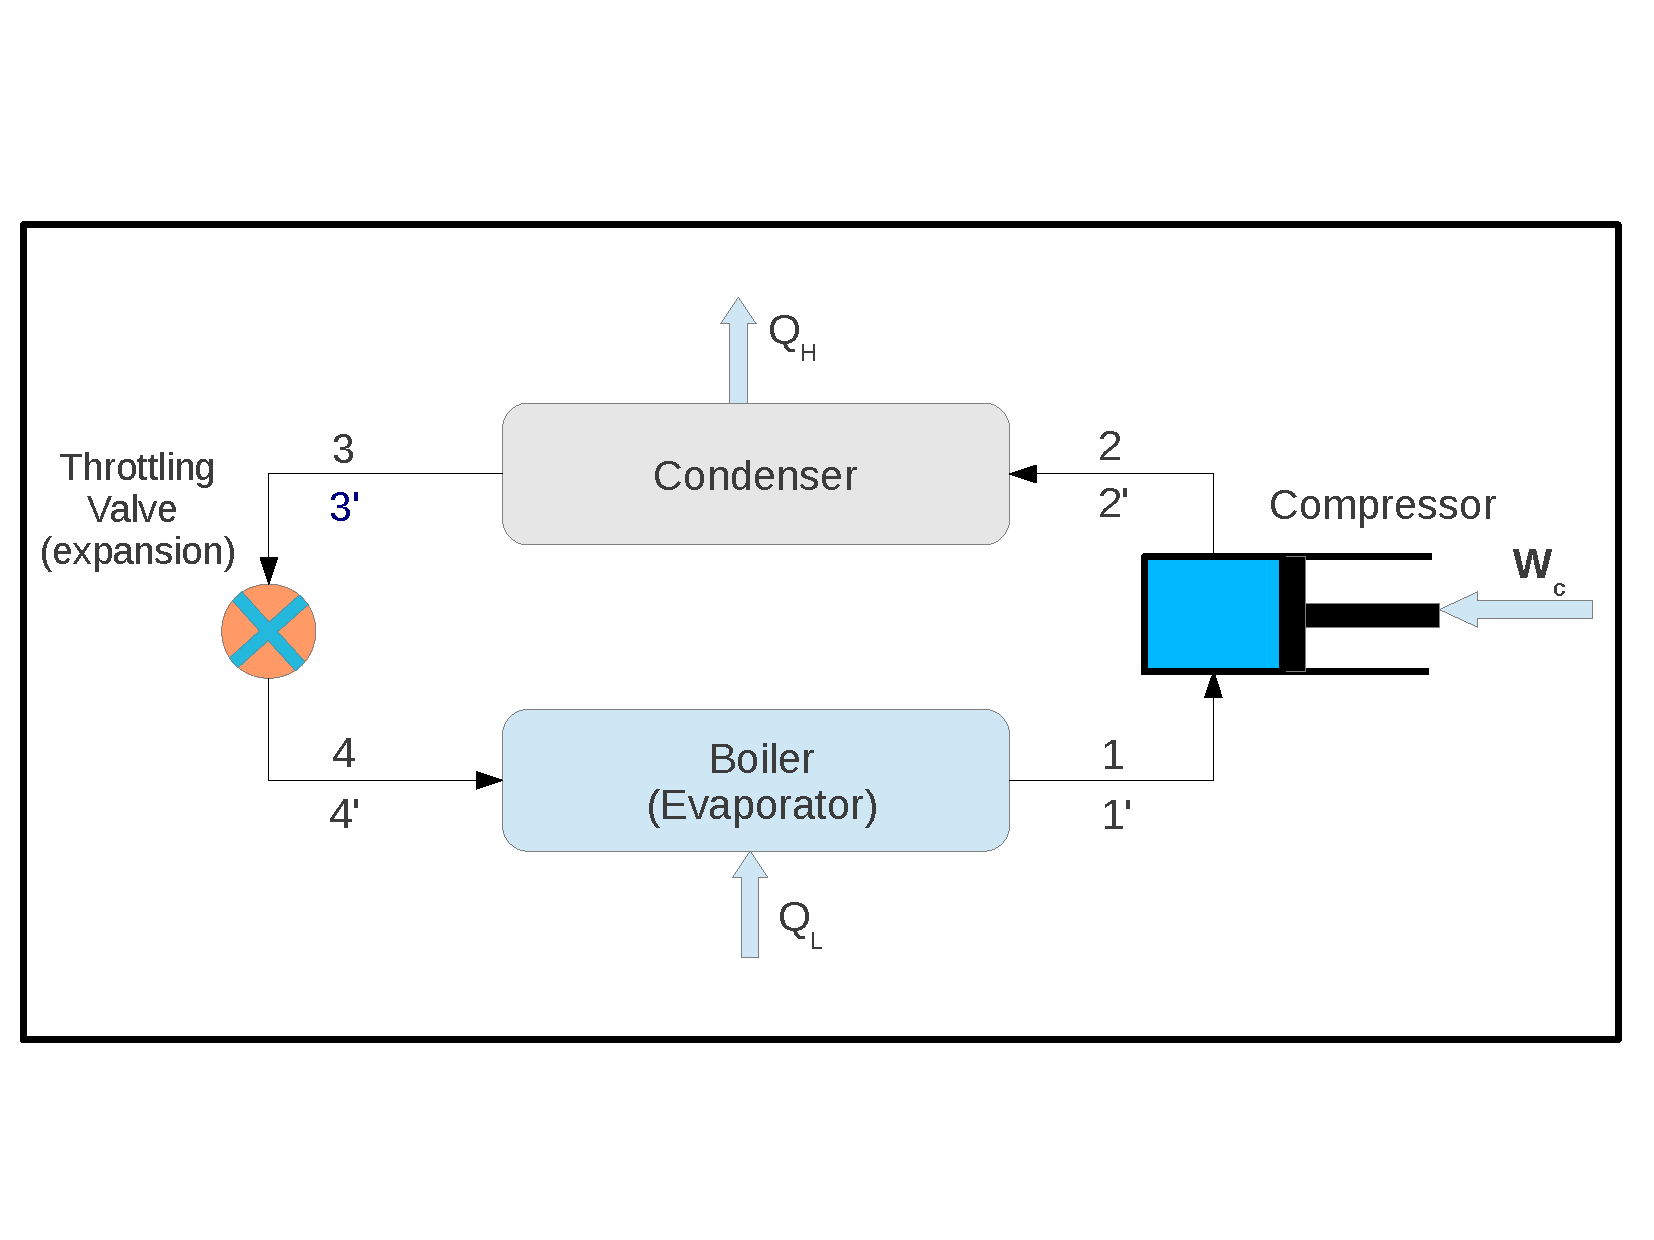
\includegraphics[width=5.5cm,clip]{./Pics/Overview_Refrig12}
      \vspace{-.5cm}
      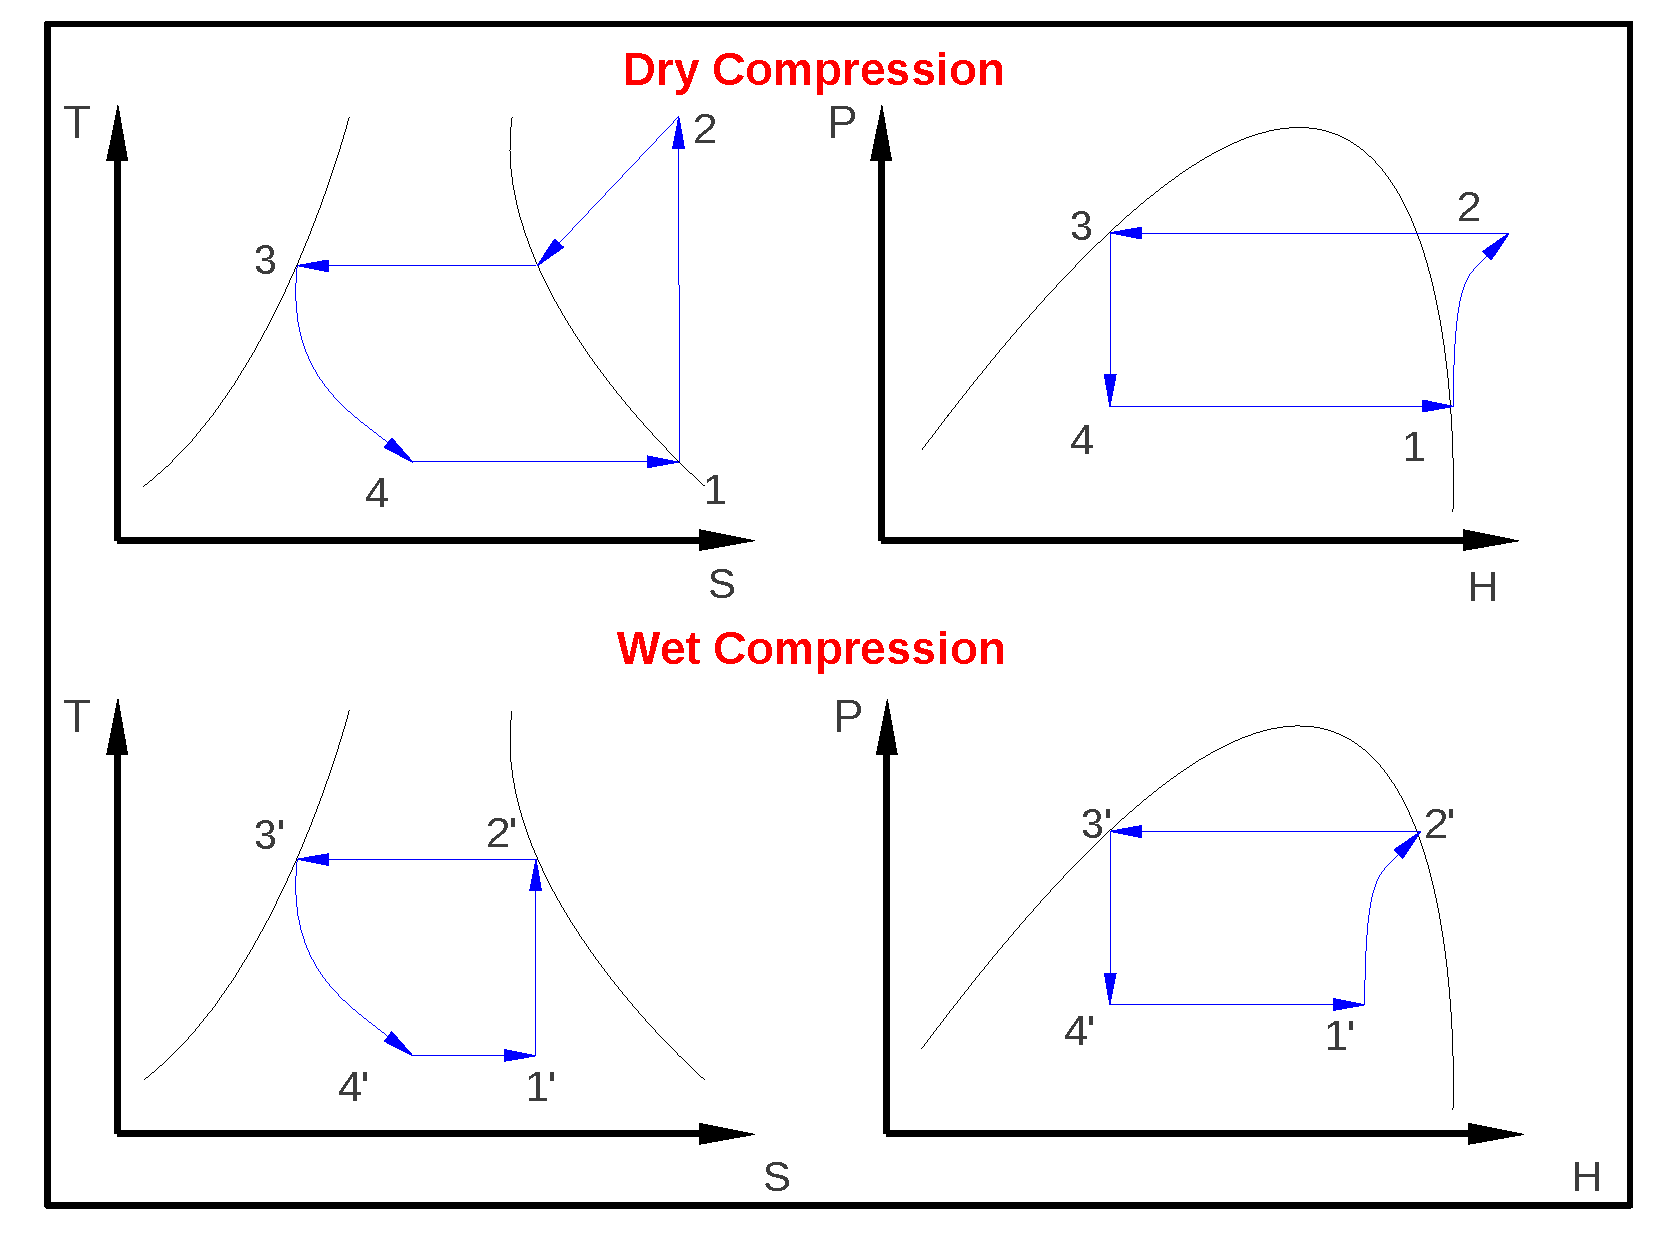
\includegraphics[width=4.5cm,clip]{./Pics/Overview_Refrig13}}
    \end{figure}  
   \end{column}  
   \begin{column}[c]{0.5\linewidth}
  \begin{enumerate}[(a)]\setcounter{enumi}{4}
   \item <1-> The refrigerant fluid leaves the expansion valve (state 4) as a \textcolor{blue}{low pressure wet mixture of liquid and vapour};
   \item <2-> This mixture is driven into the evaporator where heat is transferred from the surroundings and thereby showing refrigerant effect; 
   \item <3-> Due to this \textcolor{blue}{heat absorption}, the liquid-vapour mixture is transformed into a \textcolor{red}{dry gaseous refrigerant} and;
   \item <4-> This process is called \textcolor{blue}{Dry Compression} in which,
   \item <5-> The compression of this dry refrigerant yields \textcolor{blue}{superheated state} of the fluid as shown in \textcolor{blue}{state 2}.
  \end{enumerate}
 \end{column}  
\end{columns}
\end{frame}


%%%
%%% Slide
%%%
\begin{frame}
 \frametitle{Description of the Cycle -- Wet Compression}
  \begin{columns}
   \begin{column}[c]{0.5\linewidth}
    \begin{figure}%
     \vbox{
      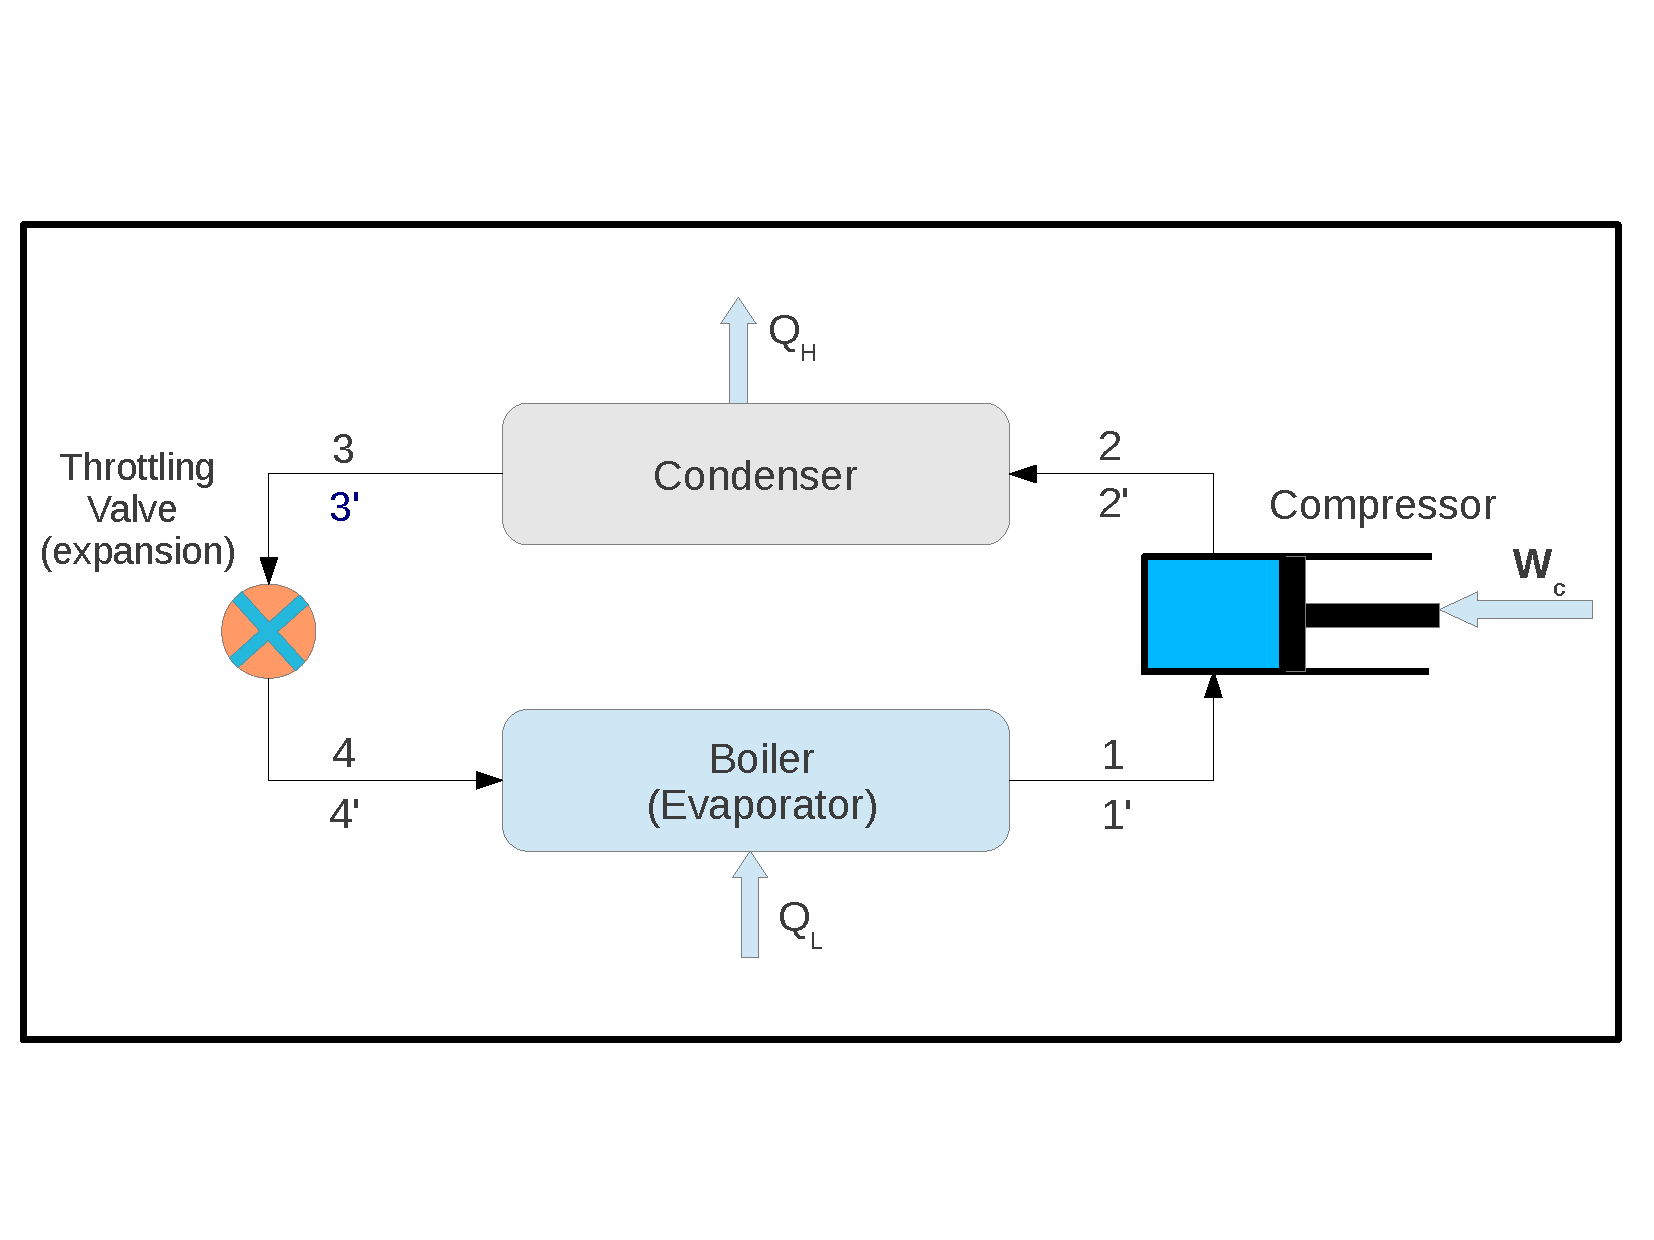
\includegraphics[width=5.5cm,clip]{./Pics/Overview_Refrig12}
      \vspace{-.5cm}
      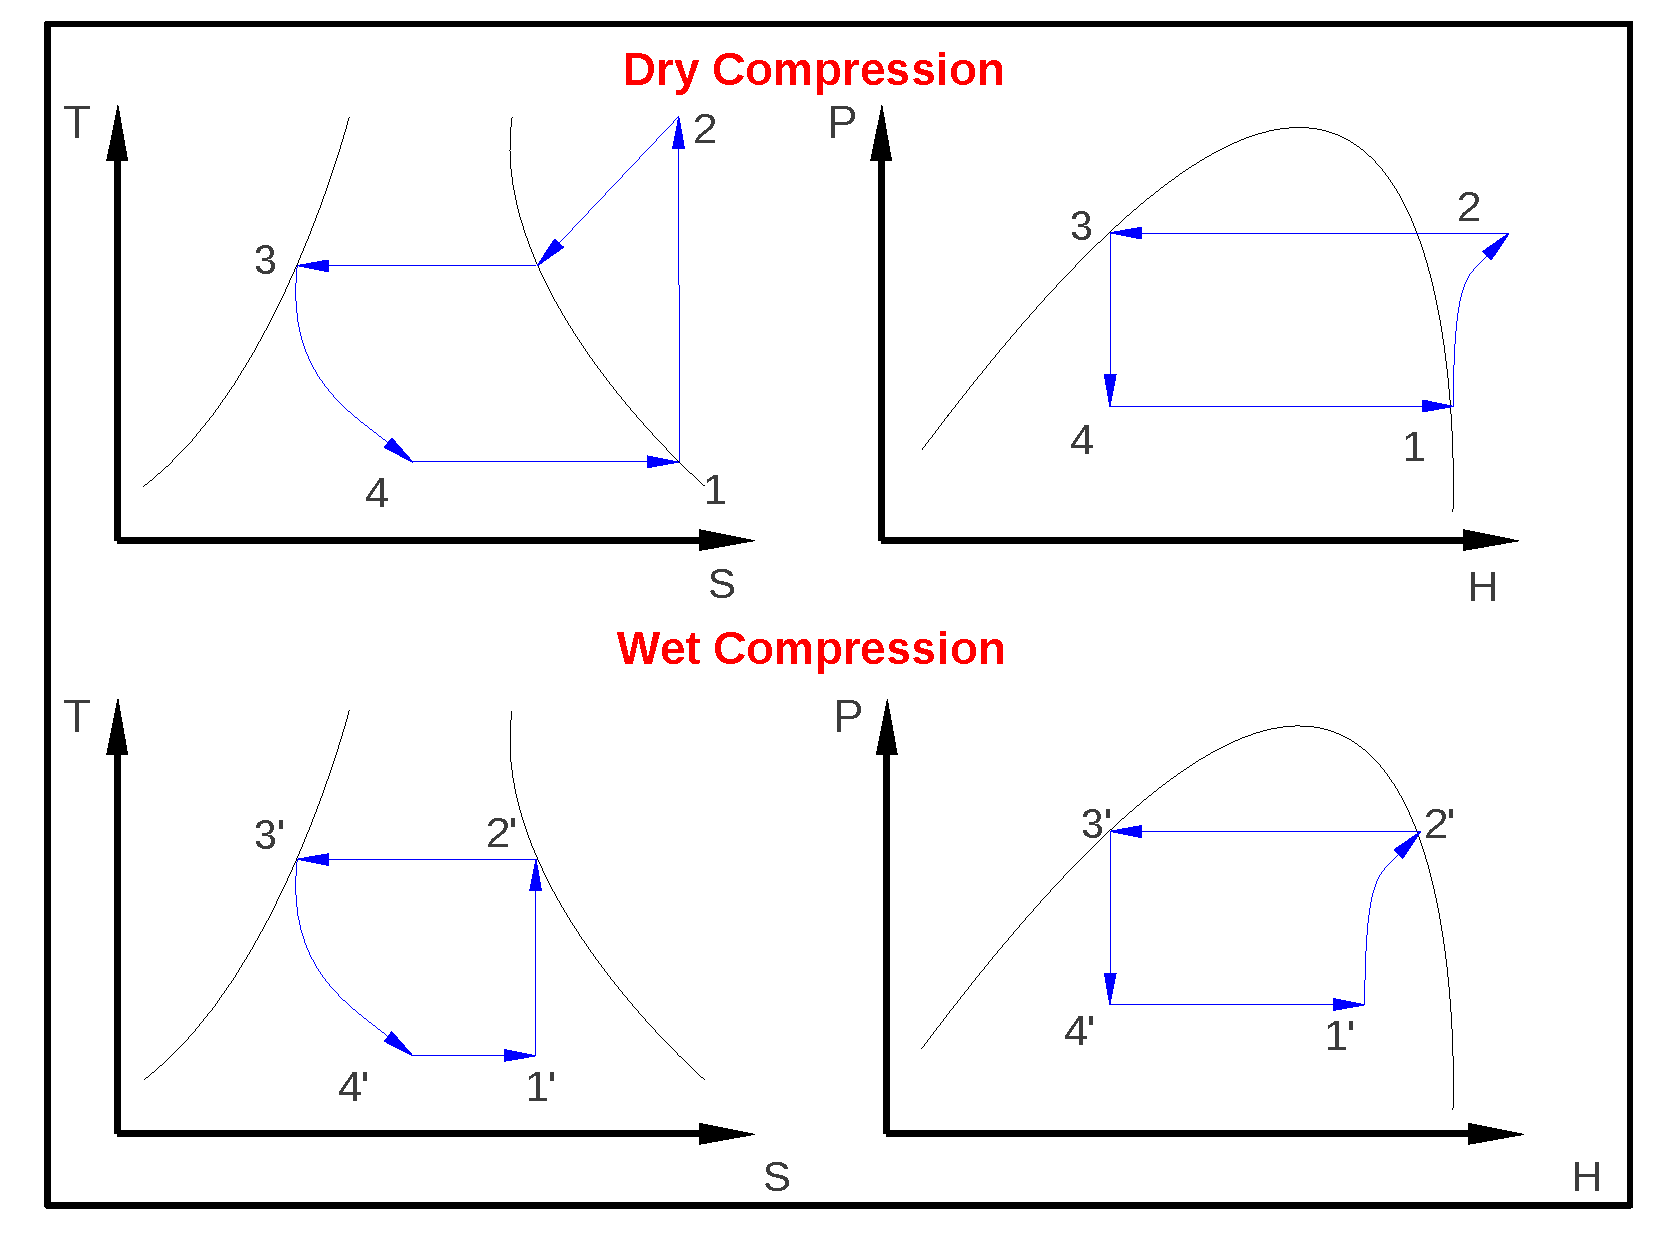
\includegraphics[width=4.5cm,clip]{./Pics/Overview_Refrig13}}
    \end{figure}  
   \end{column}  
   \begin{column}[c]{0.5\linewidth}
  \begin{enumerate}[(a)]
   \item <1-> In this case, the \textcolor{blue}{liquid-vapour mixture (state 1$^{\prime}$)} is injected in the compressor;
   \item <2-> In the compressor, the wet mixture is transformed into a \textcolor{blue}{dry refrigerant fluid} (gas phase -- state 2$^{\prime}$);
   \item <3-> The dry refrigerant at \textcolor{blue}{high pressure and high temperature} is driven into the condenser where the fluid is turned into saturated liquid at high pressure;
  \end{enumerate}
 \end{column}  
\end{columns}
\end{frame}



%%%
%%% Slide
%%%
\begin{frame}
 \frametitle{Description of the Cycle -- Wet Compression}
  \begin{columns}
   \begin{column}[c]{0.5\linewidth}
    \begin{figure}%
     \vbox{
      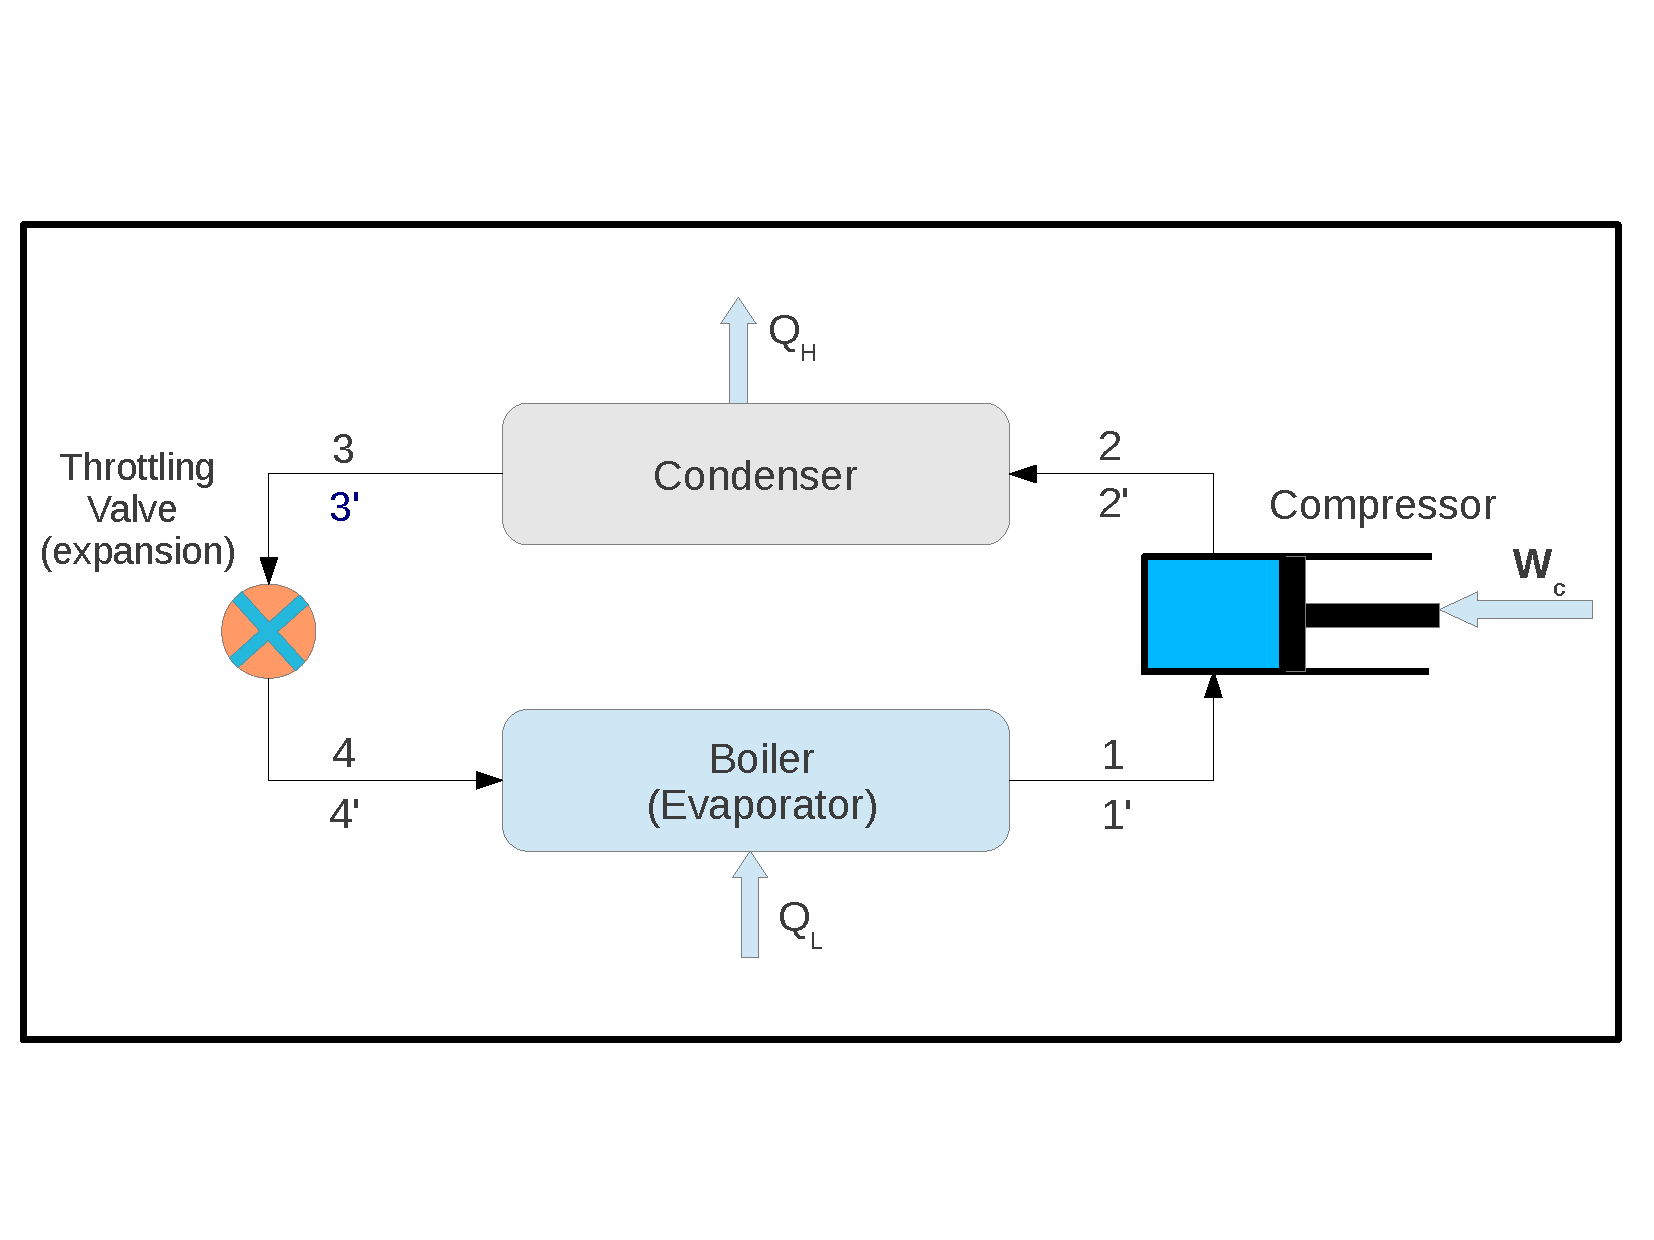
\includegraphics[width=5.5cm,clip]{./Pics/Overview_Refrig12}
      \vspace{-.5cm}
      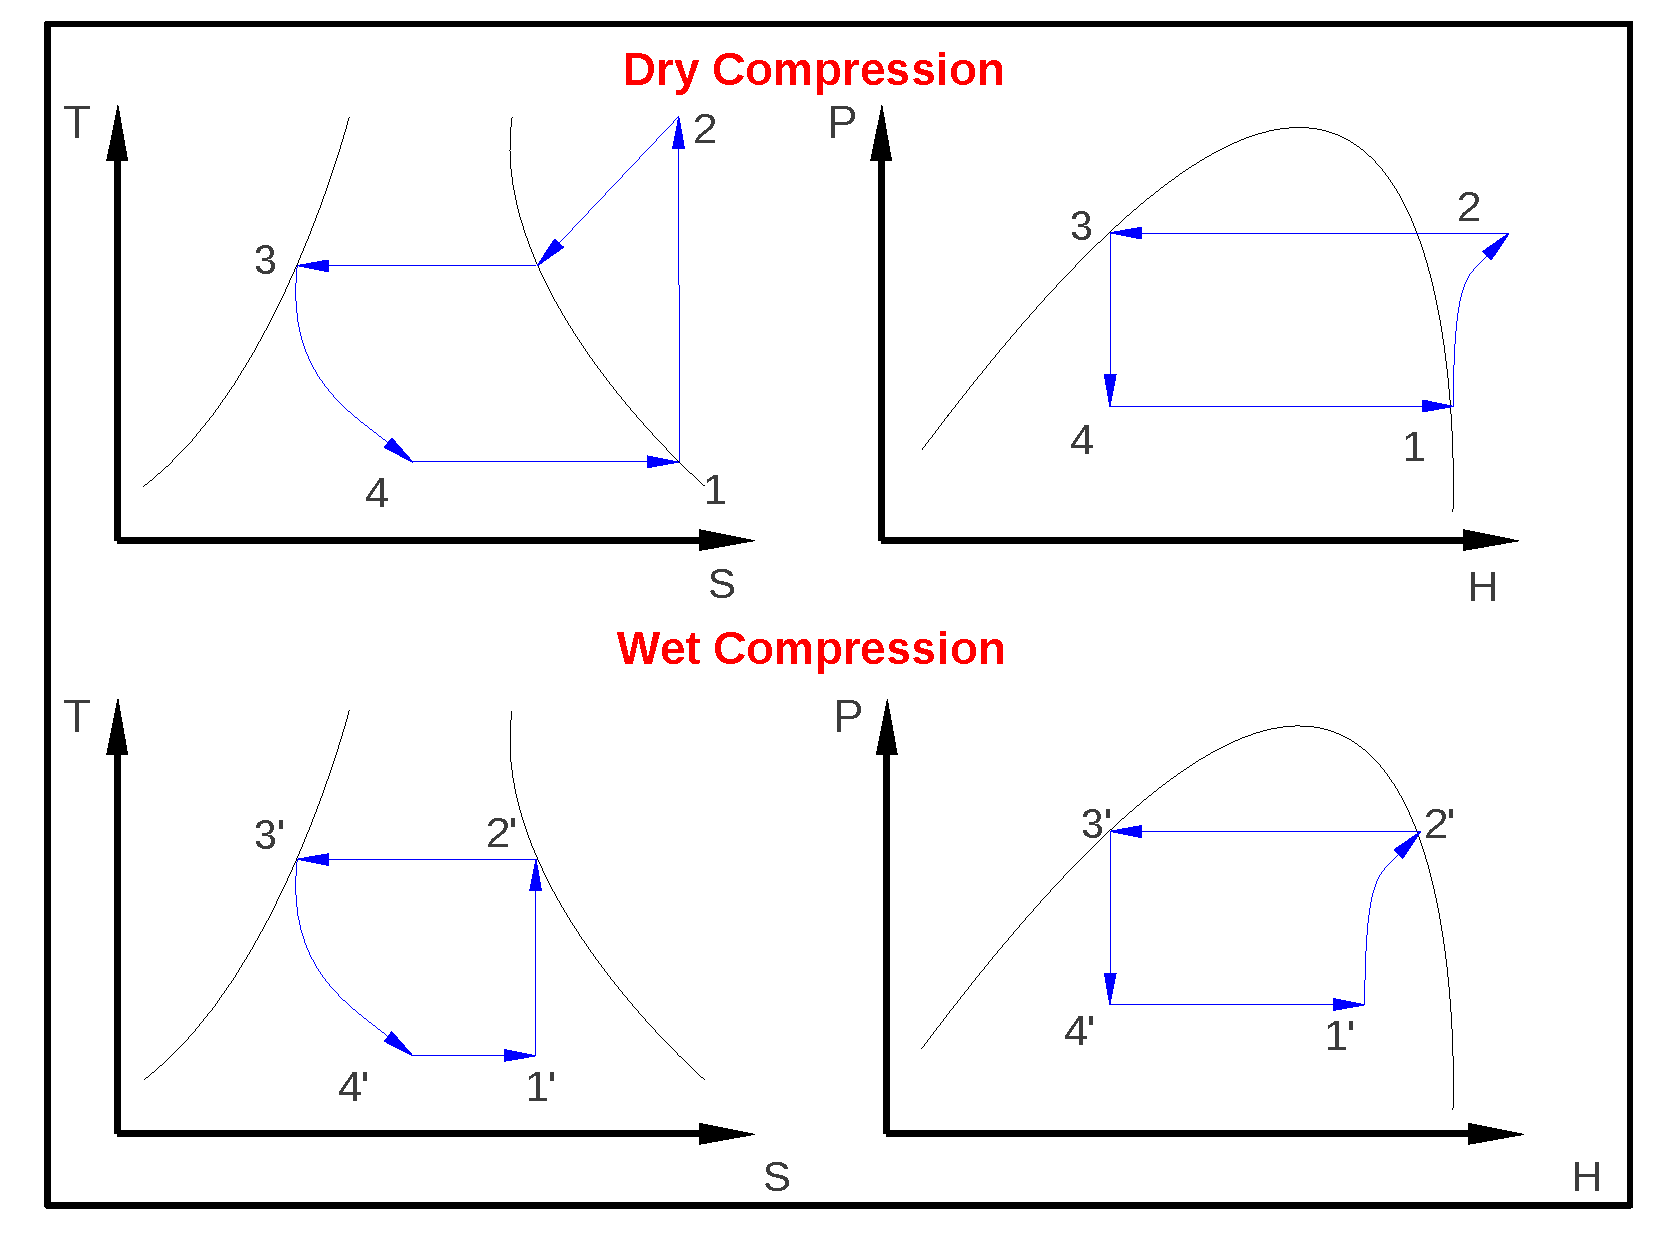
\includegraphics[width=4.5cm,clip]{./Pics/Overview_Refrig13}}
    \end{figure}  
   \end{column}  
   \begin{column}[c]{0.5\linewidth}
  \begin{enumerate}[(a)]\setcounter{enumi}{3}
   \item <1-> The refrigerant is throttled from high to low pressure inside the expansion valve (states 3$^{\prime}$-4$^{\prime}$);
   \item <2-> The refrigerant is then driven towards the evaporator (states 4$^{\prime}$ 1$^{\prime}$) where it absorbs heat from the surroundings and ;
   \item <3-> Part of the liquid fraction is evaporated \textcolor{red}{but it does not become dry (gas) refrigerant} at the inlet of the compressor.
  \end{enumerate}
 \end{column}  
\end{columns}
\end{frame}



%%%
%%% Slide
%%%
\begin{frame}
 \frametitle{Description of the Cycle -- In Summary:}
  \begin{columns}
   \begin{column}[c]{0.5\linewidth}
    \begin{figure}%
     \vbox{
      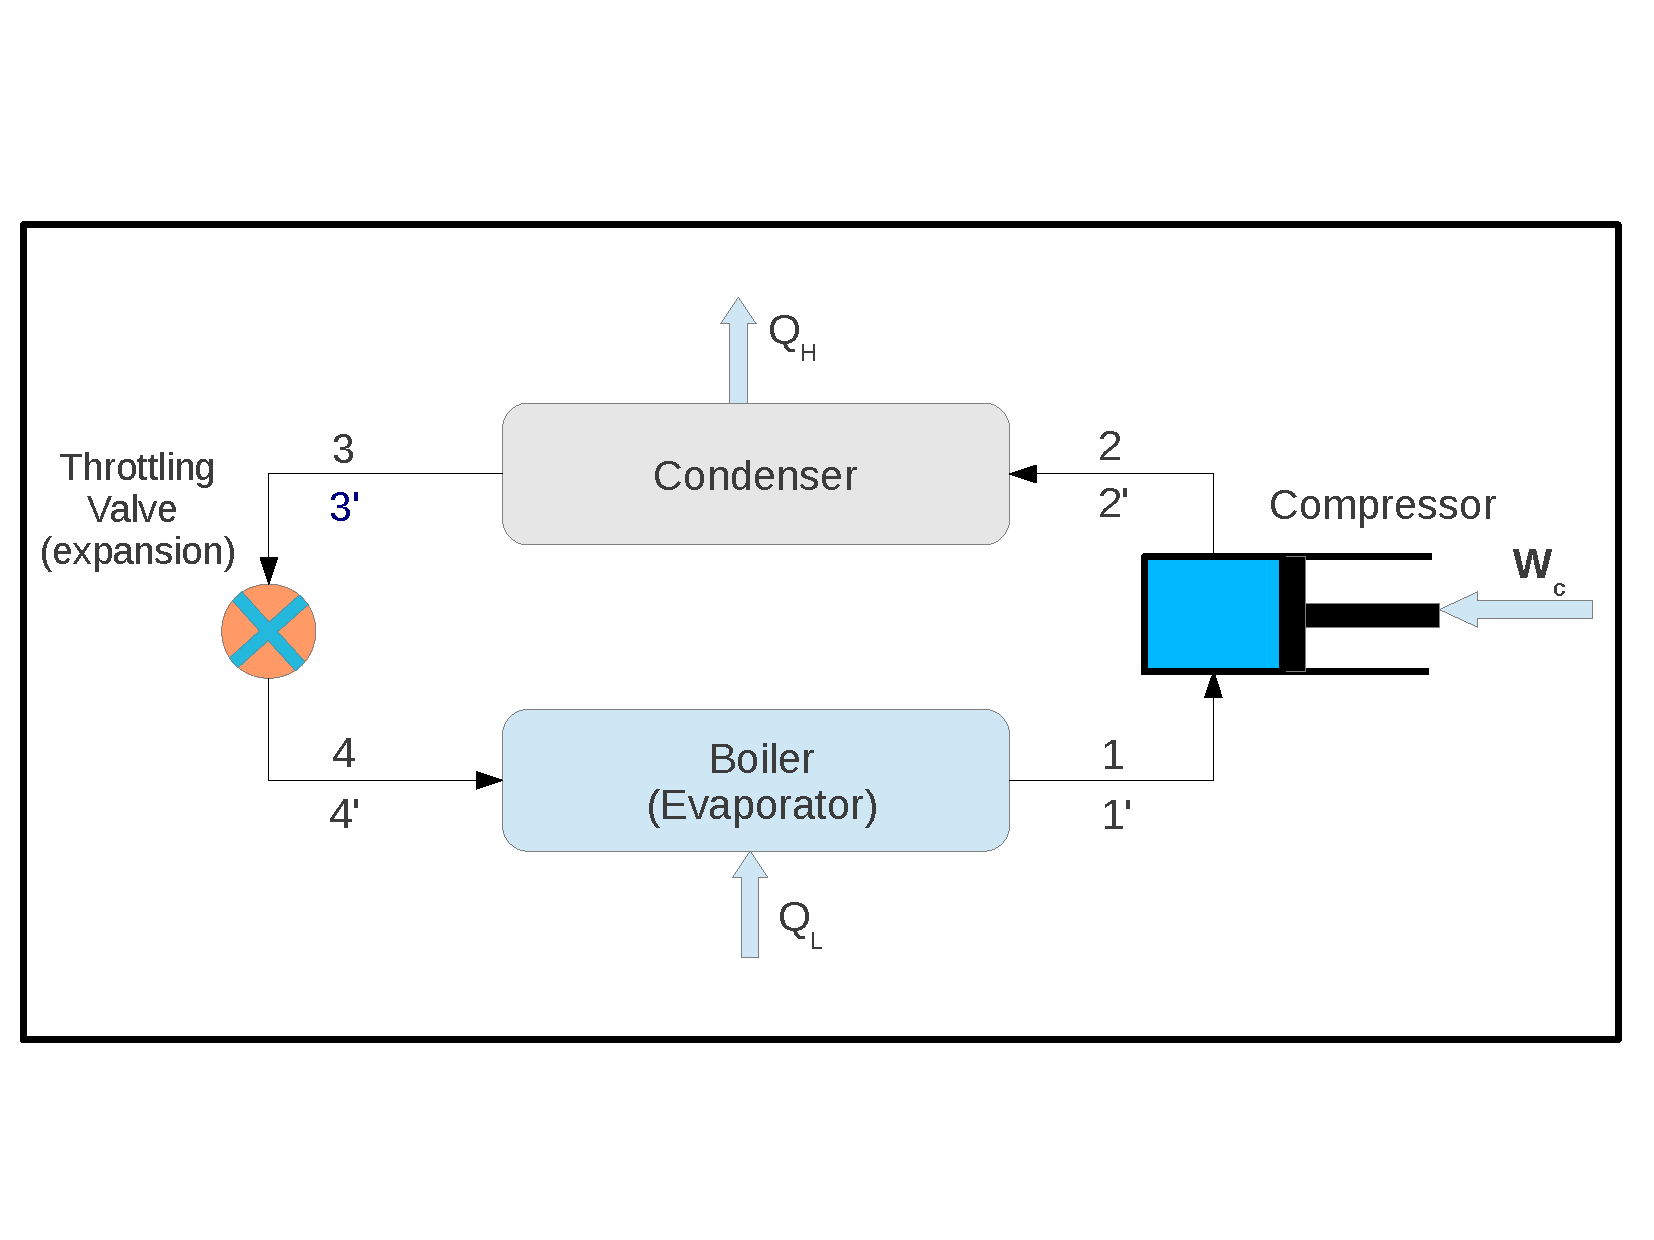
\includegraphics[width=5.5cm,clip]{./Pics/Overview_Refrig12}
      \vspace{-.5cm}
      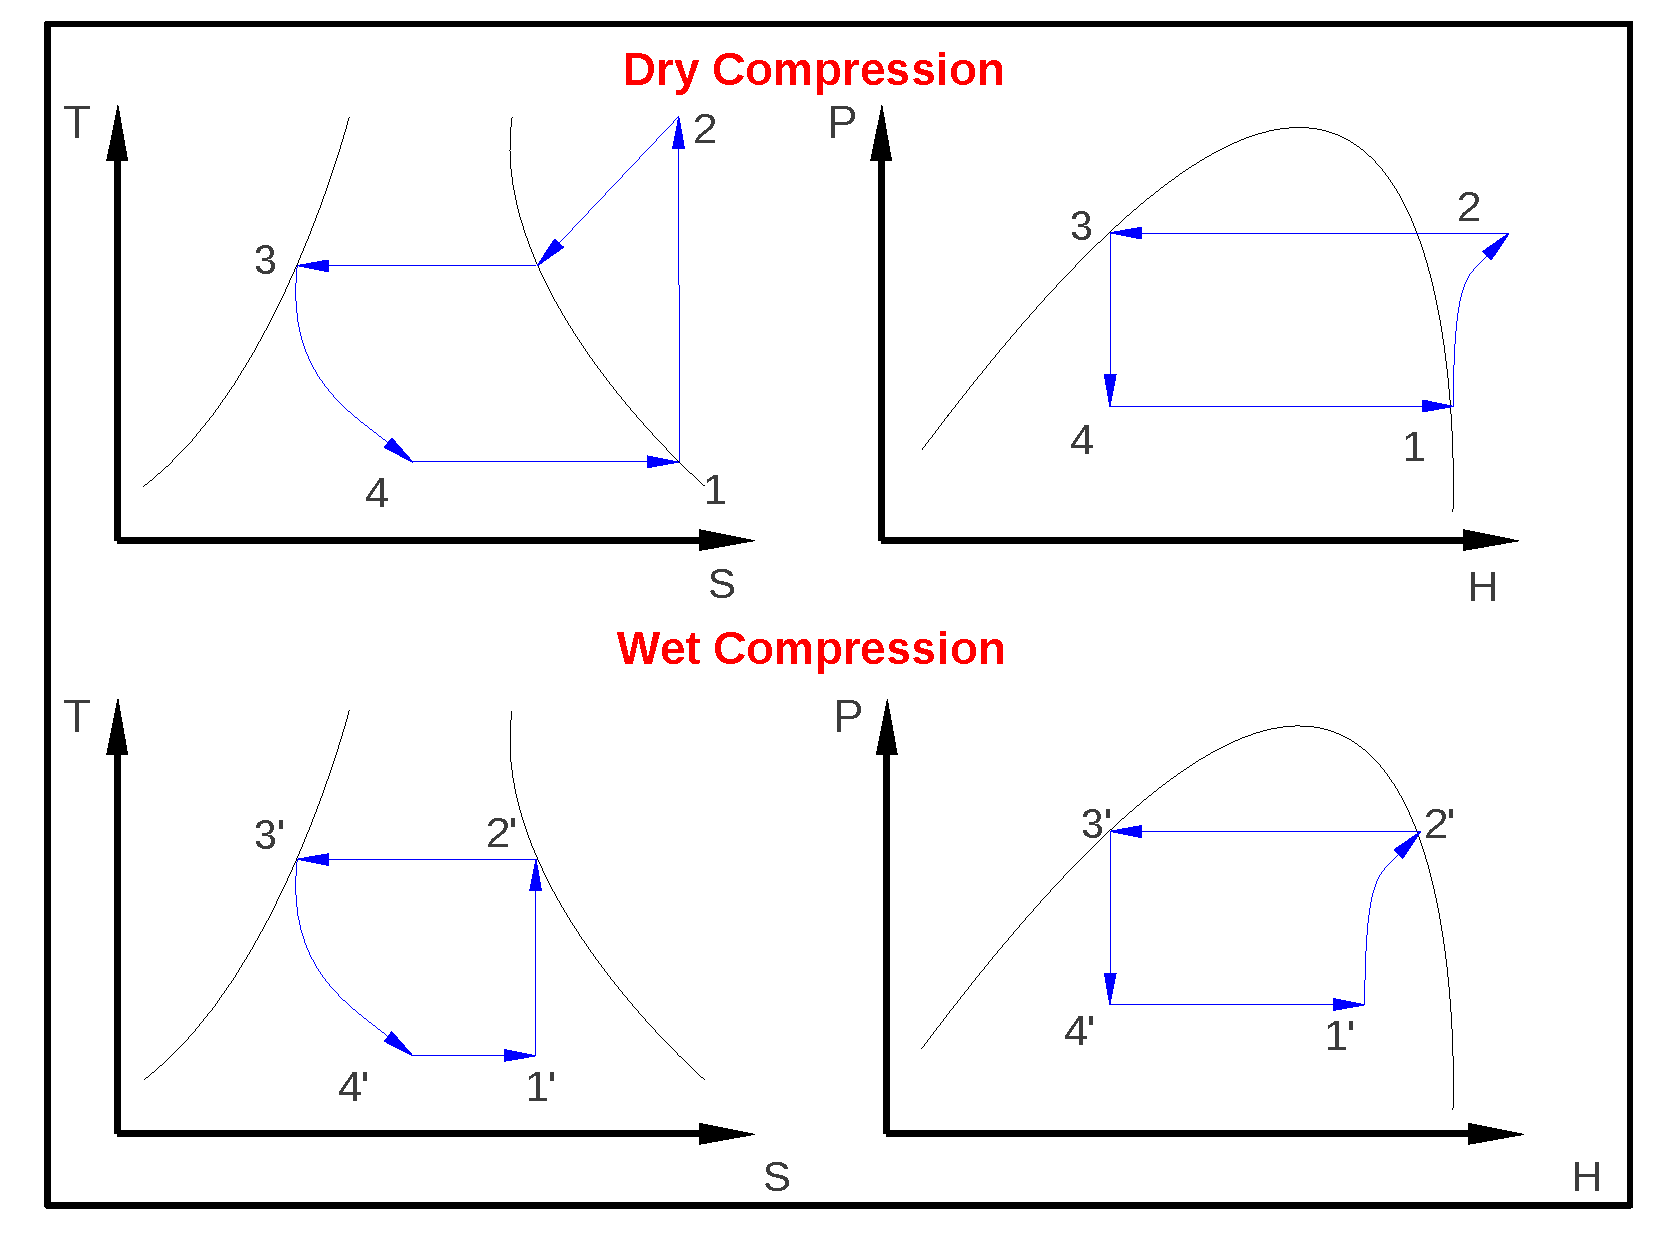
\includegraphics[width=4.5cm,clip]{./Pics/Overview_Refrig13}}
    \end{figure}  
   \end{column}  
   \begin{column}[c]{0.5\linewidth}
  \begin{itemize}
   \item <1-> \textcolor{blue}{1-2} or \textcolor{blue}{1$^{\prime}$-2$^{\prime}$:} isentropic compression;
   \item <1-> \textcolor{blue}{2-3} or \textcolor{blue}{2$^{\prime}$-3$^{\prime}$:} isobaric heat rejection;
   \item <1-> \textcolor{blue}{3-4} or \textcolor{blue}{3$^{\prime}$-4$^{\prime}$:} isenthalpic expansion ;%process or throttling process;
   \item <1-> \textcolor{blue}{4-1} or \textcolor{blue}{4$^{\prime}$-1$^{\prime}$:} isobaric heat absorption.
  \end{itemize}
 \end{column}  
\end{columns}
\end{frame}


%%%
%%% SUBSECTION
%%
\subsection{Thermal Analysis}
%%%
%%% Slide
%%%
\begin{frame}
 \frametitle{Thermal Analysis -- 3 Scenarios/Strategies}
 \begin{columns}
  \begin{column}[c]{0.65\linewidth}
   \begin{figure}%
     \vbox{
      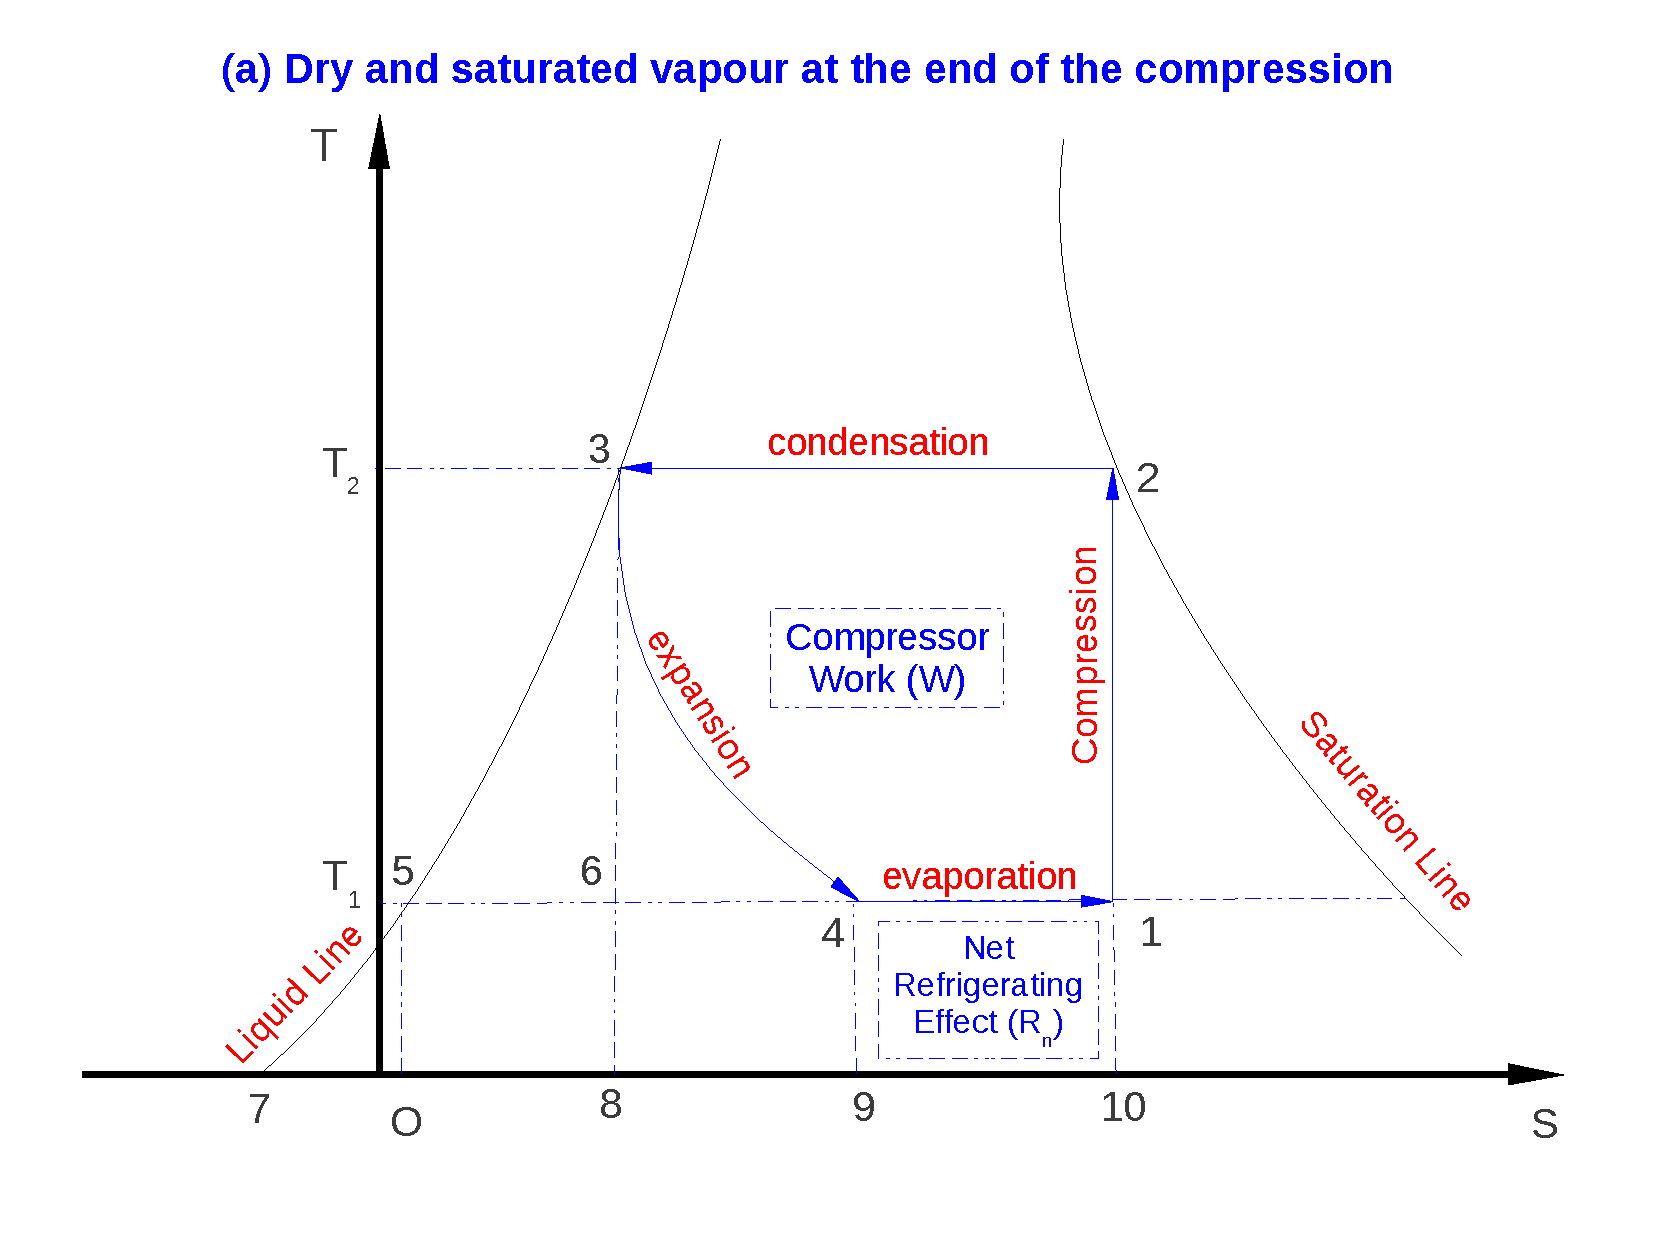
\includegraphics[width=5.4cm,height=2.6cm,clip]{./Pics/Overview_Refrig14}
      \vspace{-.1cm}
      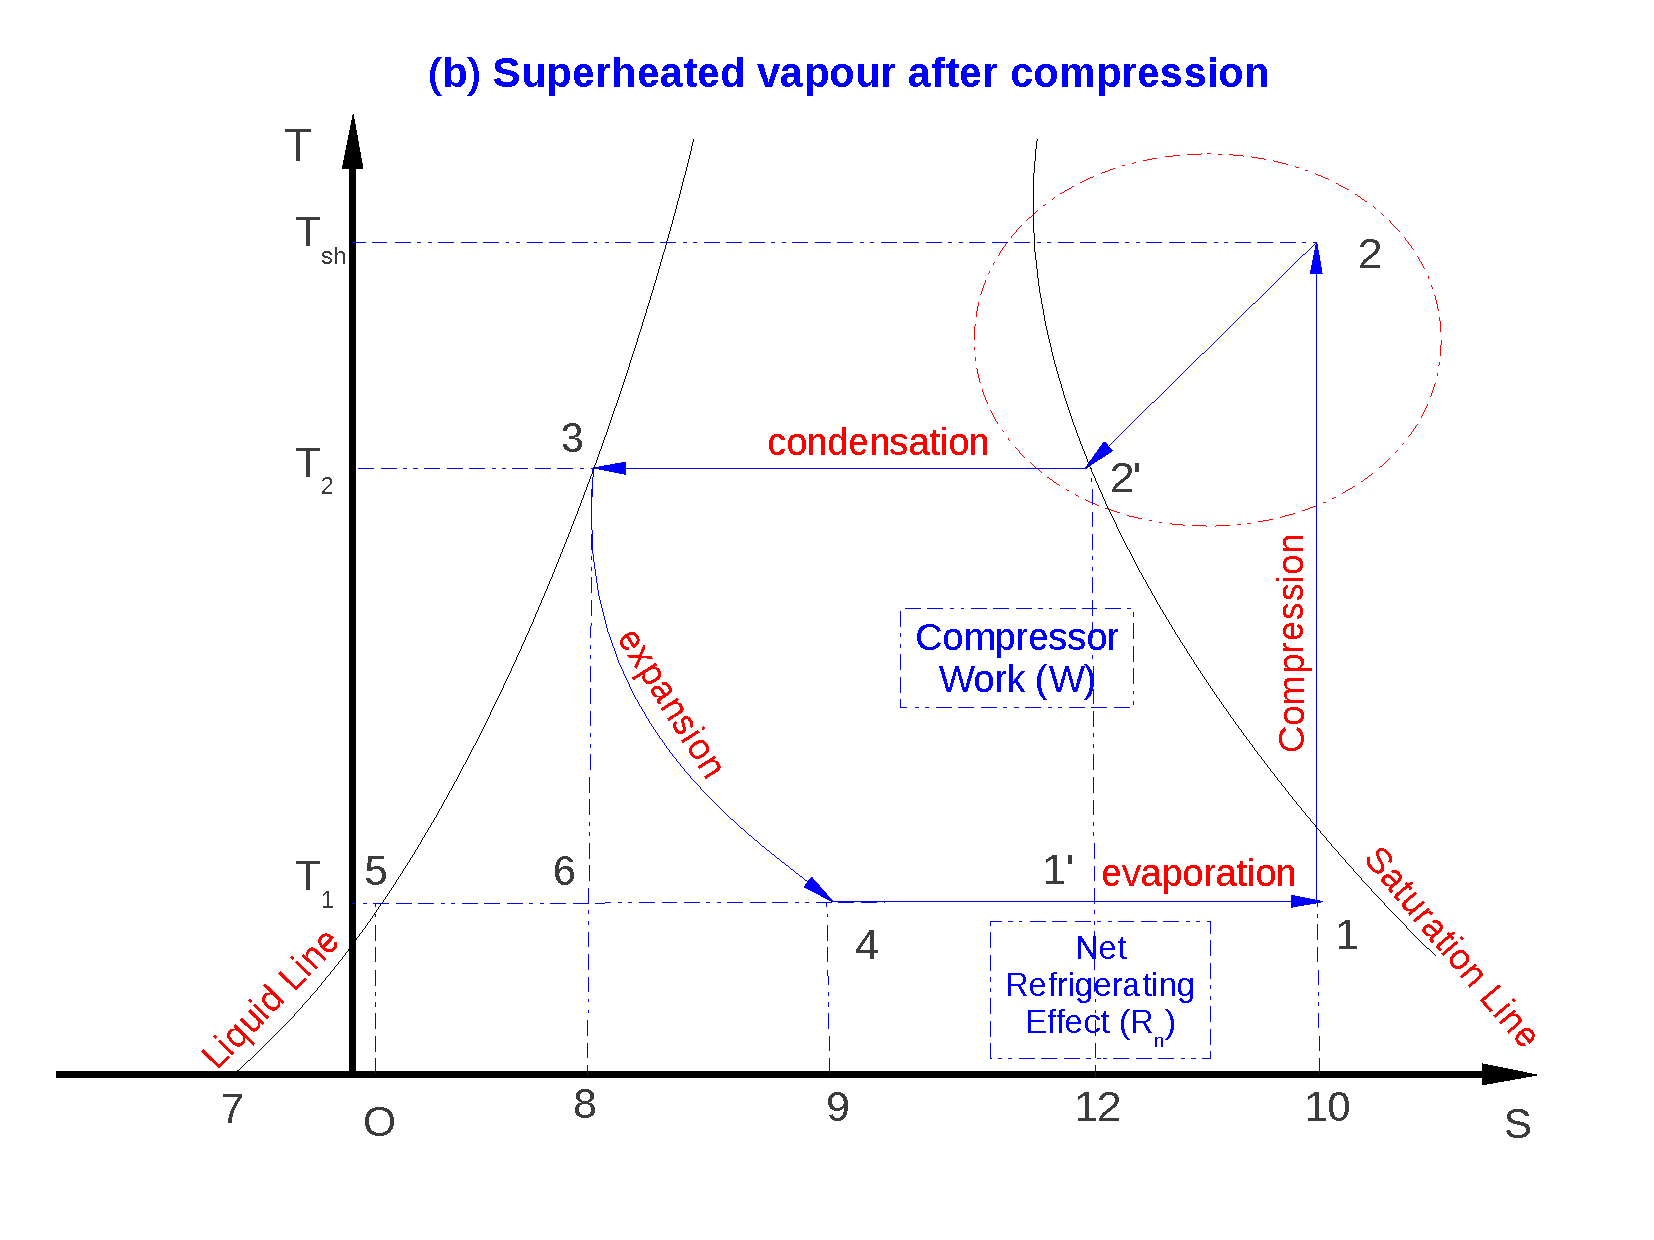
\includegraphics[width=5.4cm,height=2.6cm,clip]{./Pics/Overview_Refrig15}
      \vspace{-.1cm}
      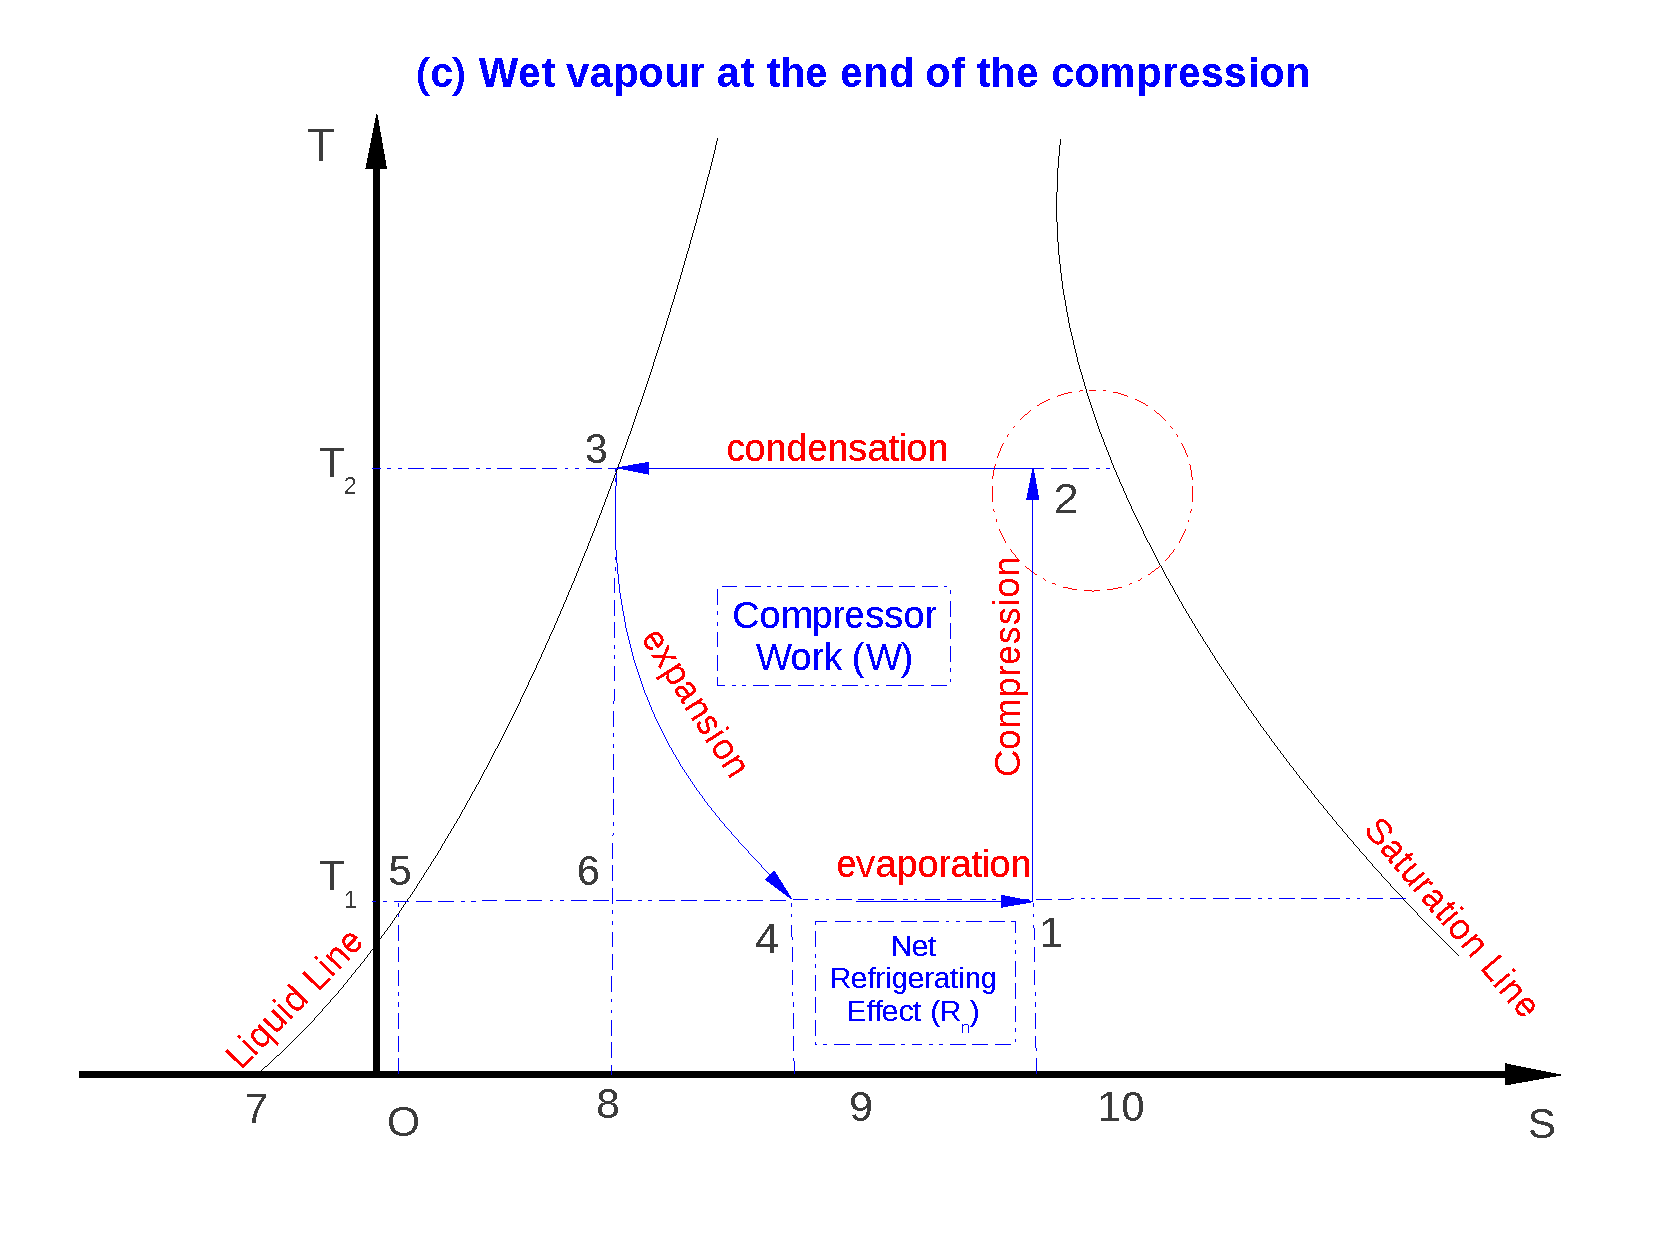
\includegraphics[width=5.4cm,height=2.6cm,clip]{./Pics/Overview_Refrig16}}
   \end{figure}  
  \end{column}  
  \begin{column}[c]{0.35\linewidth}
The \textcolor{blue}{Temperature-Entropy diagram} of the vapour-compression cycle leads to 3 important cases:
   \begin{enumerate}[(a)]
    \item <2-> Vapour is dry and saturated at the end of the compression;
    \item <3-> Vapour is superheated after compression and;
    \item <4-> Vapour is wet after compression.
   \end{enumerate}
  \end{column}  
 \end{columns}
\end{frame}




%%%
%%% Slide
%%%
\begin{frame}
 \frametitle{Thermal Analysis}
 \begin{columns}
  \begin{column}[c]{0.55\linewidth}
   \begin{figure}%
     \vbox{
      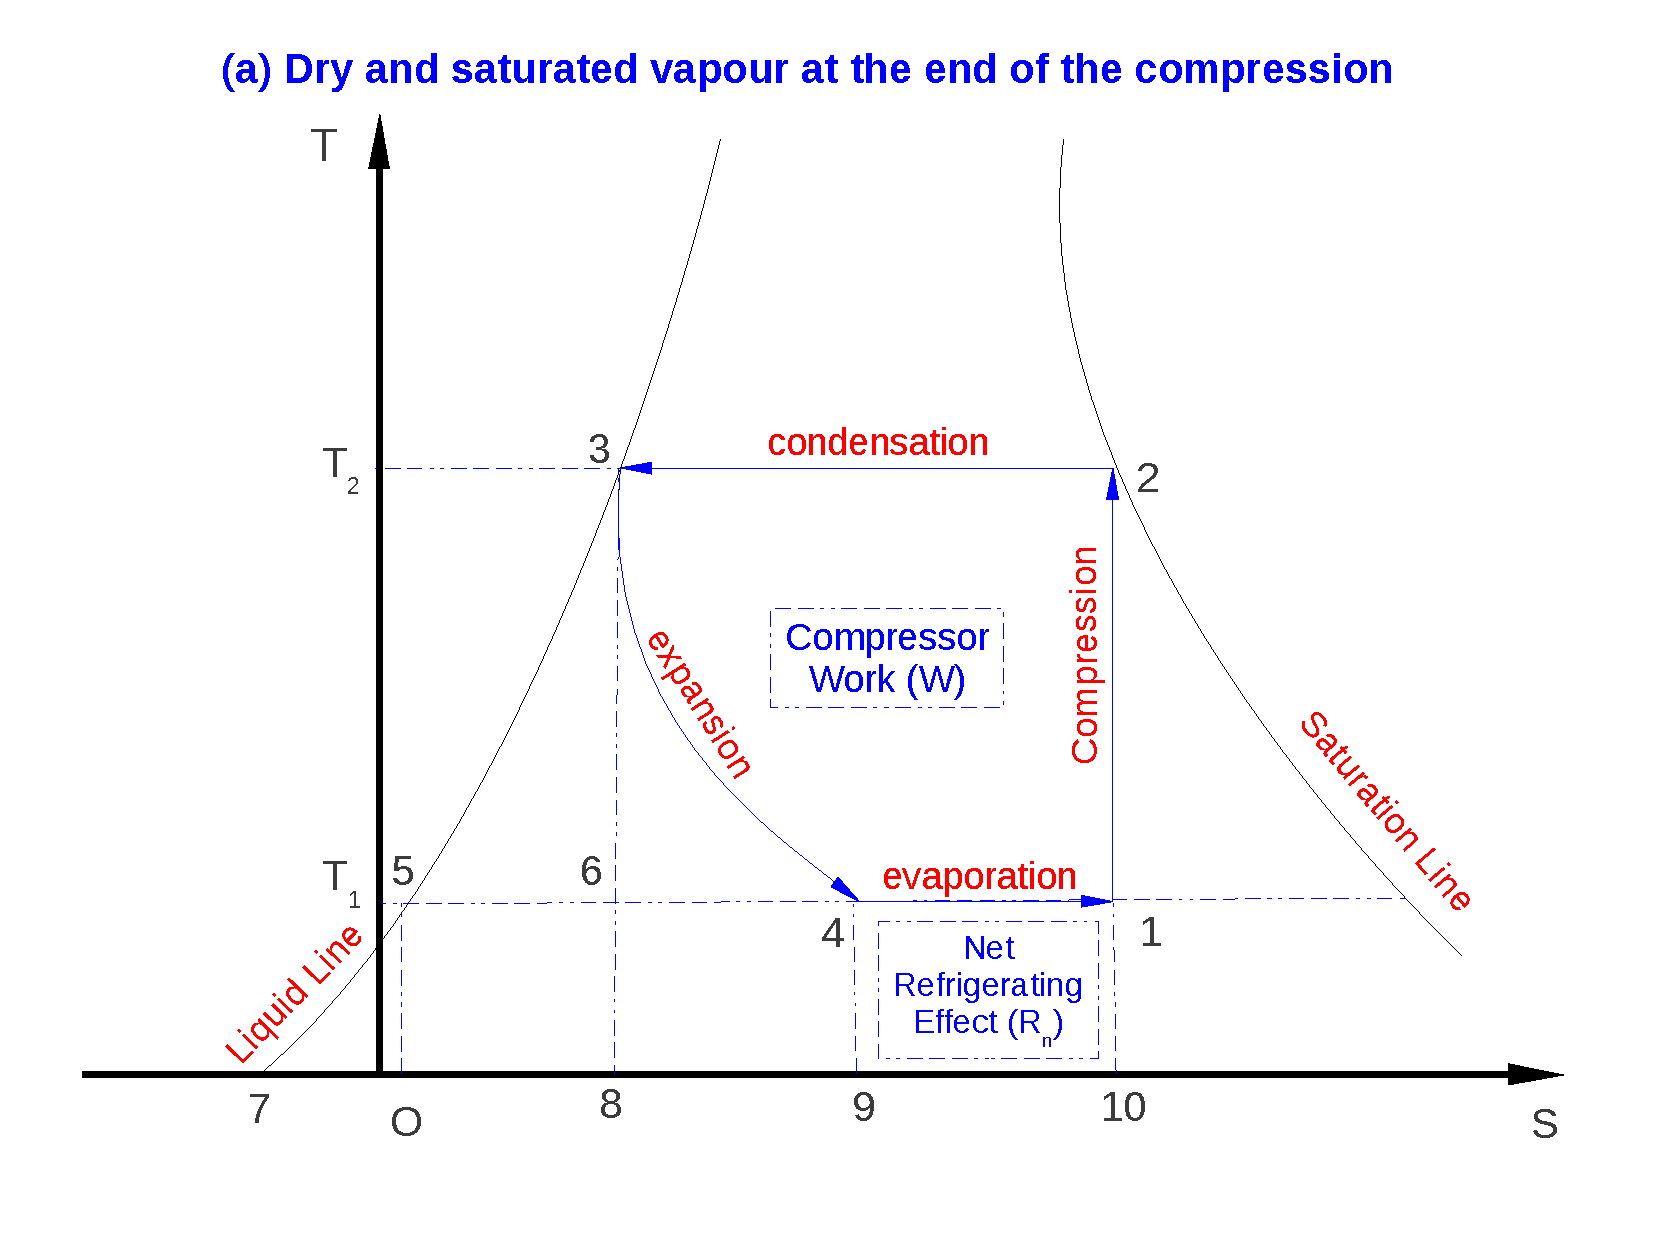
\includegraphics[width=4.cm,height=2.4cm,clip]{./Pics/Overview_Refrig14}
      \vspace{-.1cm}
      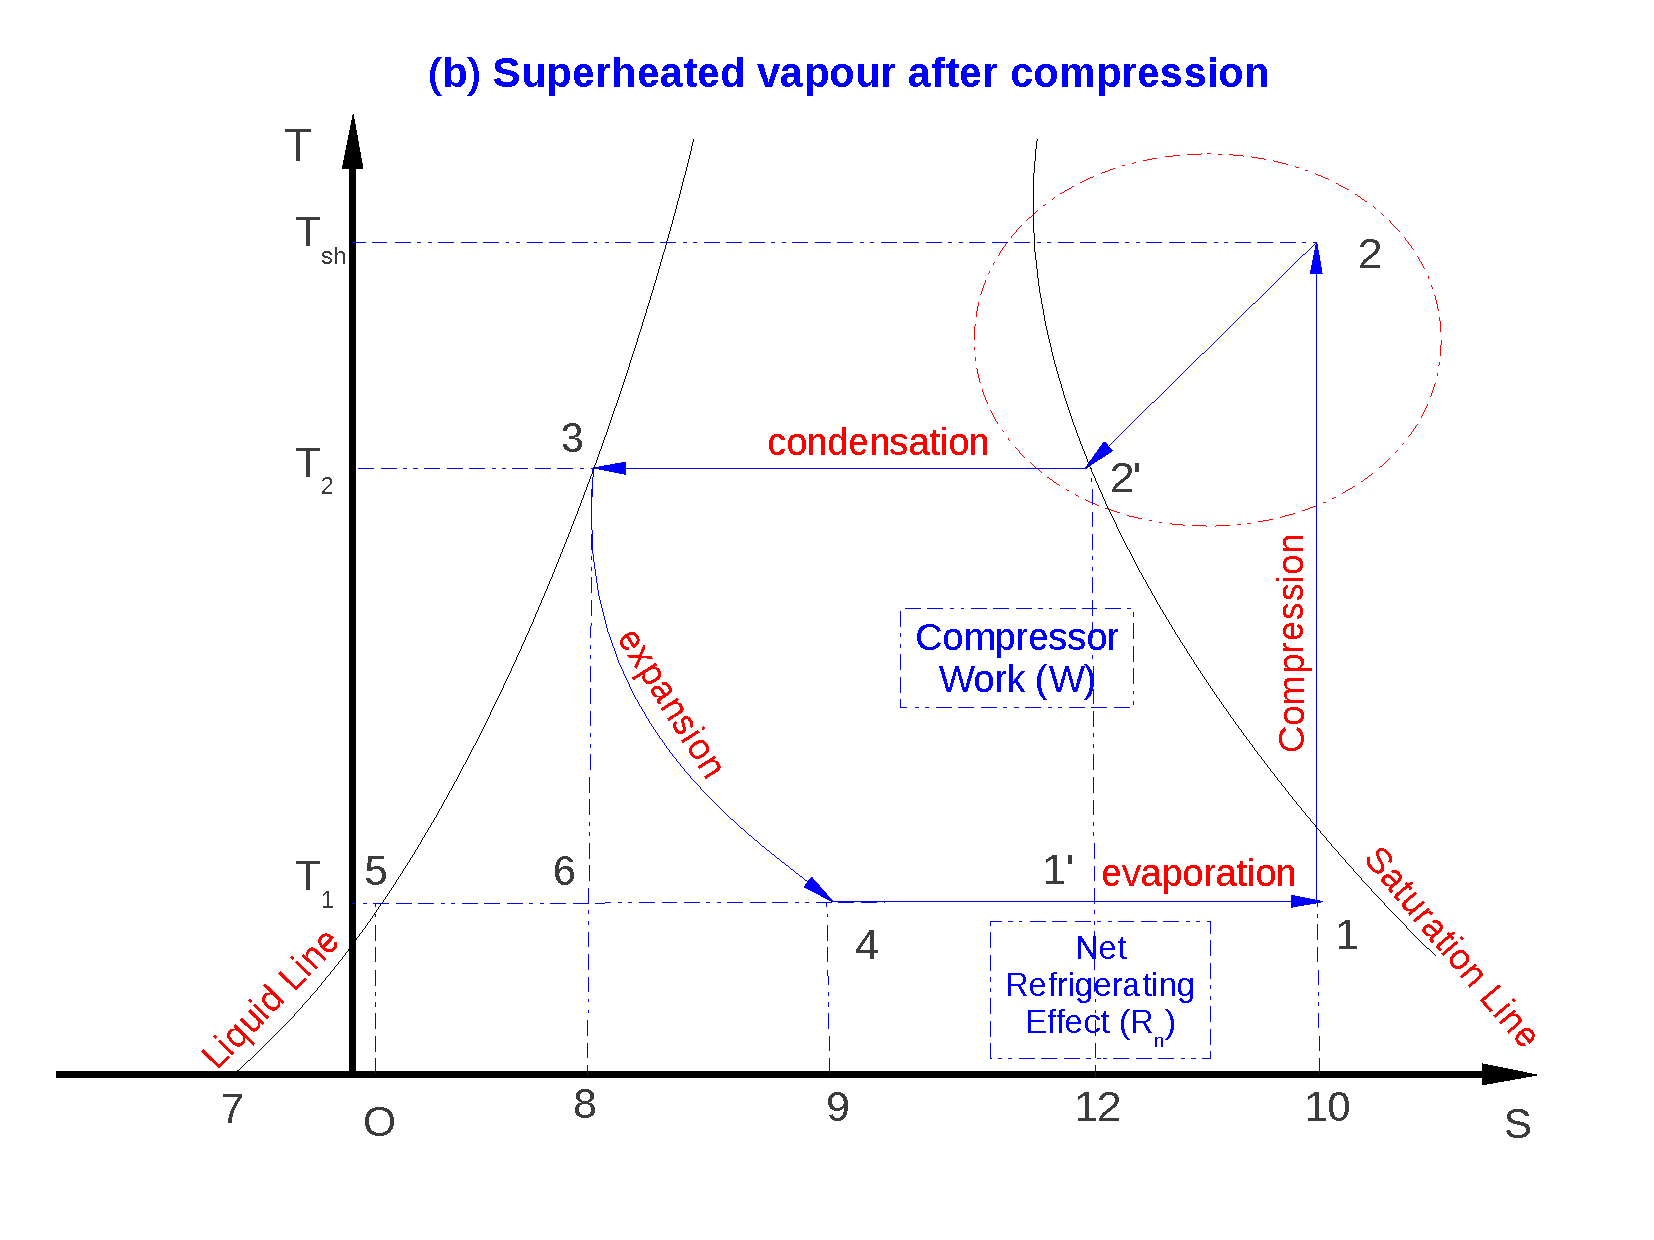
\includegraphics[width=4.cm,height=2.4cm,clip]{./Pics/Overview_Refrig15}
      \vspace{-.1cm}
      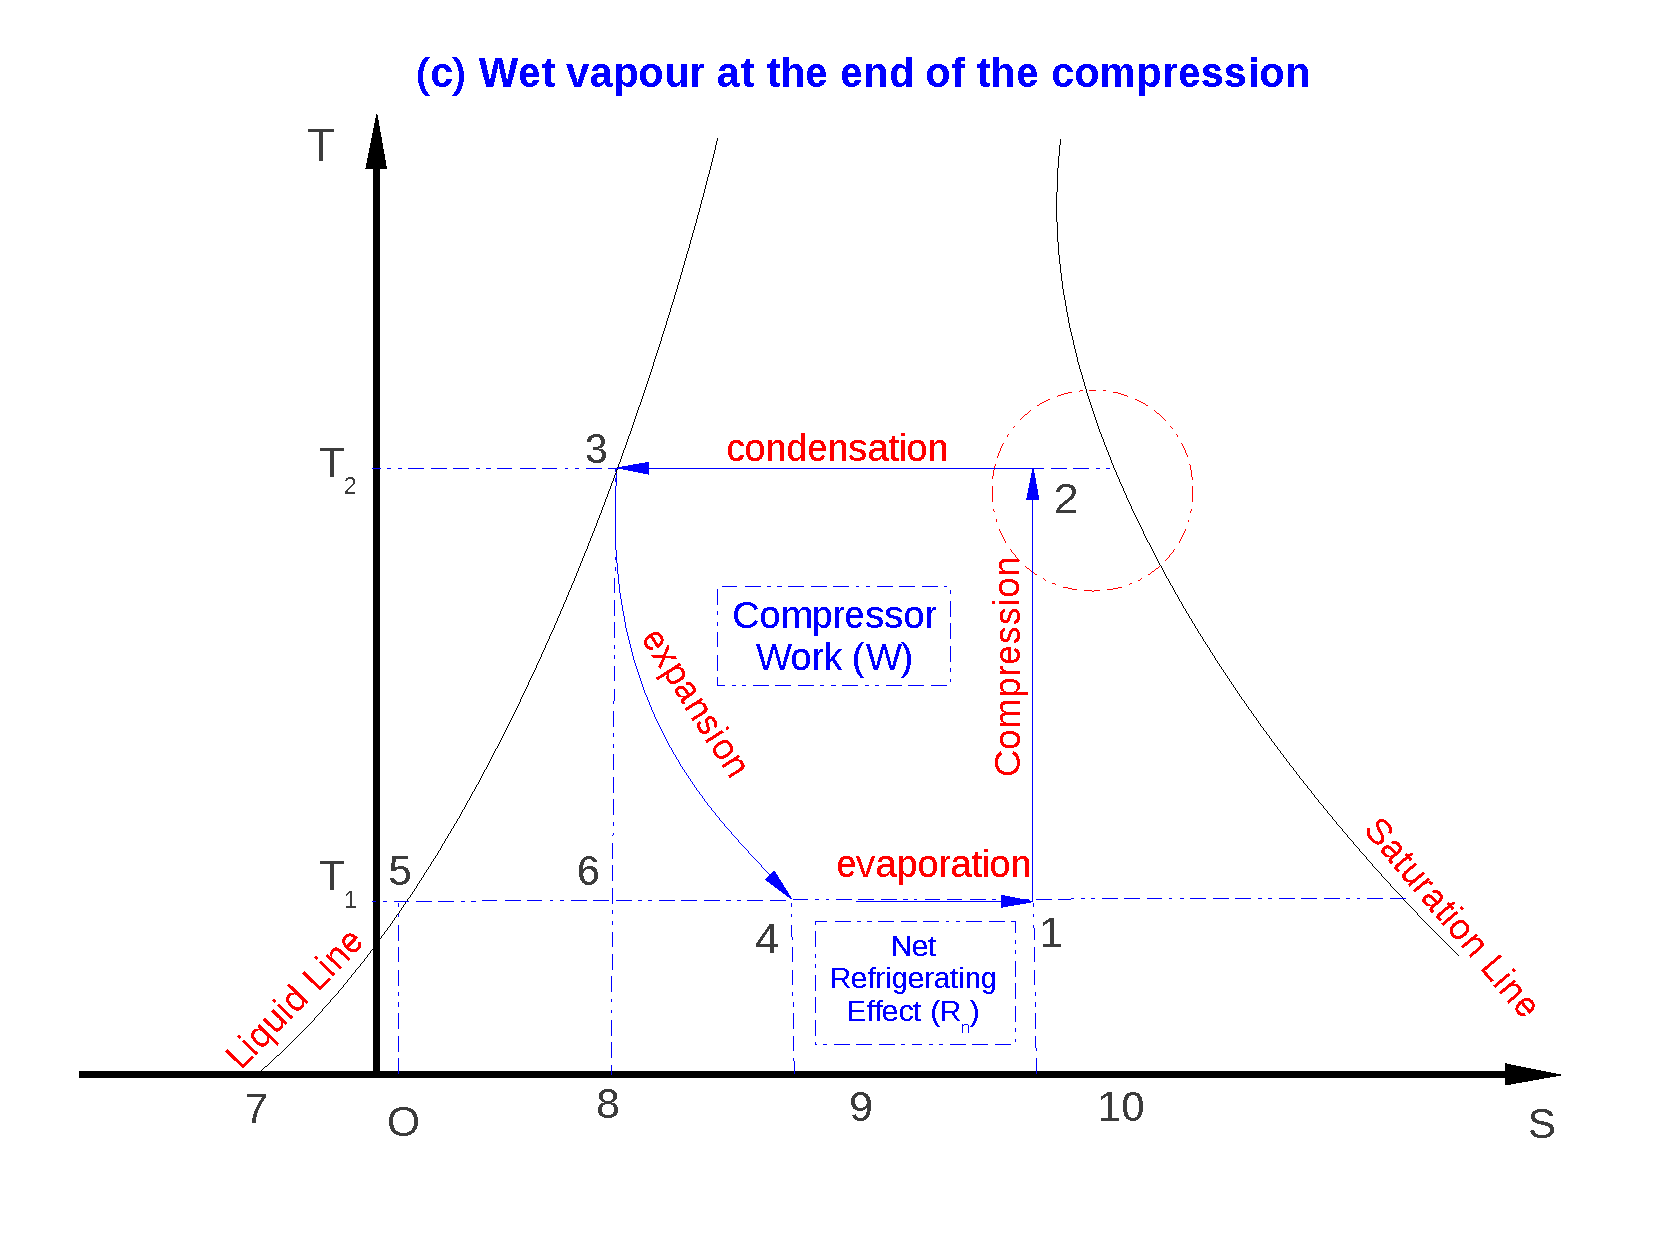
\includegraphics[width=4.cm,height=2.4cm,clip]{./Pics/Overview_Refrig16}}
   \end{figure}  
  \end{column}  
  \begin{column}[c]{0.45\linewidth}
   \begin{enumerate}[(a)]
    \item <1-> All processes of the refrigeration cycle are internally \textcolor{blue}{reversible}, \textcolor{blue}{except}; 
    \item <2-> The processes in the expansion valve which operate \textcolor{blue}{adiabatically};
    \item <3-> Refrigerant fluid that leaves the \textcolor{blue}{condenser} is \textcolor{blue}{saturated liquid}, whereas the fluid heading to the low pressure \textcolor{red}{compressor} is \textcolor{red}{saturated vapour}.
   \end{enumerate}
  \end{column}  
 \end{columns}
\end{frame}



%%%
%%% Slide
%%%
\begin{frame}
 \frametitle{Thermal Analysis -- $PH$ Diagram}
   \begin{figure}%
     \vbox{
      \hbox{\hspace{.8cm}
      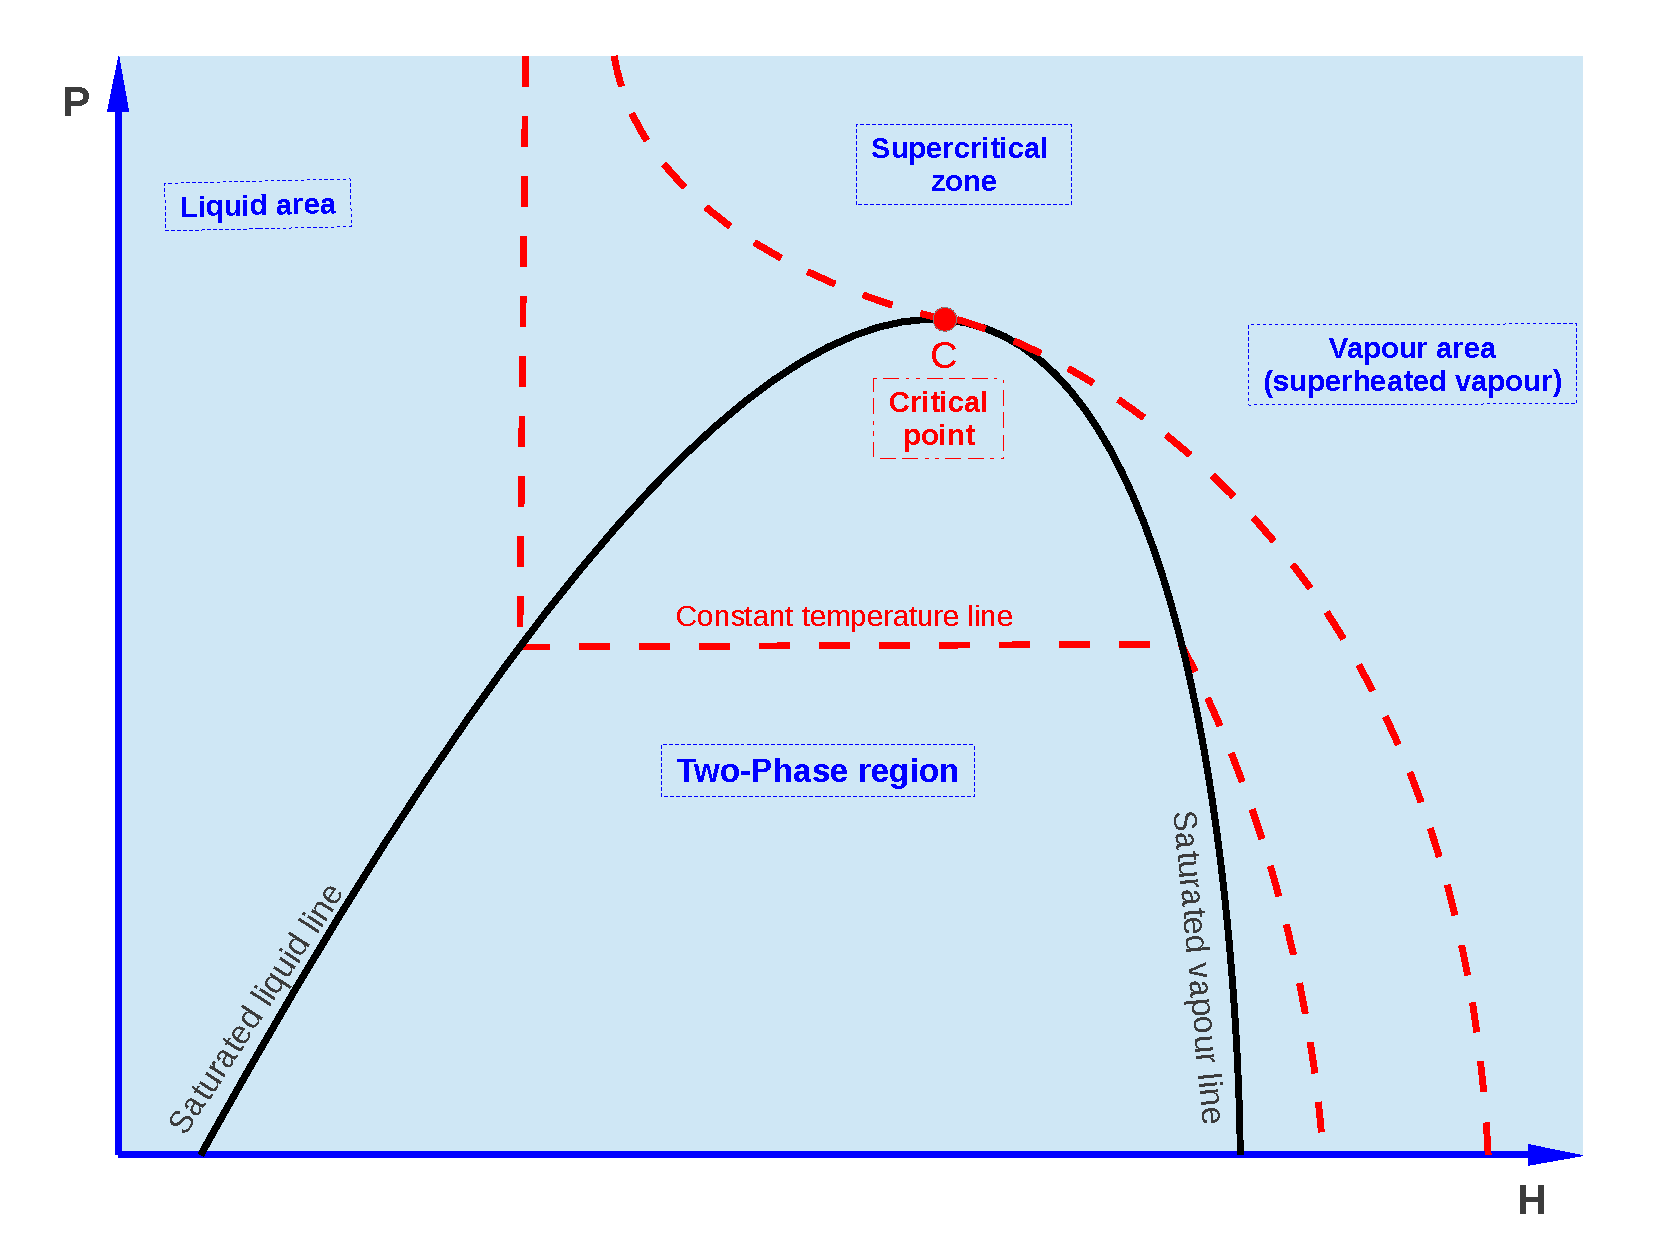
\includegraphics[width=4.6cm,height=3.8cm,clip]{./Pics/Overview_Refrig18}
      \hspace{.1cm}
      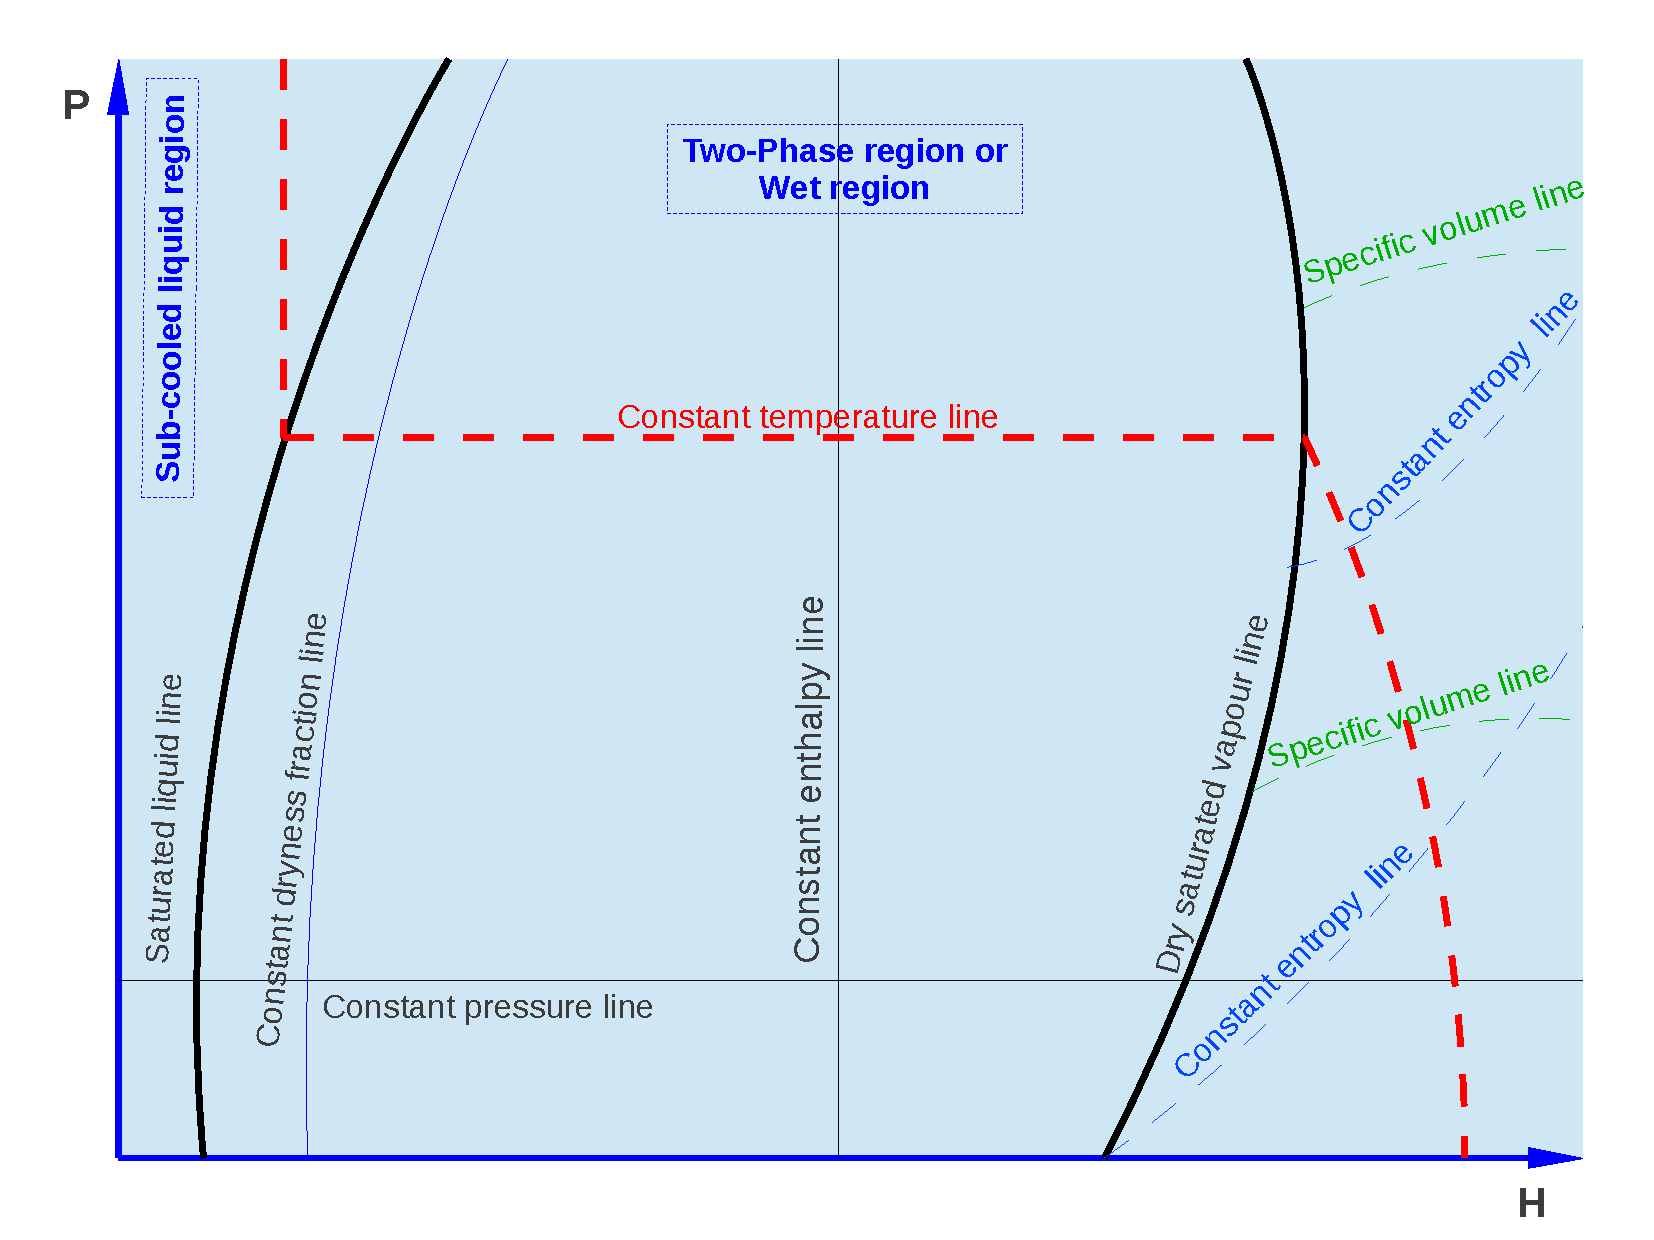
\includegraphics[width=4.6cm,height=3.8cm,clip]{./Pics/Overview_Refrig17}}
      \vspace{-.1cm}
      \hbox{\hspace{.8cm}
      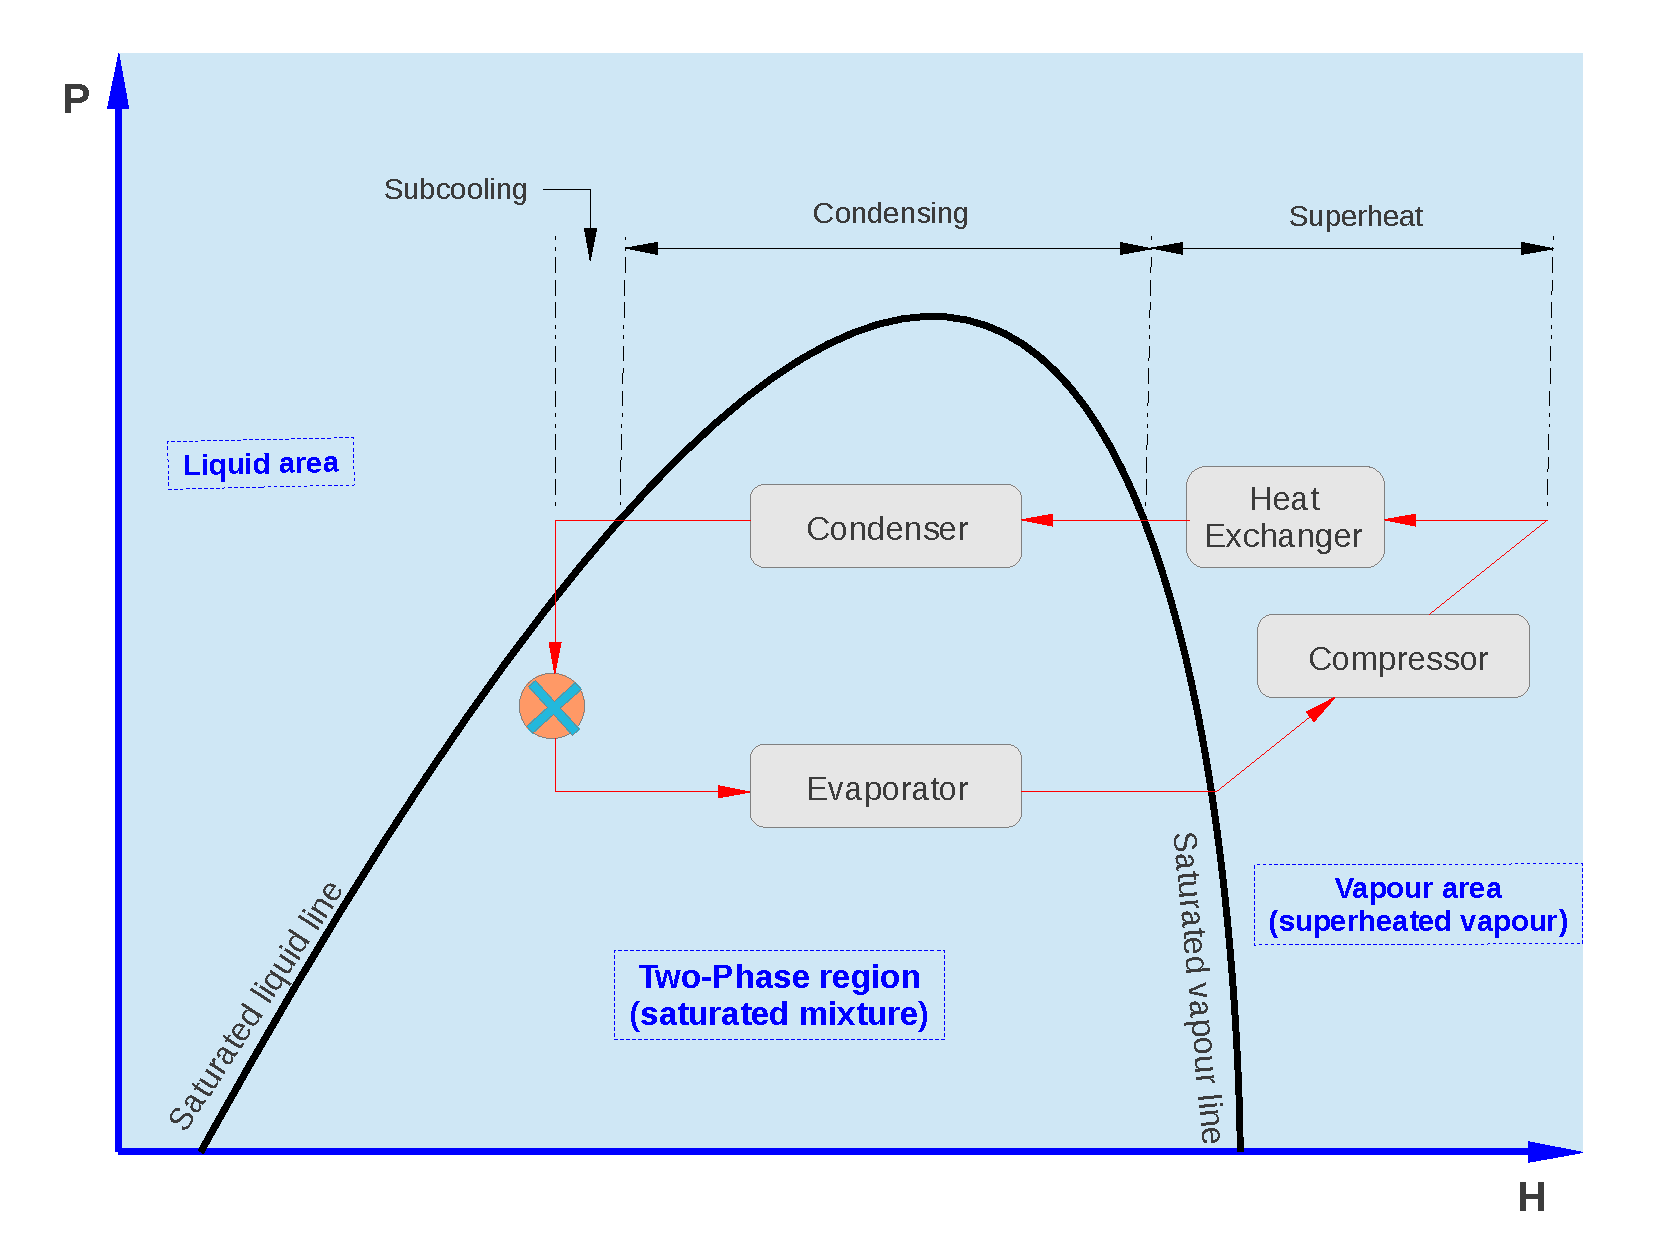
\includegraphics[width=4.6cm,height=3.87cm,clip]{./Pics/Overview_Refrig19}
      \hspace{.1cm}
      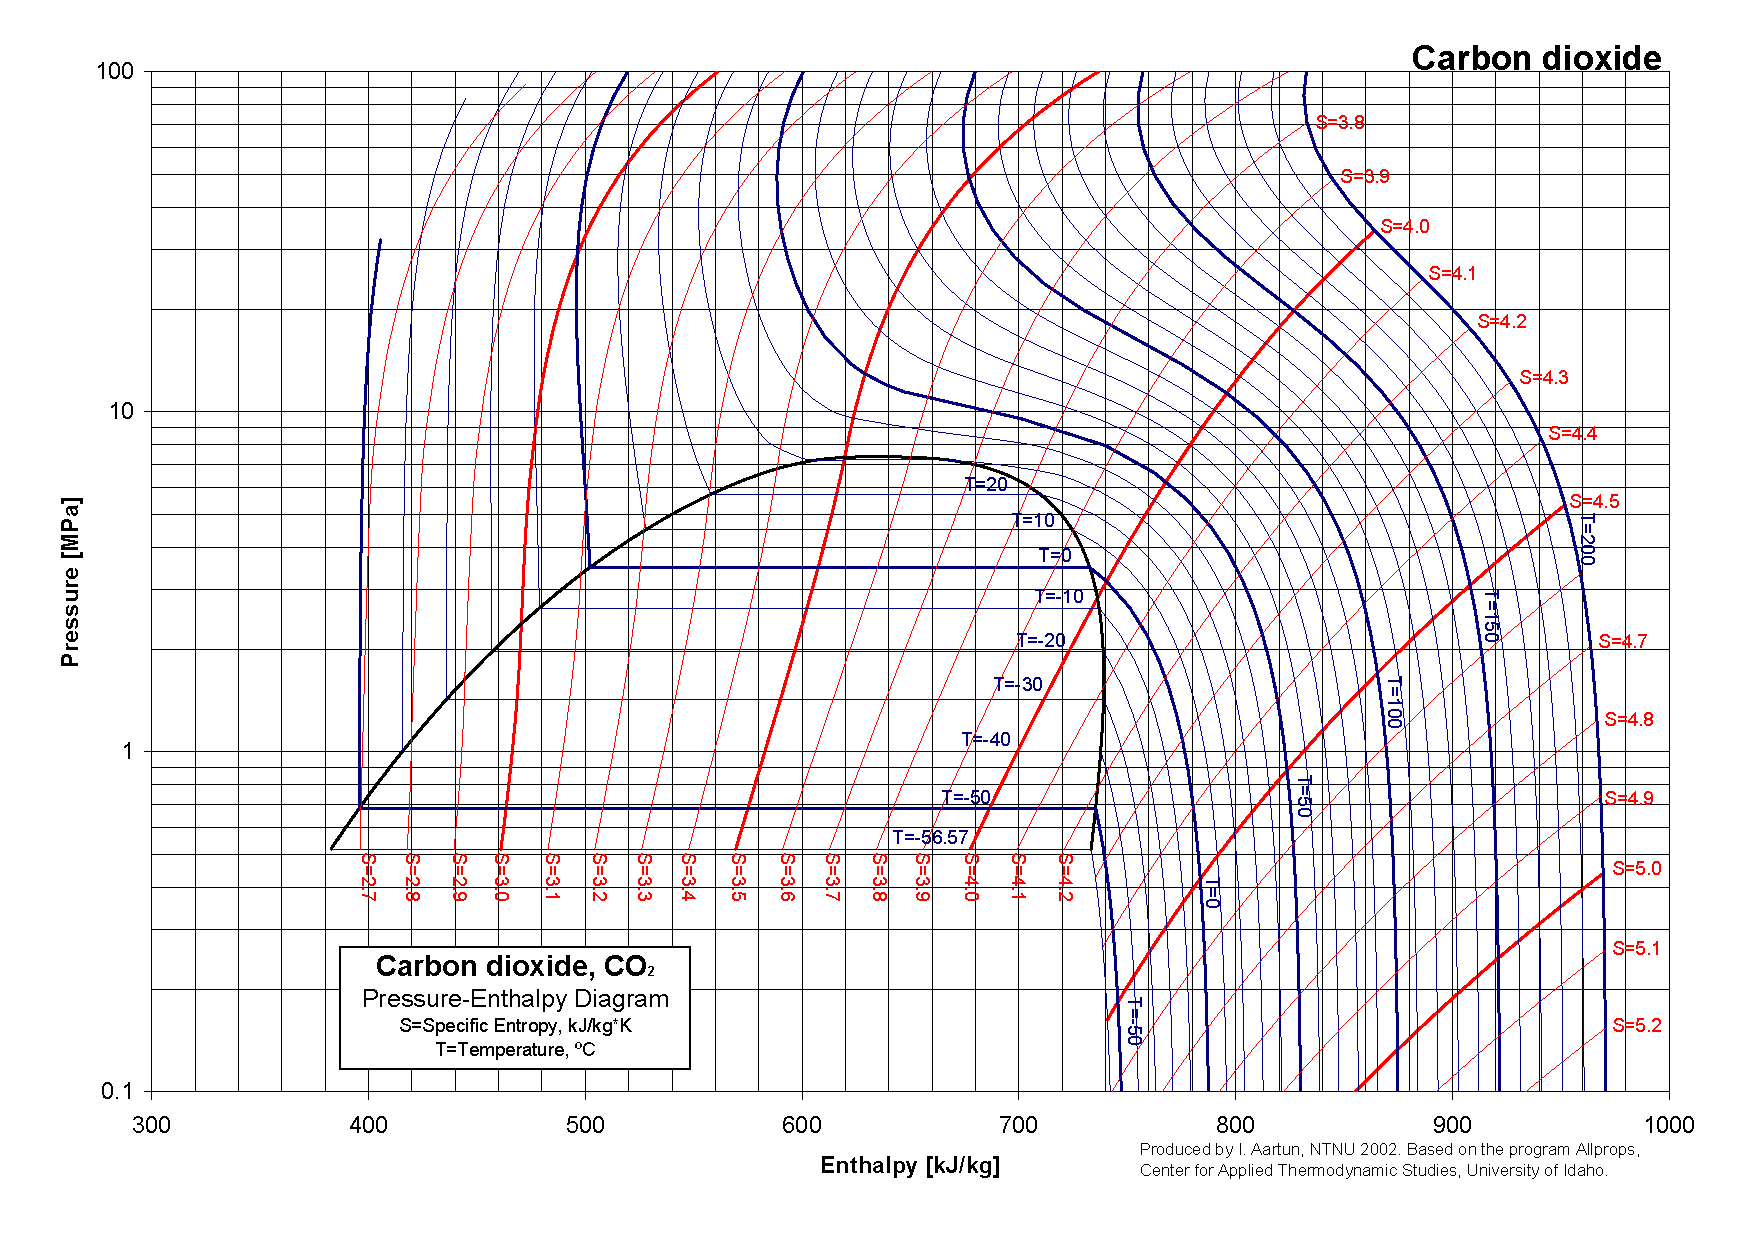
\includegraphics[width=4.9cm,height=4.cm,clip]{./Pics/CO2col}}}
   \end{figure}
\end{frame}


%%%
%%% SUBSECTION
%%%
\subsection{Multi-Pressure Systems}


%%%
%%% Slide
%%%
\begin{frame}
 \frametitle{Multi-Pressure Systems}
 \begin{columns}
  \begin{column}[c]{0.33\linewidth}
   \begin{figure}%
      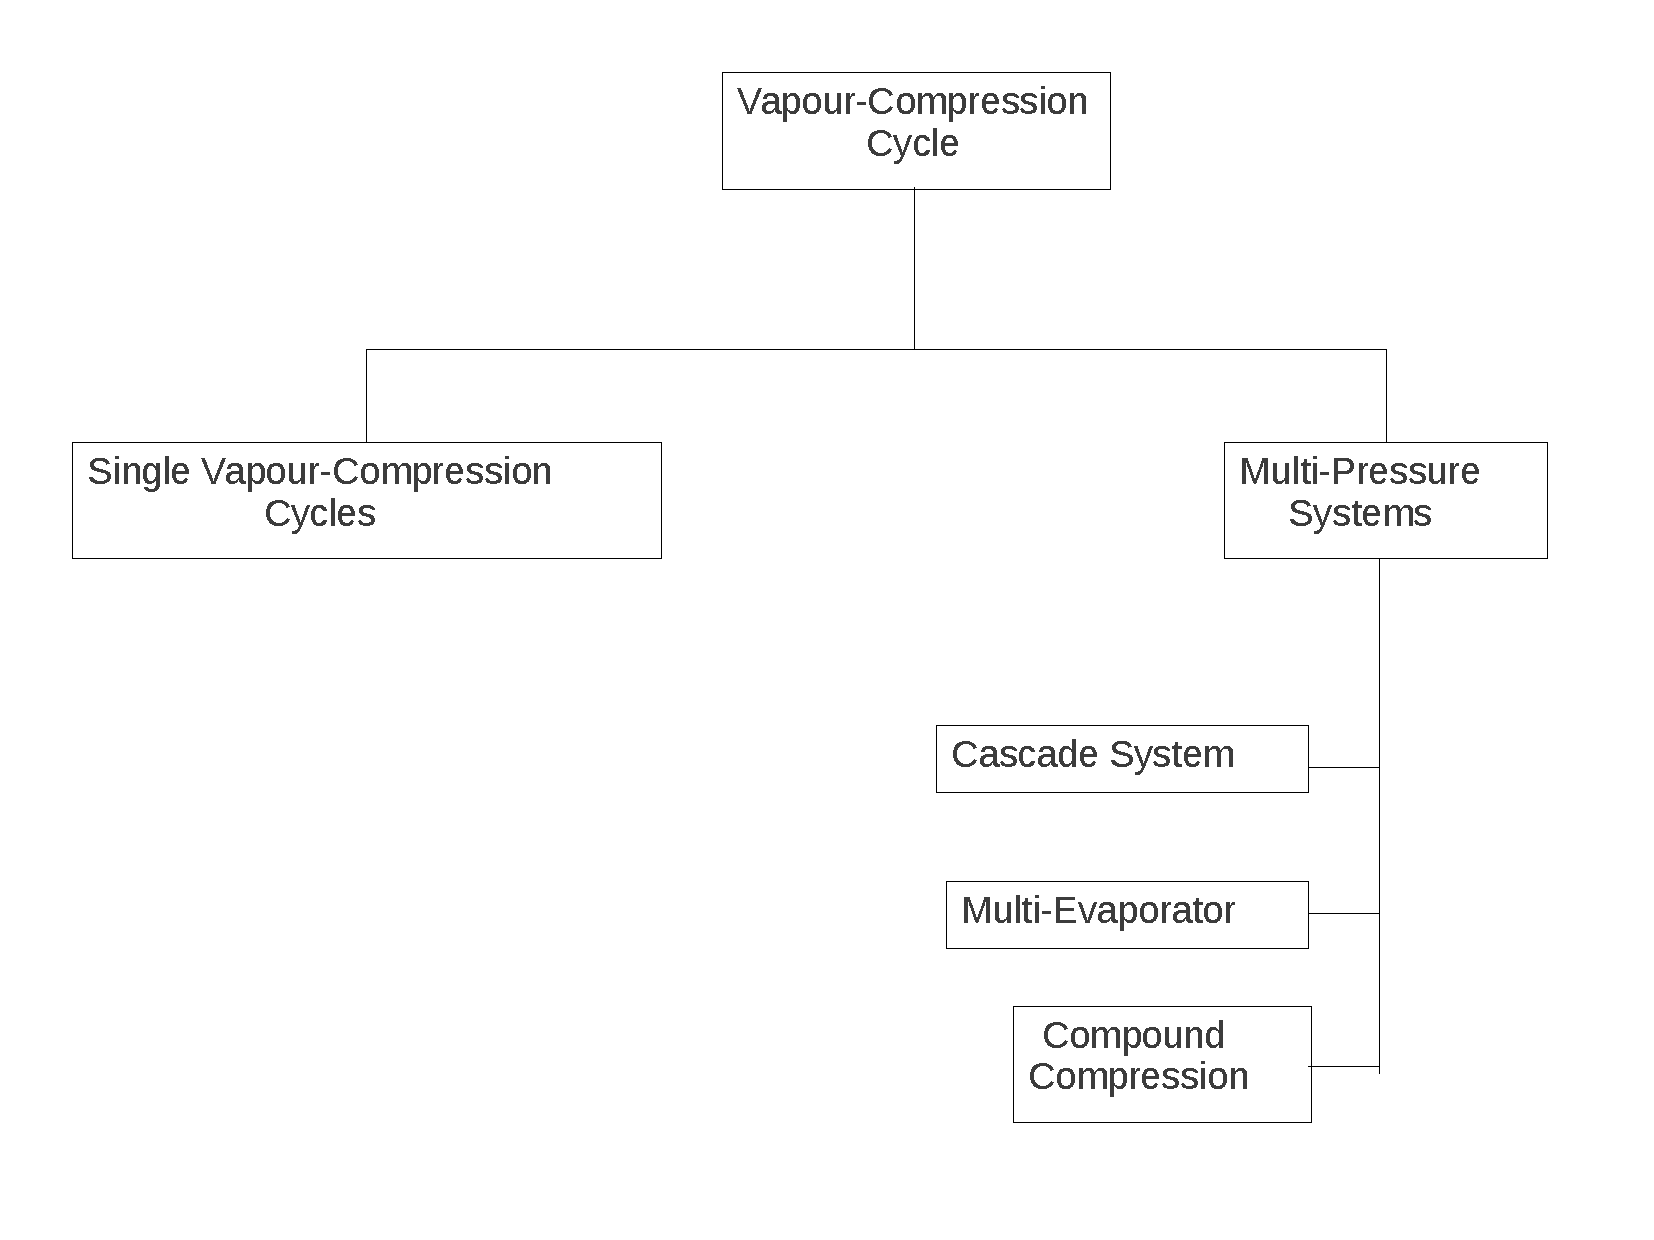
\includegraphics[width=4.5cm,height=4.5cm,clip]{./Pics/Overview_Refrig28}
   \end{figure}  
  \end{column}  
  \begin{column}[c]{0.67\linewidth}
   \begin{enumerate}[(a)]
    \item <1-> Multi-Pressure system is a refrigeration system that has 2 or more pressure levels;
    \item <2-> Some industrial processes require 2 or more temperature levels in the facility. This could be achieved with a set of individual single vapour-compression cycles however;
    \item <3-> The costs associated of such set of cycles may become prohibitive (too costy!);
    \item <4-> For high-condensing and low-evaporating temperature applications, a set of compressors is necessary due to the reduced volumetric efficiency;
    \item <5-> This issue can be overcomed by combining the set of compressors with intercooling;
    \item <6-> While in single-stage compression the lowest working temperature achieved is $\approx$ -30$^{\text{o}}$C, with 2- and 3-stage compression, the temperature may reach -55 and -80$^{\text{o}}$C, respectively.
   \end{enumerate} 
  \end{column}  
 \end{columns} 
\end{frame}


%%%
%%% Slide
%%%
\begin{frame}
 \frametitle{Multi-Stage Cascade Refrigeration}
 \begin{columns}
  \begin{column}[c]{0.45\linewidth}
   \begin{figure}%
     \vbox{
      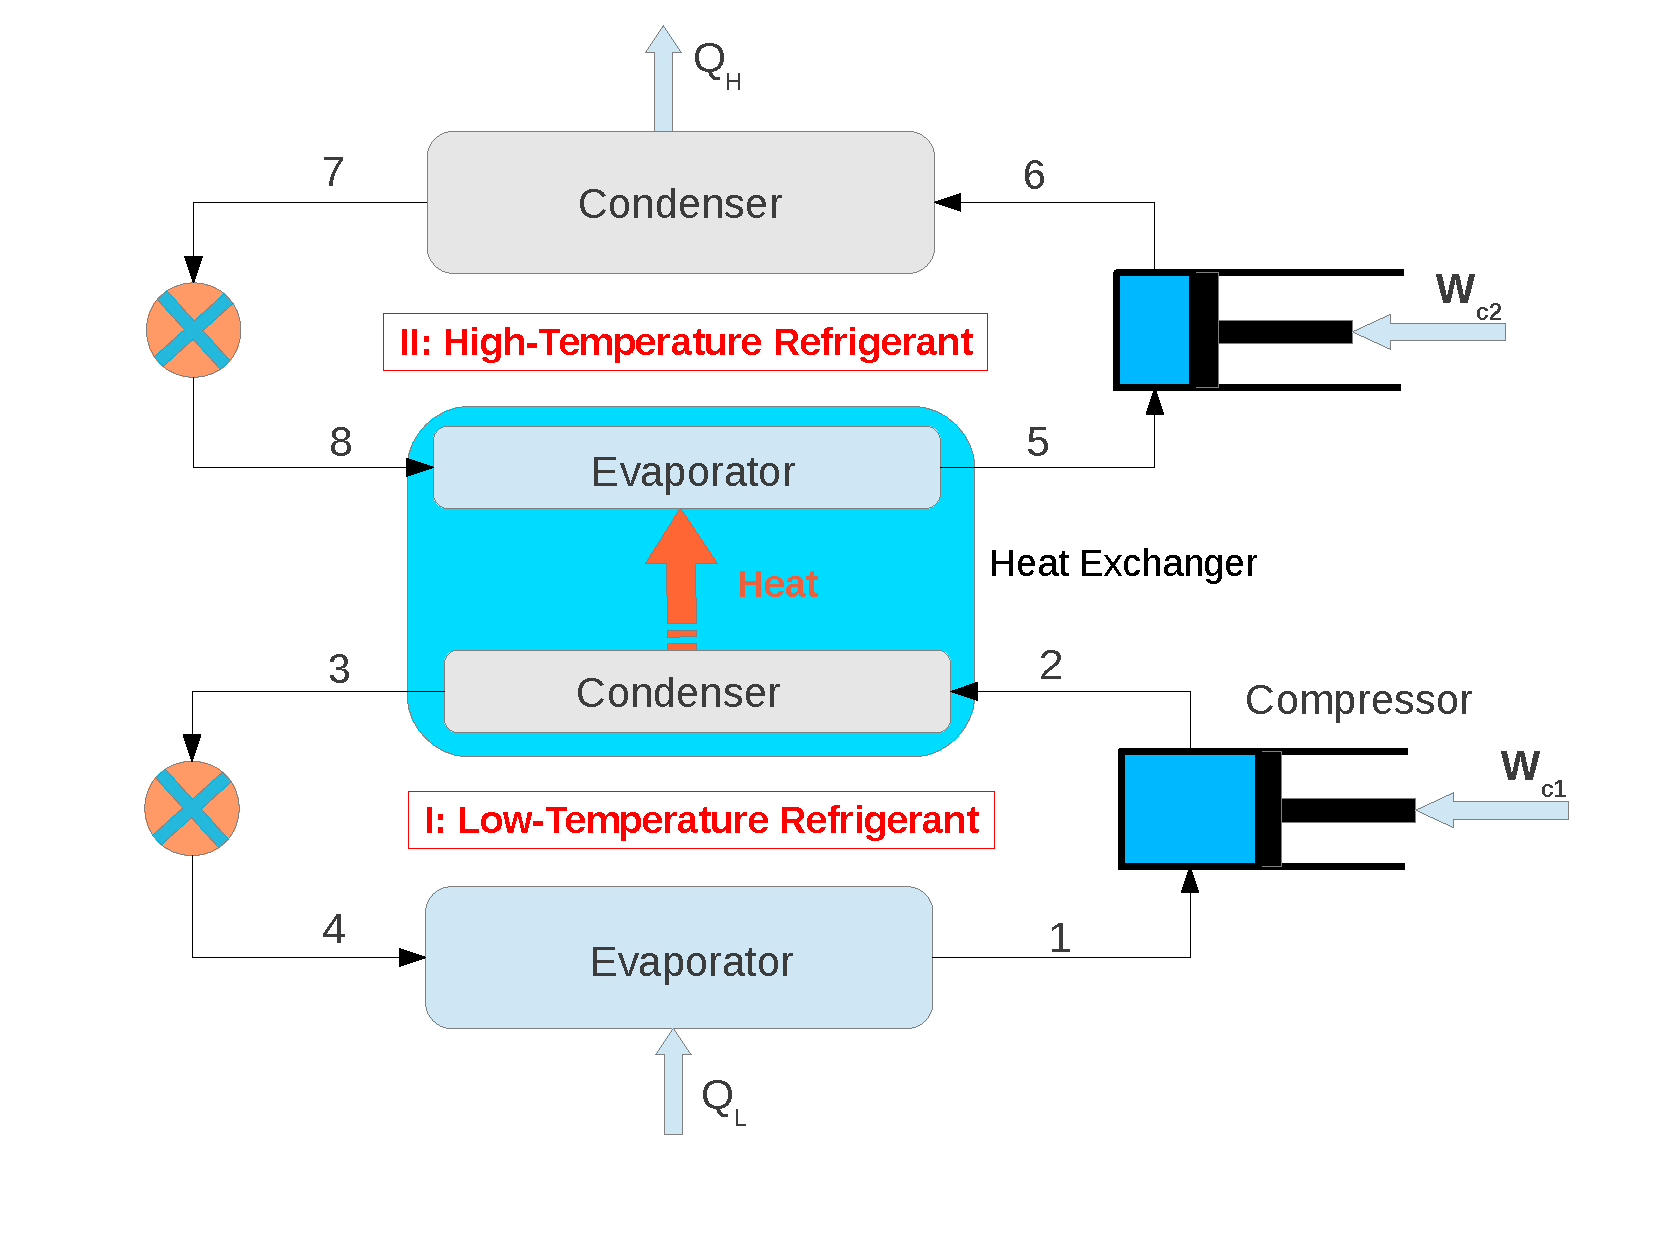
\includegraphics[width=4.5cm,height=3.5cm,clip]{./Pics/Overview_Refrig24}
      \vspace{-.1cm}
      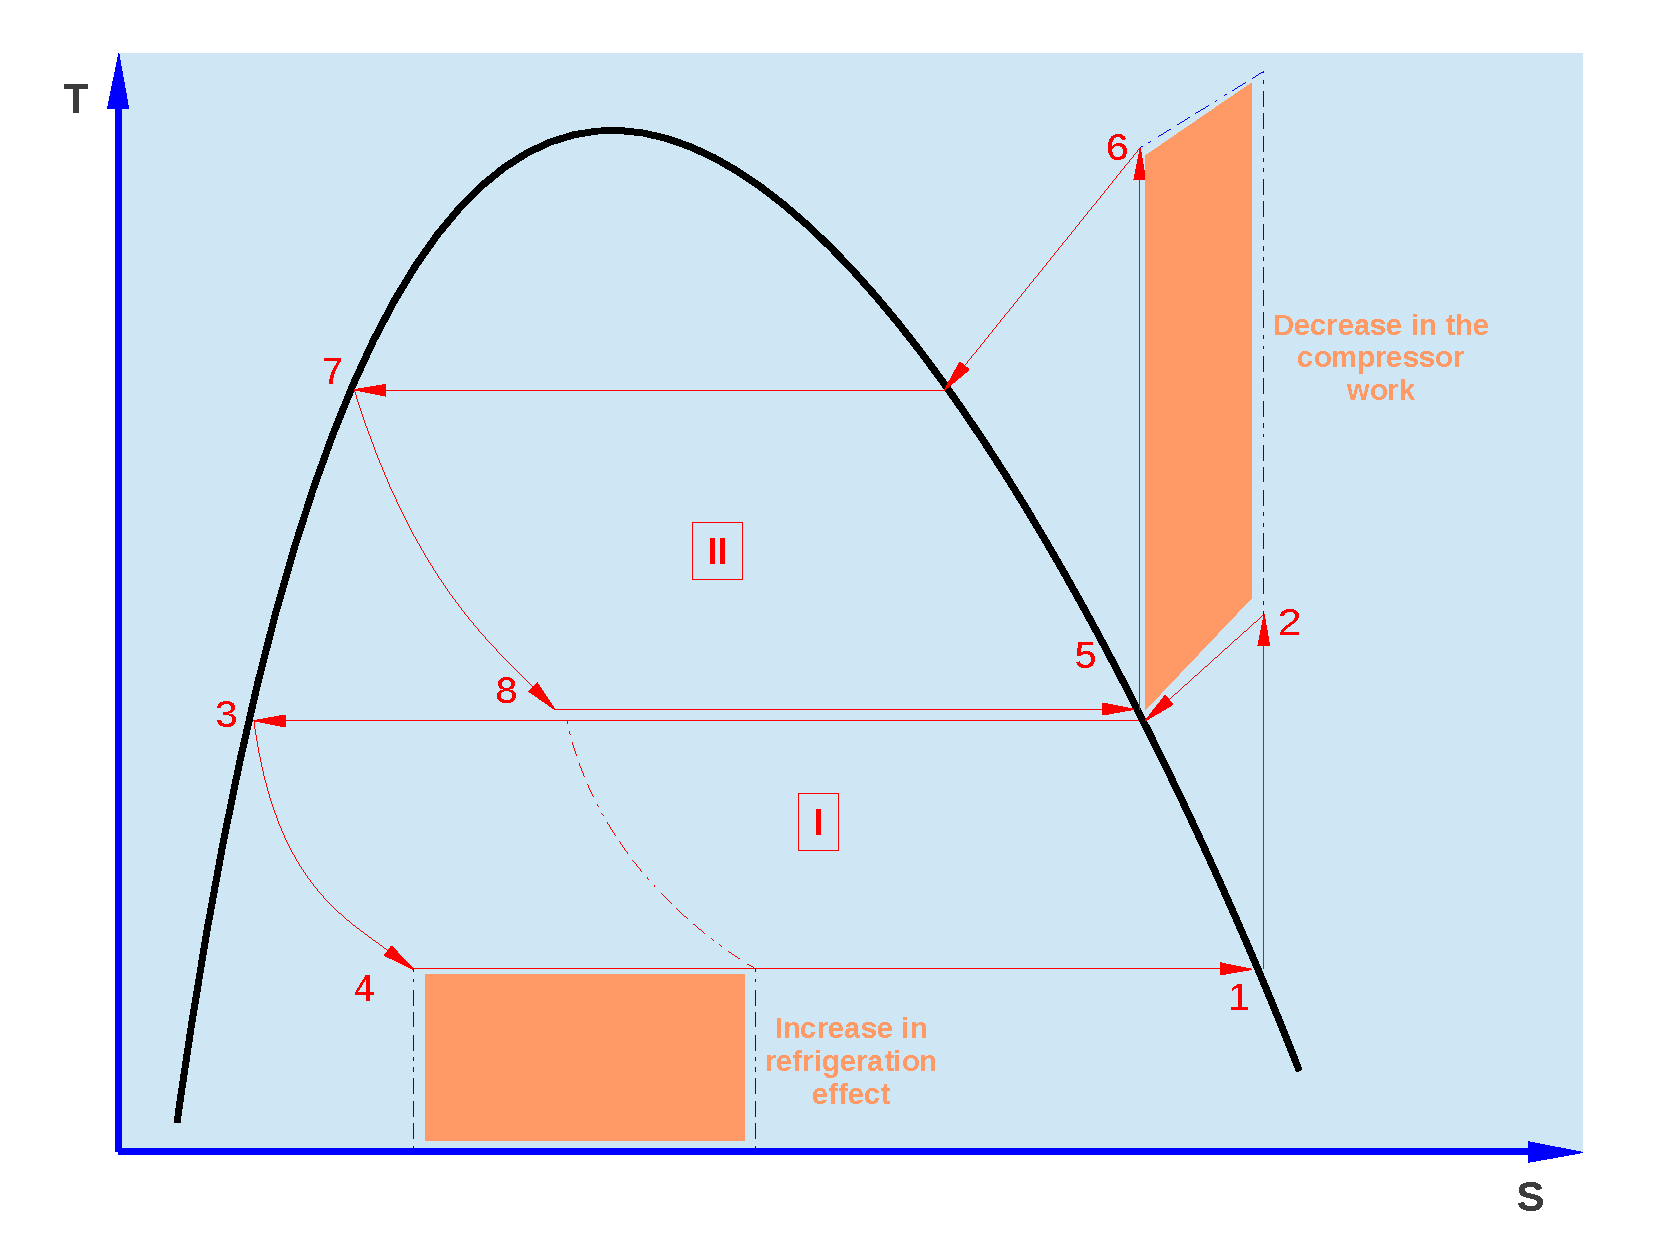
\includegraphics[width=4.cm,height=4.cm,clip]{./Pics/Overview_Refrig25}}
   \end{figure}  
  \end{column}  
  \begin{column}[c]{0.55\linewidth}
   \begin{enumerate}[(a)]
    \item <1-> Simple vapour-compression refrigeration cycles are inexpensive and reliable however for large industrial systems \textcolor{blue}{efficiency} is a major requirement;
    \item <2-> Some industrial applications requires large temperature range which leads to large pressure range (and therefore low performance/efficiency in the compressor);
    \item <3-> Similar to the vapour thermal systems, we can improve the efficiency of the cycle by coupling two (or more) cycles (in parallel) through heat exchangers that will operate simultaneously as evaporator and condenser;
   \end{enumerate} 
  \end{column}  
 \end{columns} 
\end{frame}


%%%
%%% Slide
%%%
\begin{frame}
 \frametitle{Multi-Stage Cascade Refrigeration}
 \begin{columns}
  \begin{column}[c]{0.45\linewidth}
   \begin{figure}%
     \vbox{
      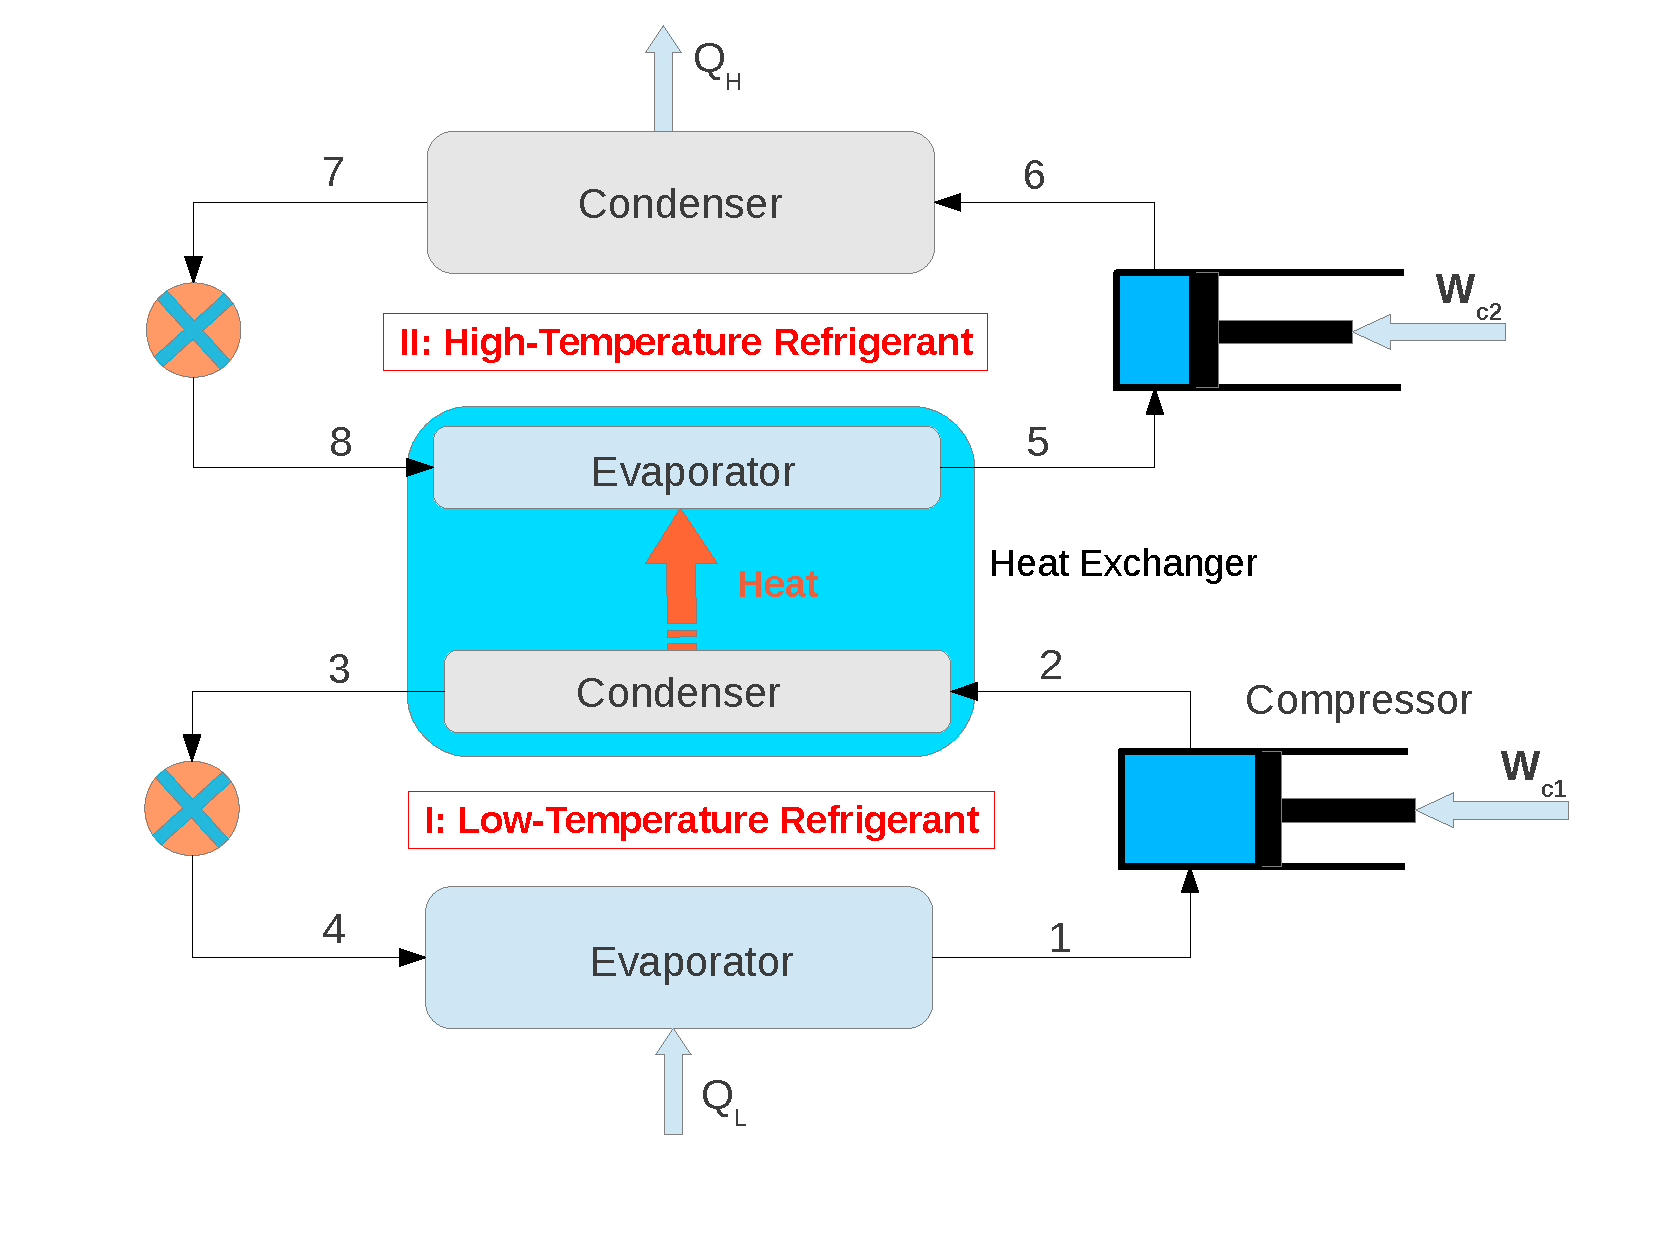
\includegraphics[width=4.5cm,height=3.5cm,clip]{./Pics/Overview_Refrig24}
      \vspace{-.1cm}
      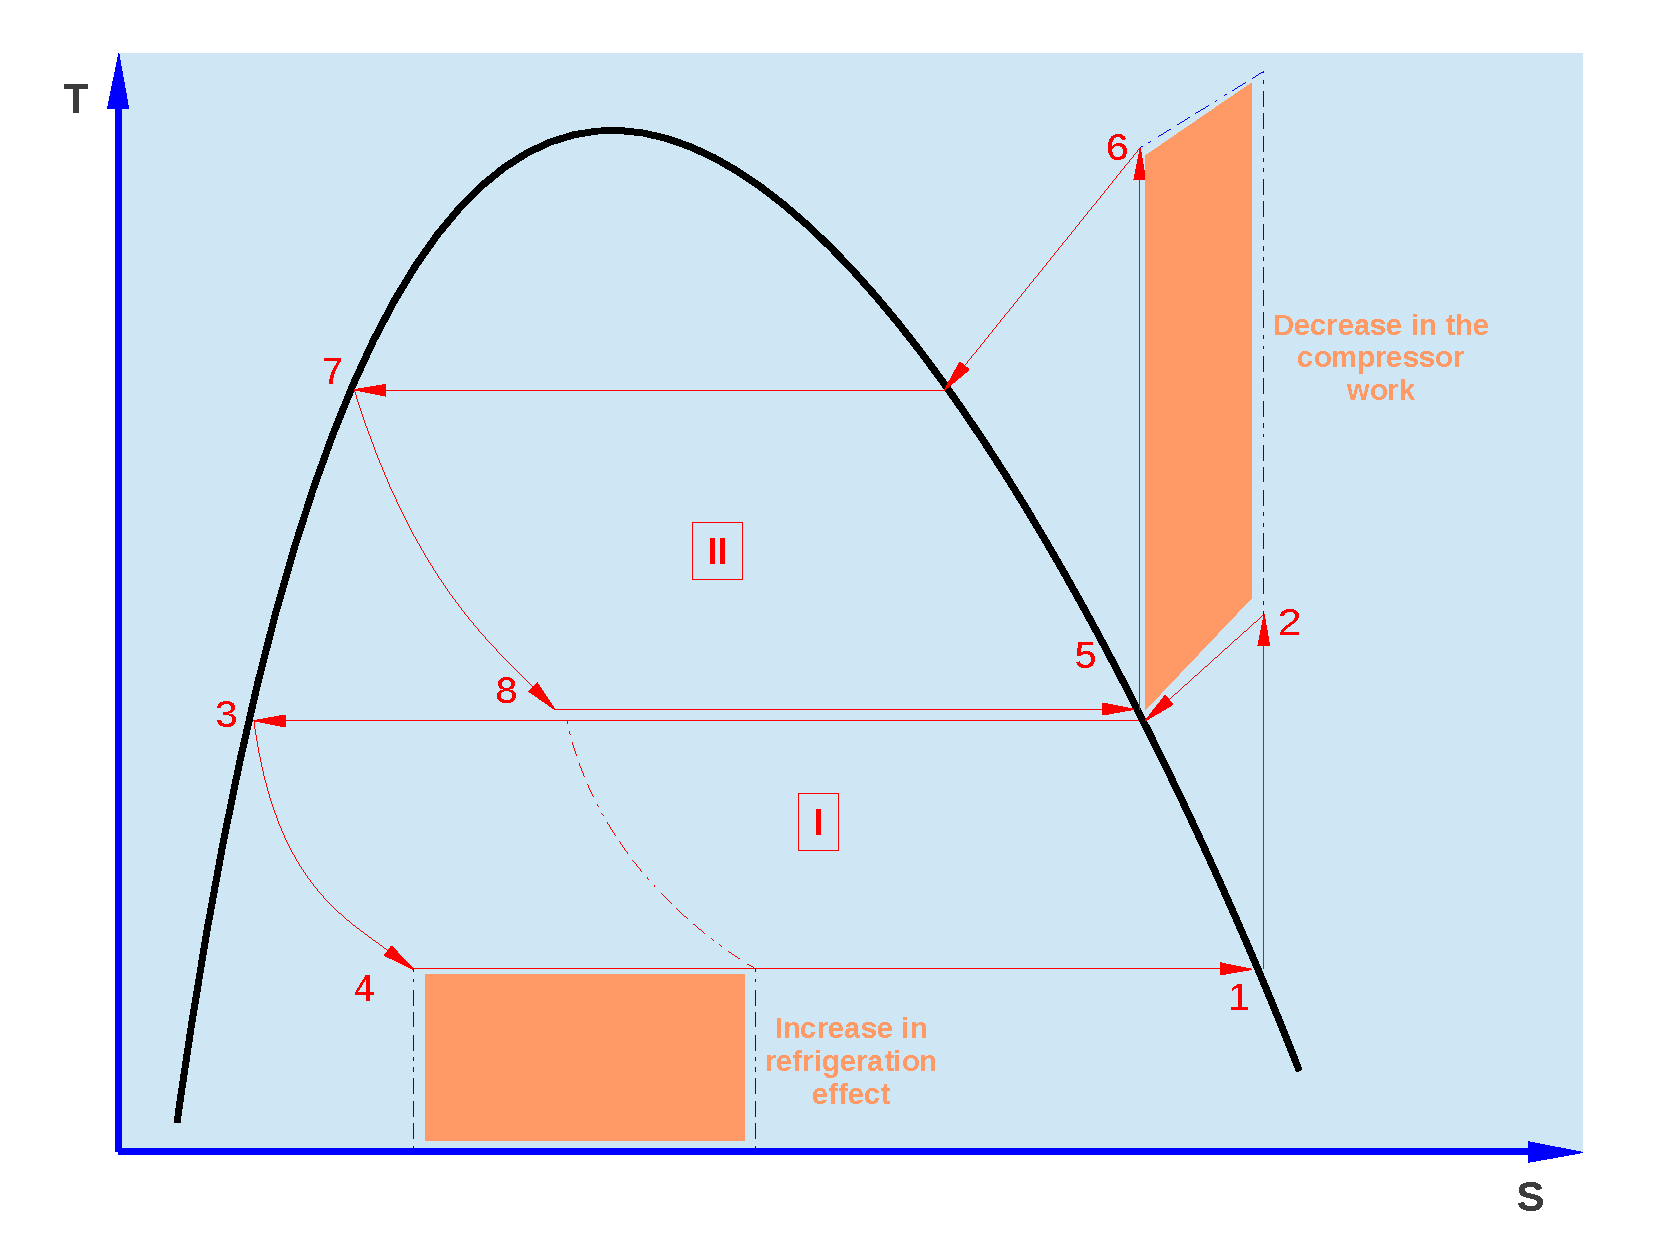
\includegraphics[width=4.cm,height=4.cm,clip]{./Pics/Overview_Refrig25}}
   \end{figure}  
  \end{column}  
  \begin{column}[c]{0.55\linewidth}
   \begin{enumerate}[(a)]\setcounter{enumi}{3}
    \item <1-> The number of stages depends only on the required temperature range;
    \item <2-> The refrigerant fluid will also depend upon the required temperature and thus 2 or more fluids can be used as they do not mix (i.e., mass-isolated cycles).
   \end{enumerate}
  \end{column}  
 \end{columns} 
\end{frame}



%%%
%%% Slide
%%%
\begin{frame}
 \frametitle{Multi-Stage Compression with Intercooling Refrigeration}
 \begin{columns}
  \begin{column}[c]{0.45\linewidth}
   \begin{figure}%
     \vbox{
      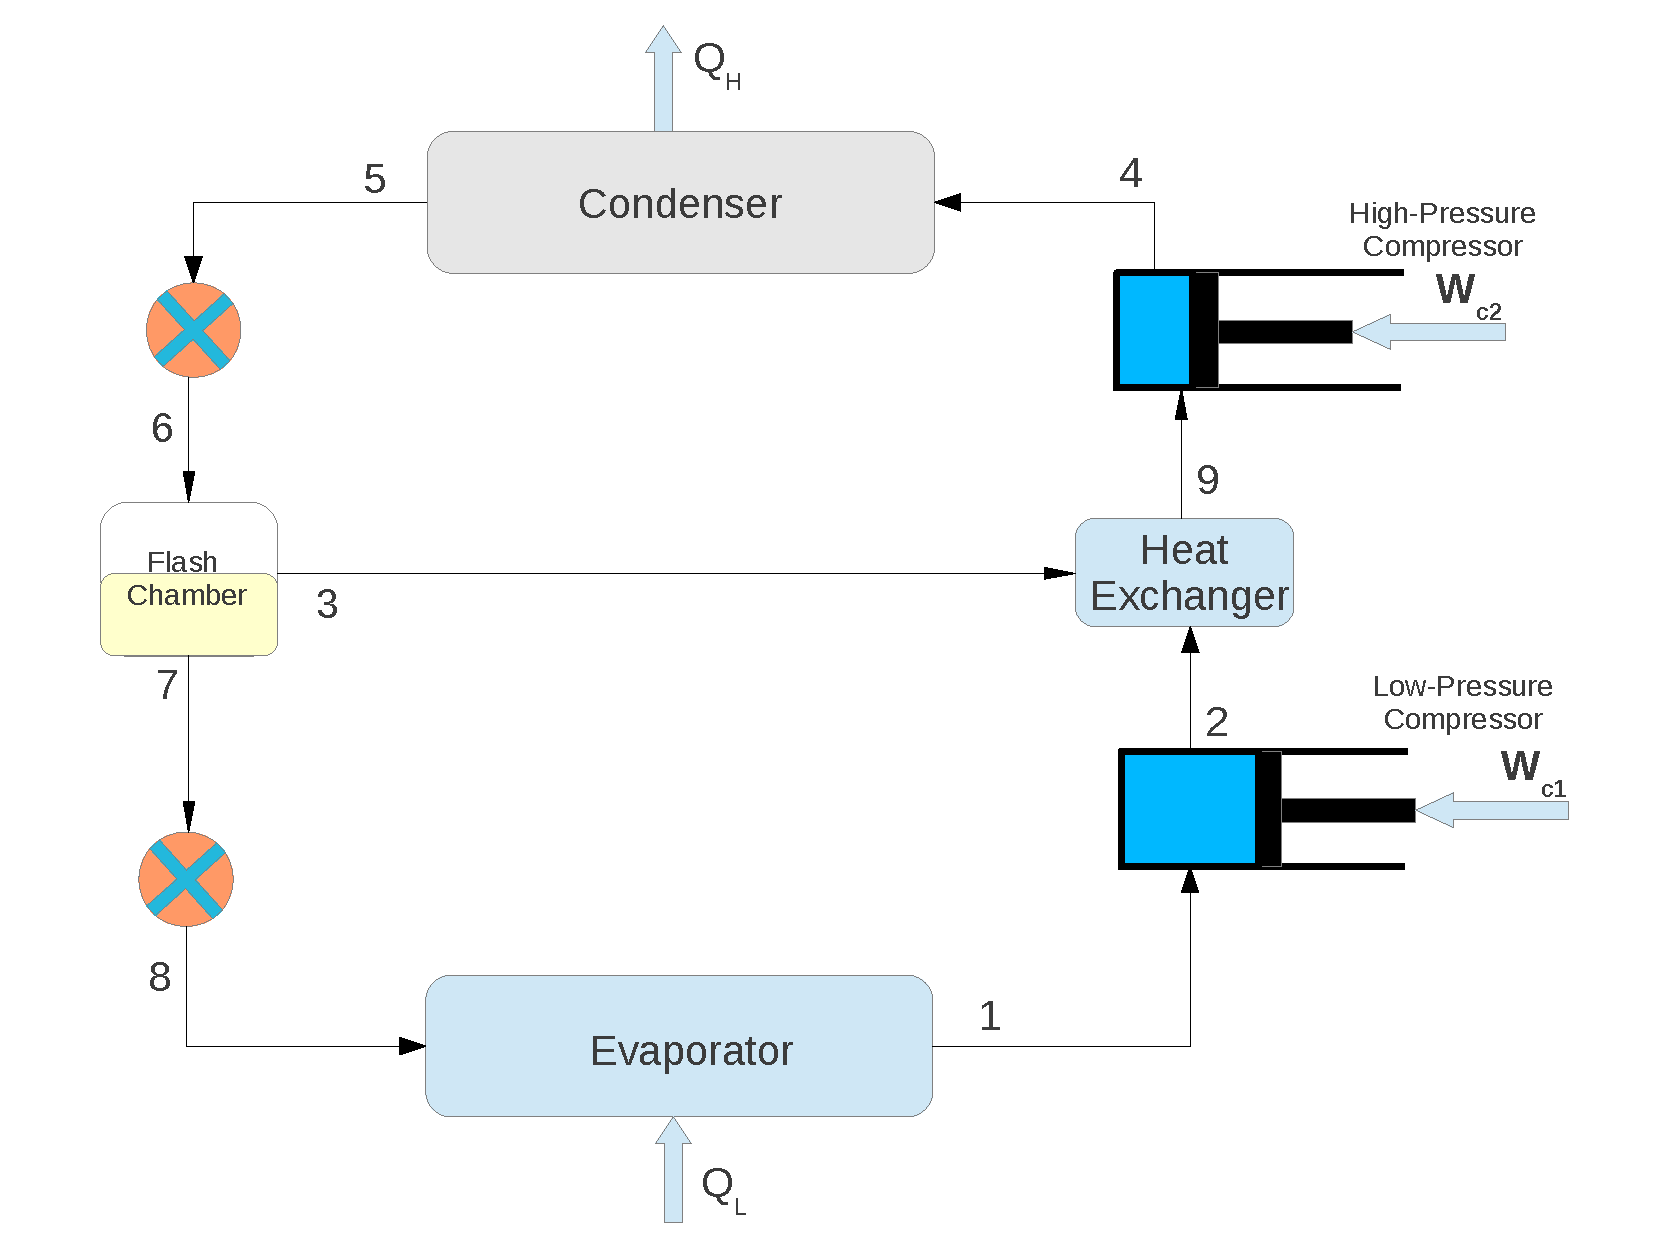
\includegraphics[width=4.5cm,height=3.5cm,clip]{./Pics/Overview_Refrig26}
      \vspace{-.1cm}
      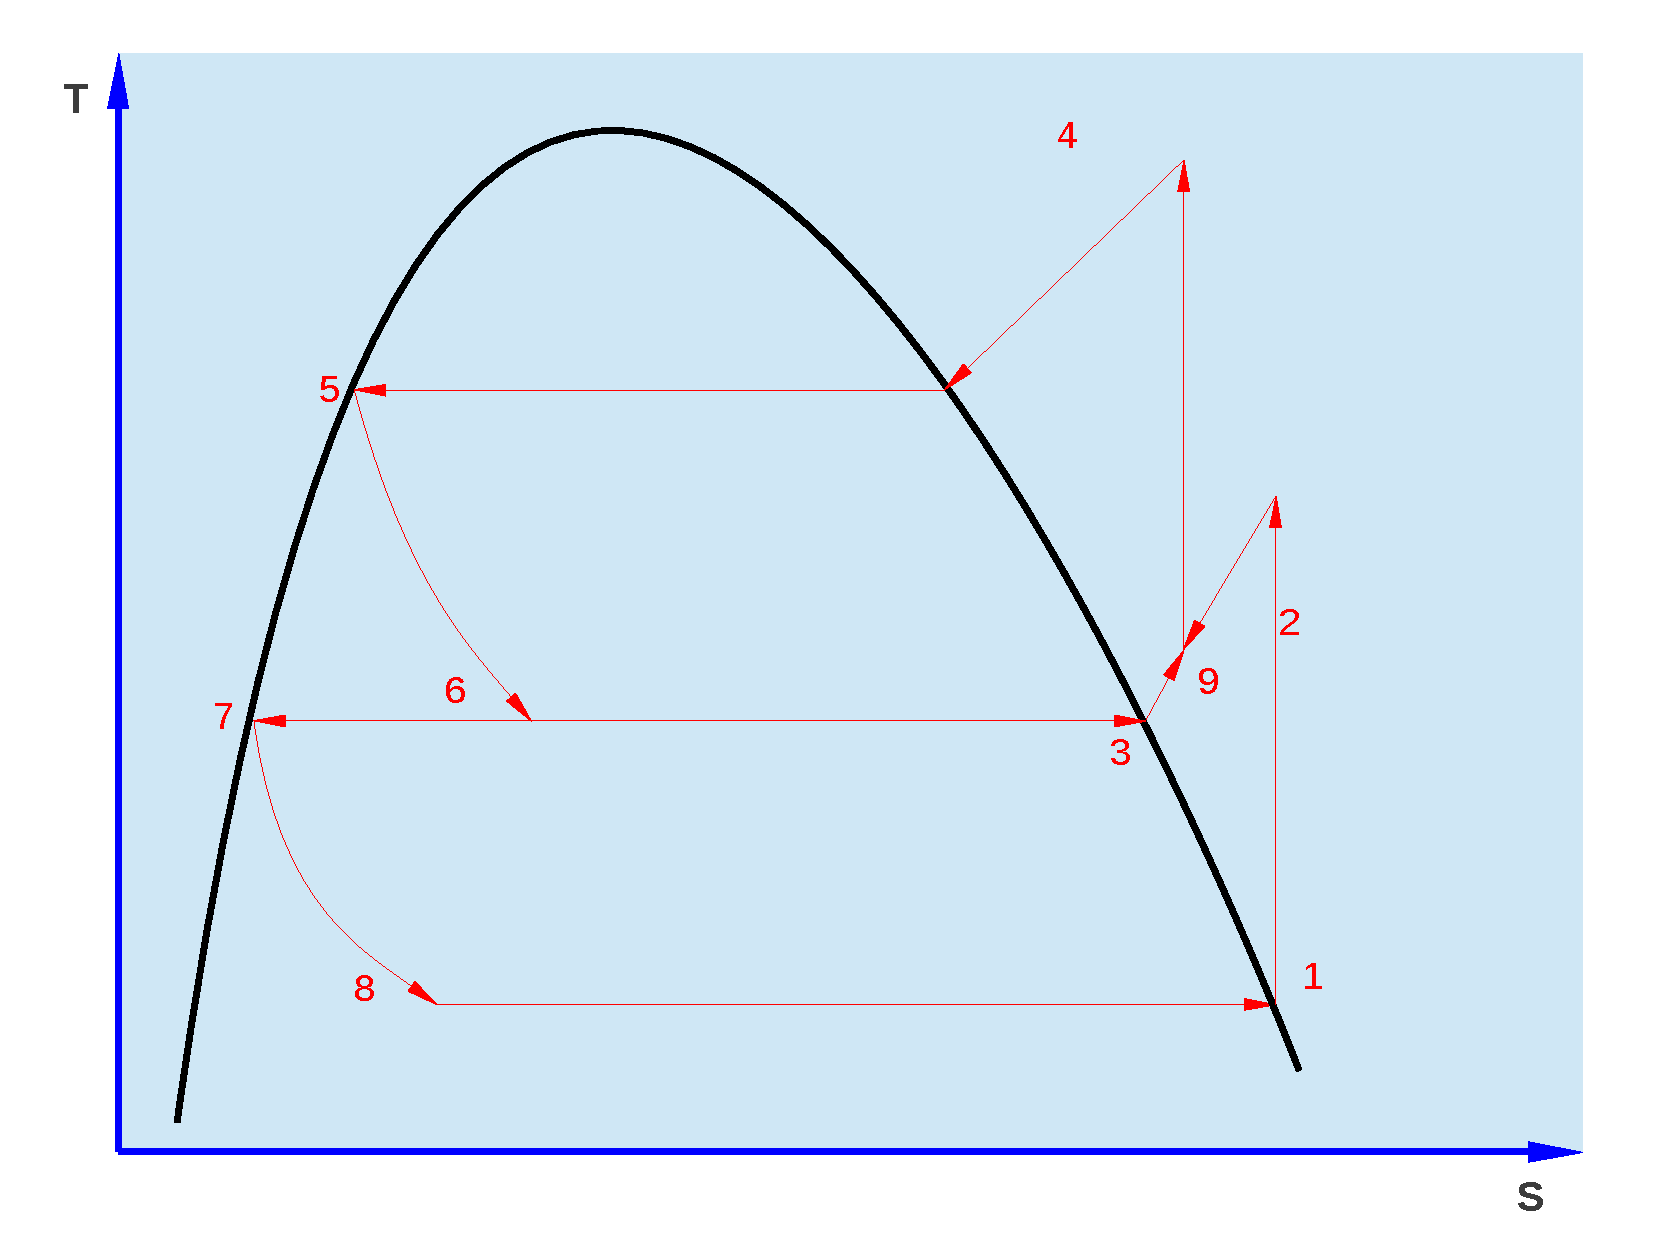
\includegraphics[width=4.cm,height=4.cm,clip]{./Pics/Overview_Refrig27}}
   \end{figure}  
  \end{column}  
  \begin{column}[c]{0.55\linewidth}
   \begin{enumerate}[(a)]
    \item <1-> This special and complex process is applied when the cascade refrigeration is used with \textcolor{blue}{a single refrigerant fluid};
    \item <2-> In this case, the heat exchanger is replaced by a \textcolor{blue}{{\it flash chamber}} (i.e., a liquid-vapour separator);
    \item <3-> The refrigerant is partially compressed in the LP stage (1-2);
    \item <4-> After leaving the LP compressor, the fluid is cooled by mixing with vapour stream from the flash chamber (3) in the intermediate heat exchanger to a temperature $T_{9}<T_{2}$;
    \item <5-> Such reduction of temperature results in smaller compressor work.
   \end{enumerate}
  \end{column}  
 \end{columns} 
\end{frame}


%%%
%%% Slide
%%%
\begin{frame}
 \frametitle{Multi-Stage Compression with Intercooling Refrigeration}
 \begin{columns}
  \begin{column}[c]{0.45\linewidth}
   \begin{figure}%
     \vbox{
      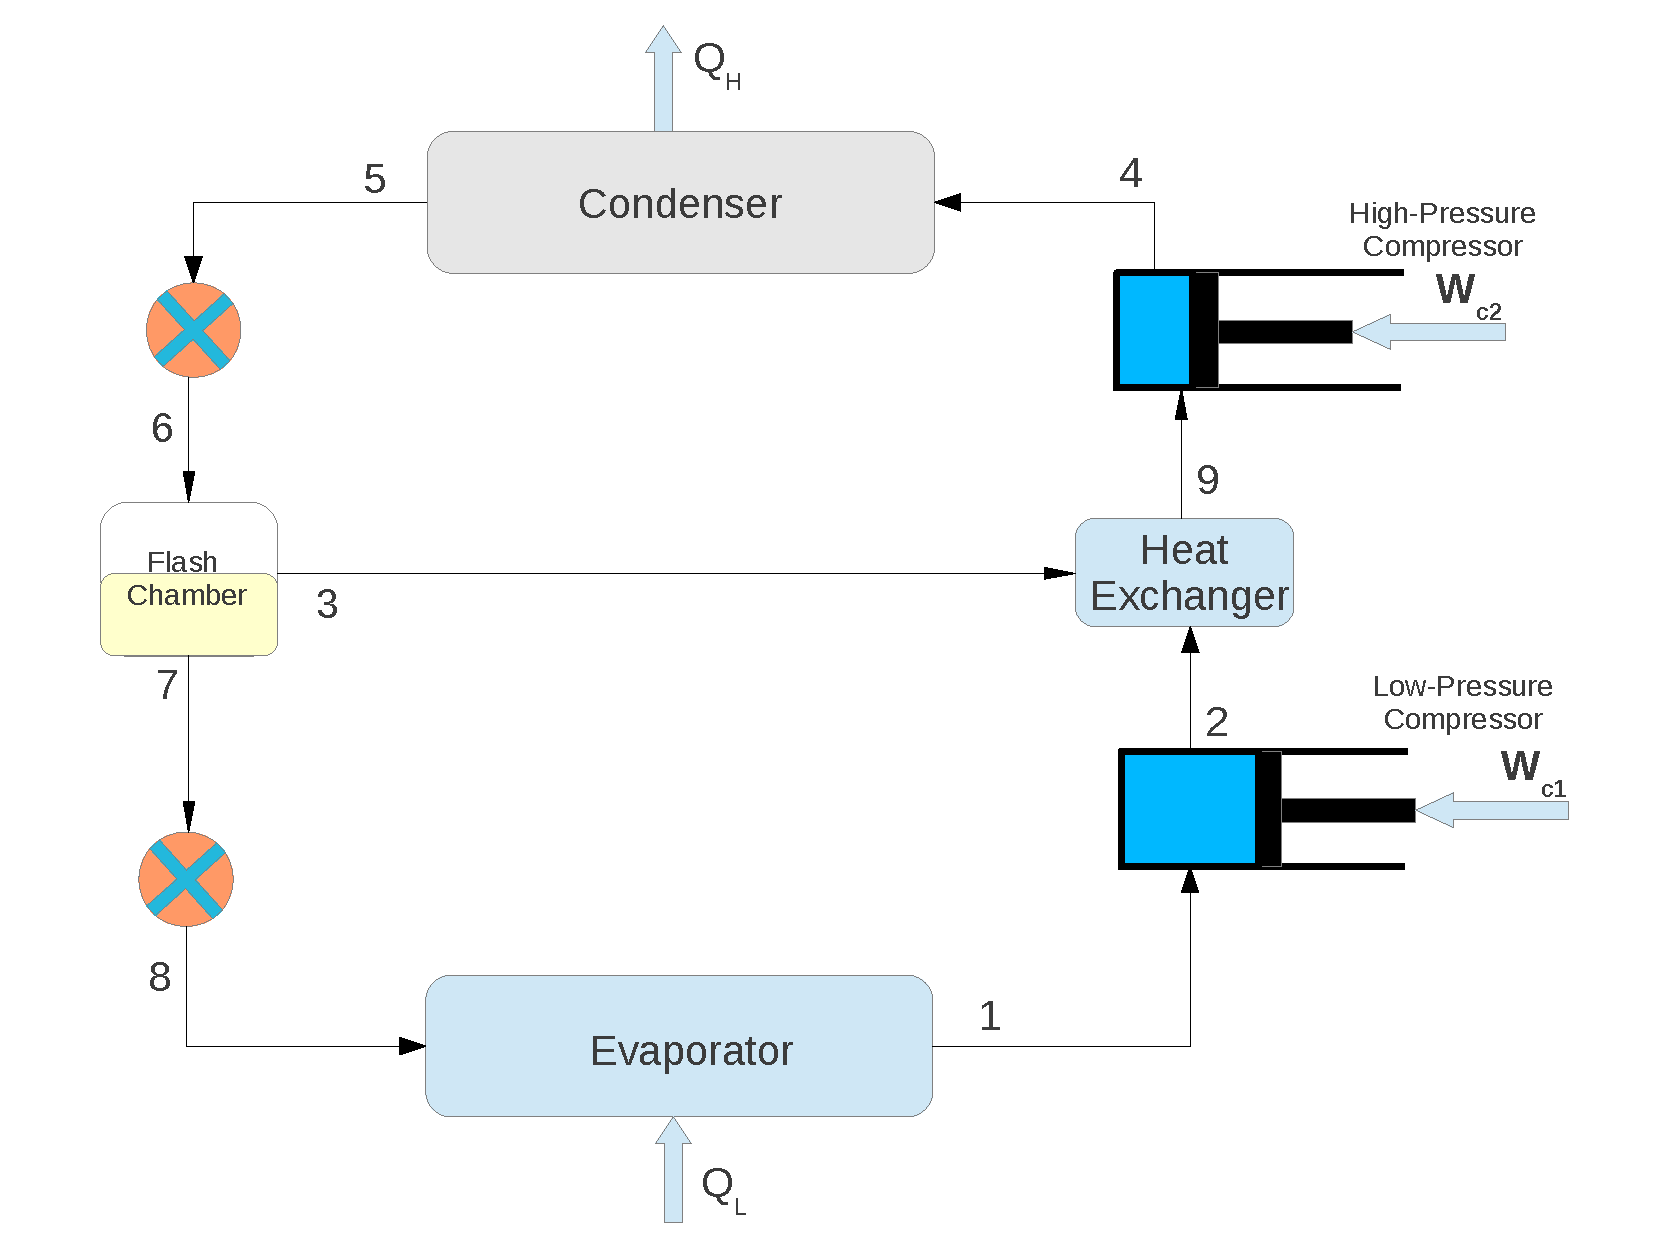
\includegraphics[width=4.5cm,height=3.5cm,clip]{./Pics/Overview_Refrig26}
      \vspace{-.1cm}
      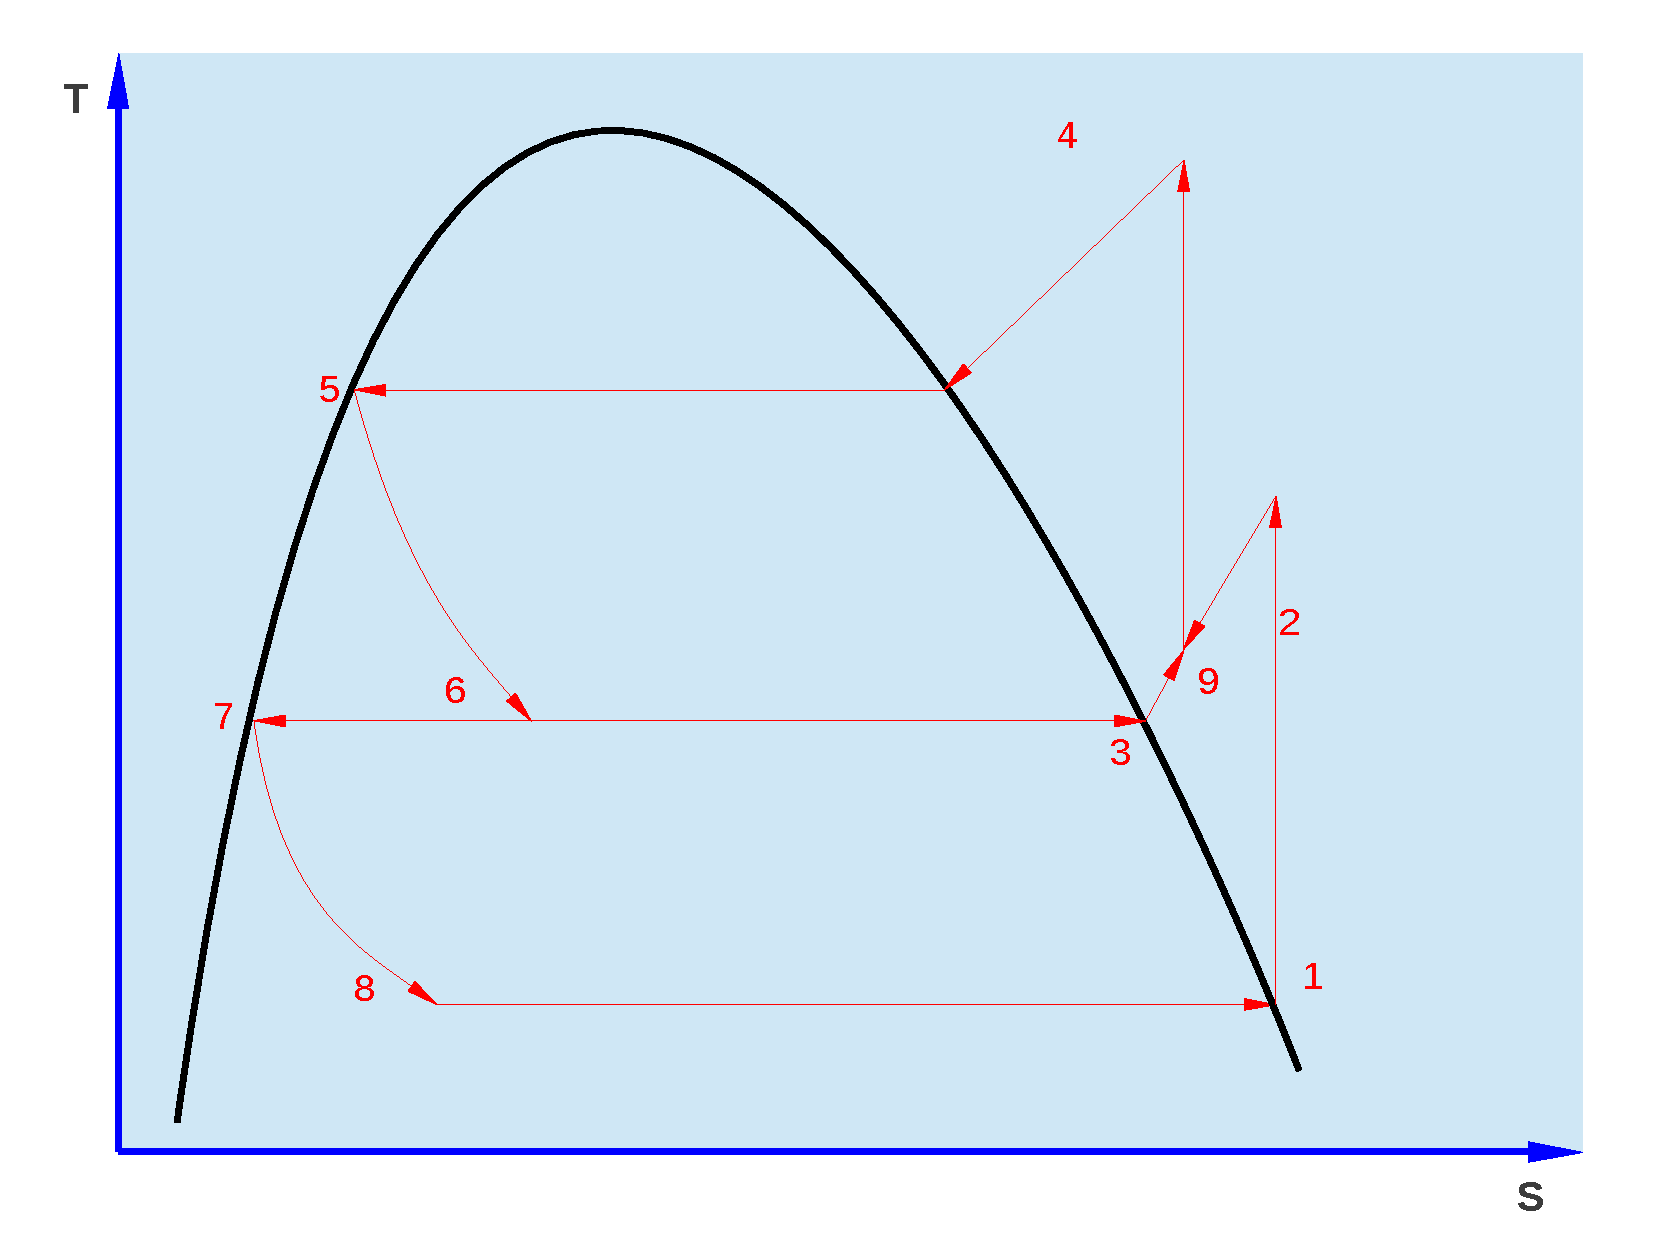
\includegraphics[width=4.cm,height=4.cm,clip]{./Pics/Overview_Refrig27}}
   \end{figure}  
  \end{column}  
  \begin{column}[c]{0.55\linewidth}
   \begin{enumerate}[(a)]\setcounter{enumi}{5}
    \item <1-> The fluid is then compressed in the HP (stage 4) and driven to the condenser where it becomes a saturated liquid;
    \item <2-> The liquid refrigerant is expanded (5-6) until the pressure is reduced to the interstage pressure and sent to the flash chamber;
    \item <3-> The liquid-vapour solution (2-phase region) from the condenser is separated (in the flash chamber) and;
    \item <4-> The liquid fraction is driven to the second expansion valve (7-8) where;
    \item <5-> The refrigerant pressure is reduced and the fluid is driven to the evaporator (8-1) where;
   \end{enumerate}
  \end{column}  
 \end{columns} 
\end{frame}


%%%
%%% Slide
%%%
\begin{frame}
 \frametitle{Multi-Stage Compression with Intercooling Refrigeration}
 \begin{columns}
  \begin{column}[c]{0.45\linewidth}
   \begin{figure}%
     \vbox{
      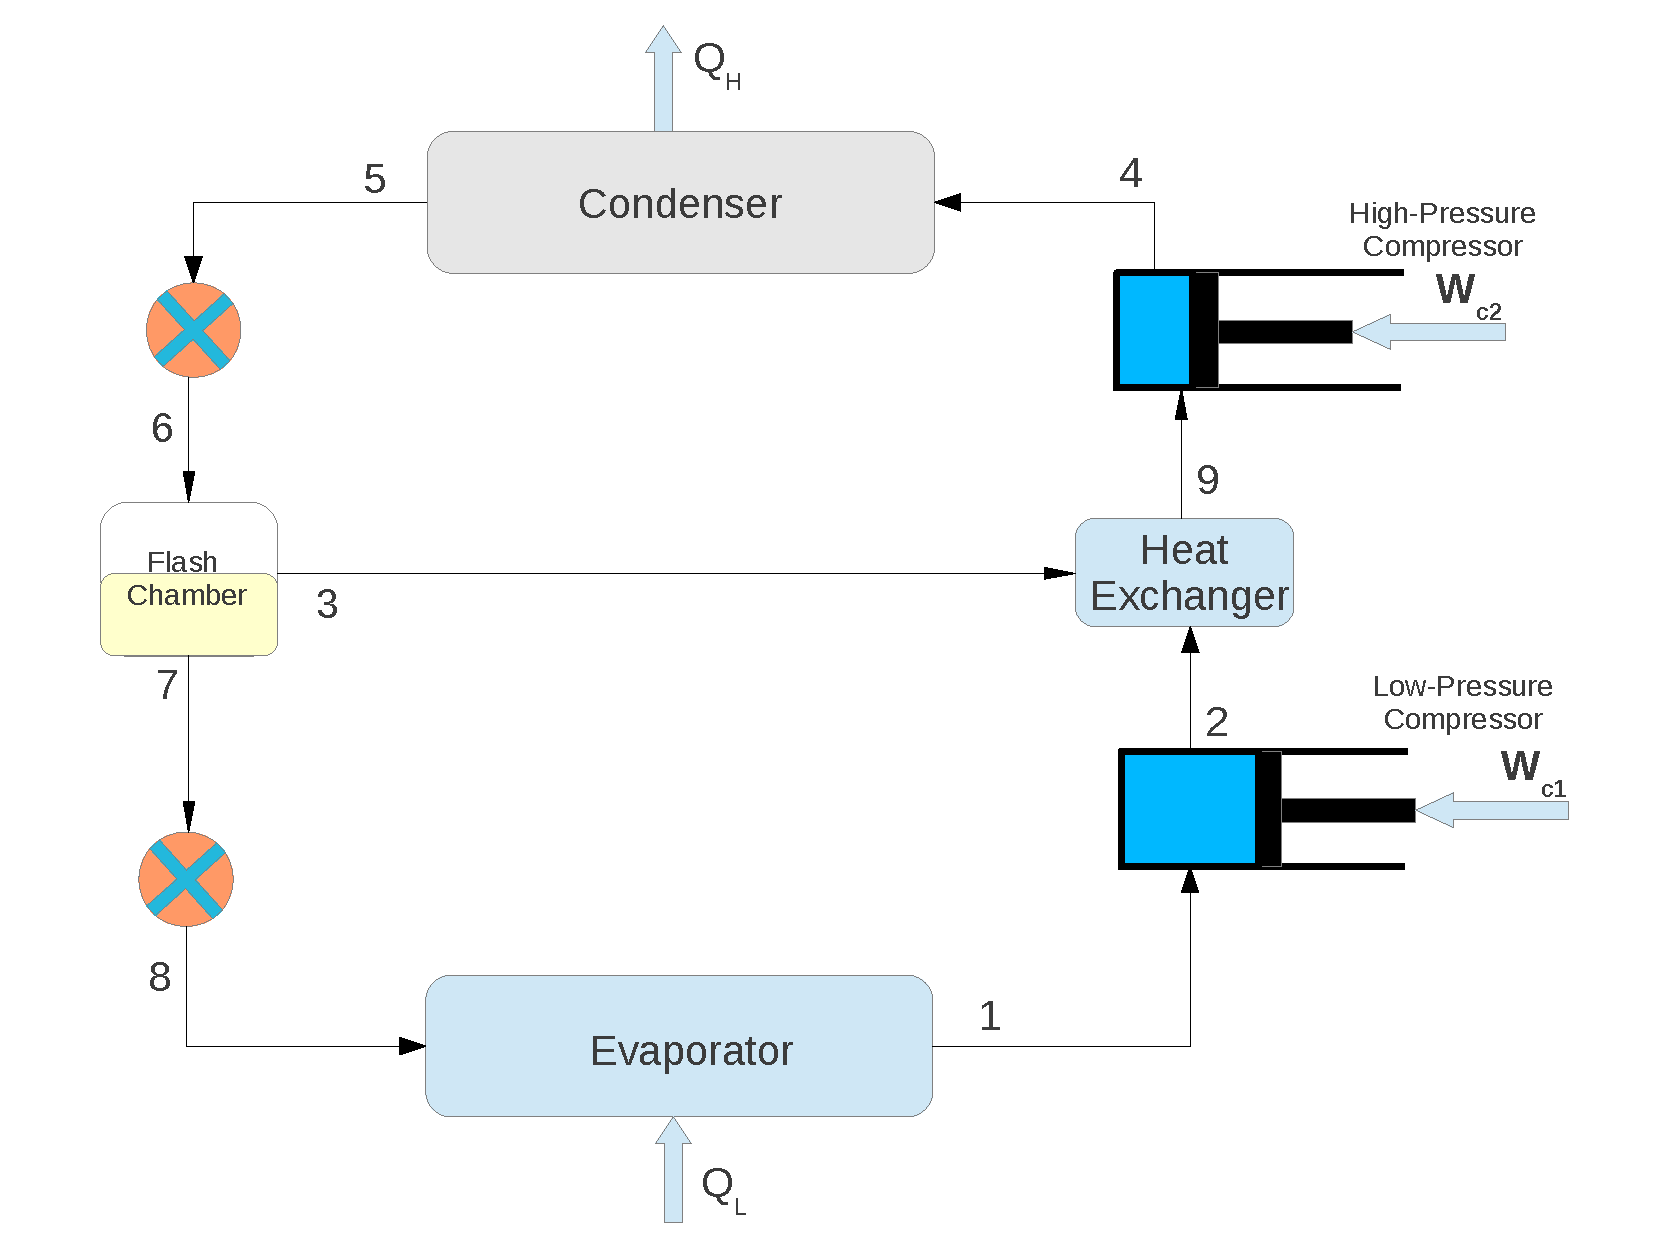
\includegraphics[width=4.5cm,height=3.5cm,clip]{./Pics/Overview_Refrig26}
      \vspace{-.1cm}
      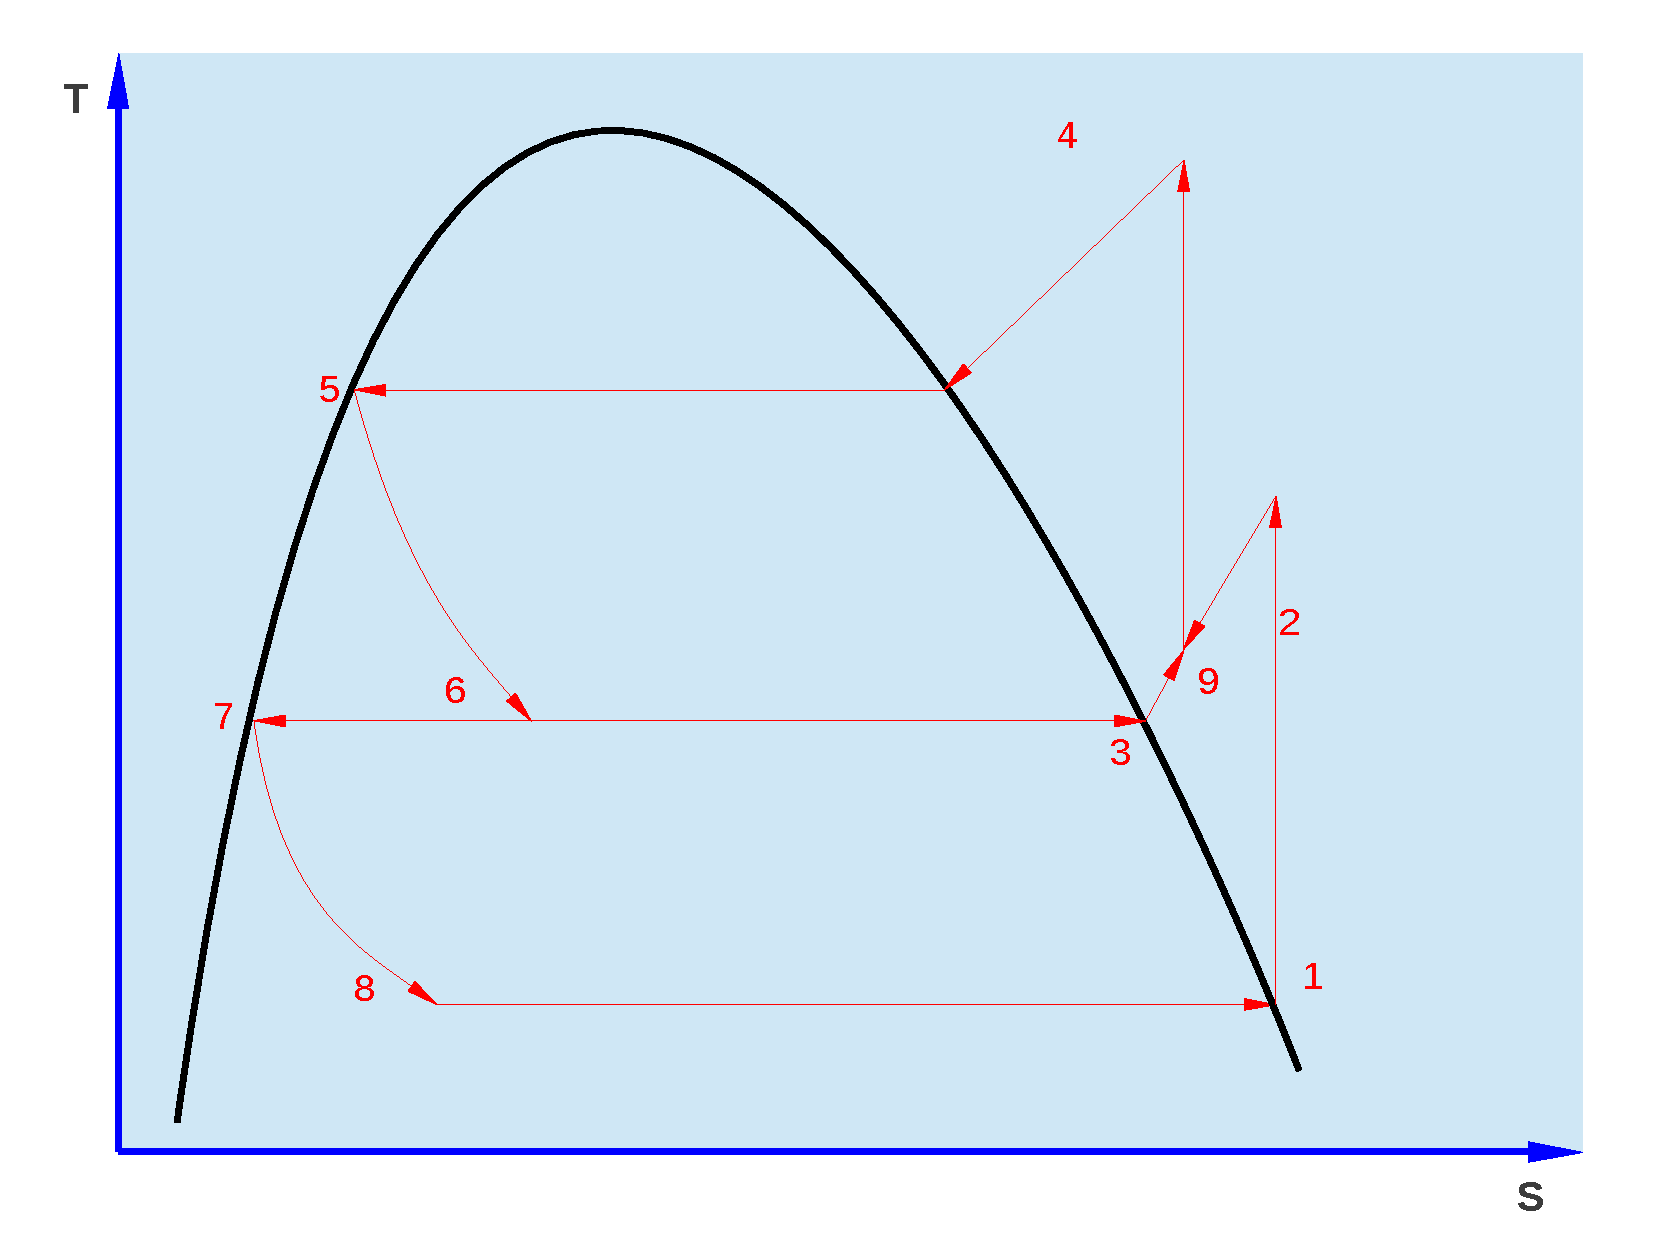
\includegraphics[width=4.cm,height=4.cm,clip]{./Pics/Overview_Refrig27}}
   \end{figure}  
  \end{column}  
  \begin{column}[c]{0.55\linewidth}
   \begin{enumerate}[(a)]\setcounter{enumi}{10}
    \item <1-> The liquid refrigerant is vaporised  by absorbing latent heat of vaporisation from the refrigerated space (cooling effect);
    \item <2-> The gas fraction (3) enters the heat exchange and is mixed with the fluid leaving the first LP compressor and driven to the HP compressor (9-4).
    \item <3-> For two-stage compression of a refrigerant with complete intercooling, for minimum work, the interstage pressure, $P_{i}$ is approximate to,
      \begin{displaymath}
       P_{i}=\sqrt{P_{1}P_{2}}
      \end{displaymath}
    \item <4-> Where $P_{1}$ is the suction pressure of the LP compressor and $P_{2}$ is the discharge pressure of the HP compressor.
   \end{enumerate}
  \end{column}  
 \end{columns} 
\end{frame}

%%%
%%% SECTION
%%%
\section{Heat Pumps}

\subsection{Overview}
%%%
%%% Slide
%%%
\begin{frame}
 \frametitle{Heat Pumps}
    \begin{figure}%
     \begin{center}
      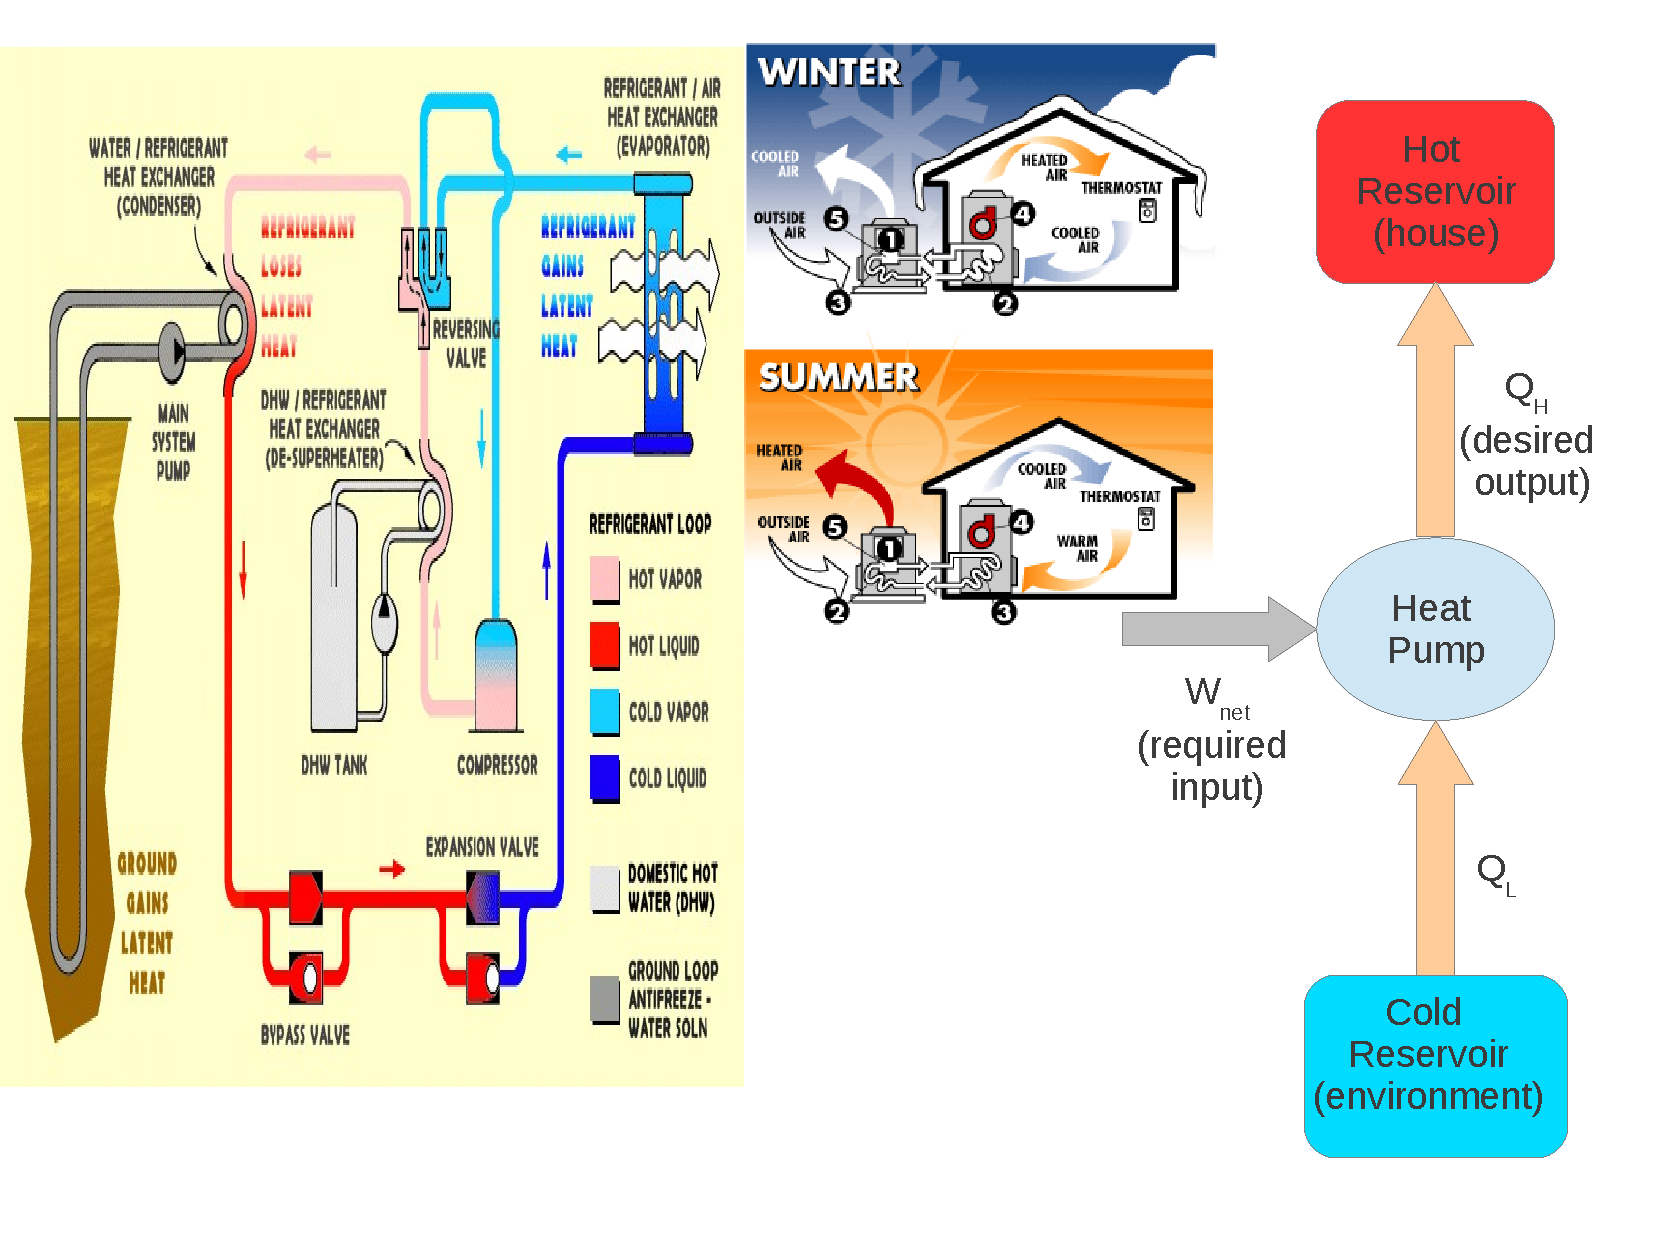
\includegraphics[width=12.cm,height=7.8cm]{./Pics/Overview_Refrig35}
     \end{center}
    \end{figure}
\end{frame}



%%% Slide
%%%
\begin{frame}
 \frametitle{Objectives}
  \begin{columns}
   \begin{column}[c]{0.45\linewidth}
  \begin{enumerate}[(i)]
   \item <1-> \textcolor{blue}{Heat Pumps} are devices that are used to \textcolor{blue}{maintain} a body at a temperature larger than the surroundings;
   \item <2-> They work in a very similar way as the refrigerators we have studied, but with \textcolor{red}{a difference} in the objective;
   \item <3-> \textcolor{blue}{HPs} keep the temperature of the body above to the temperature in the surroundings whereas;
   \item <4-> The \textcolor{blue}{refrigerators} maintain the temperature below the surrounding temperature.
  \end{enumerate}
   \end{column}
   \begin{column}[c]{0.55\linewidth}
    \begin{figure}%
     \begin{center}
      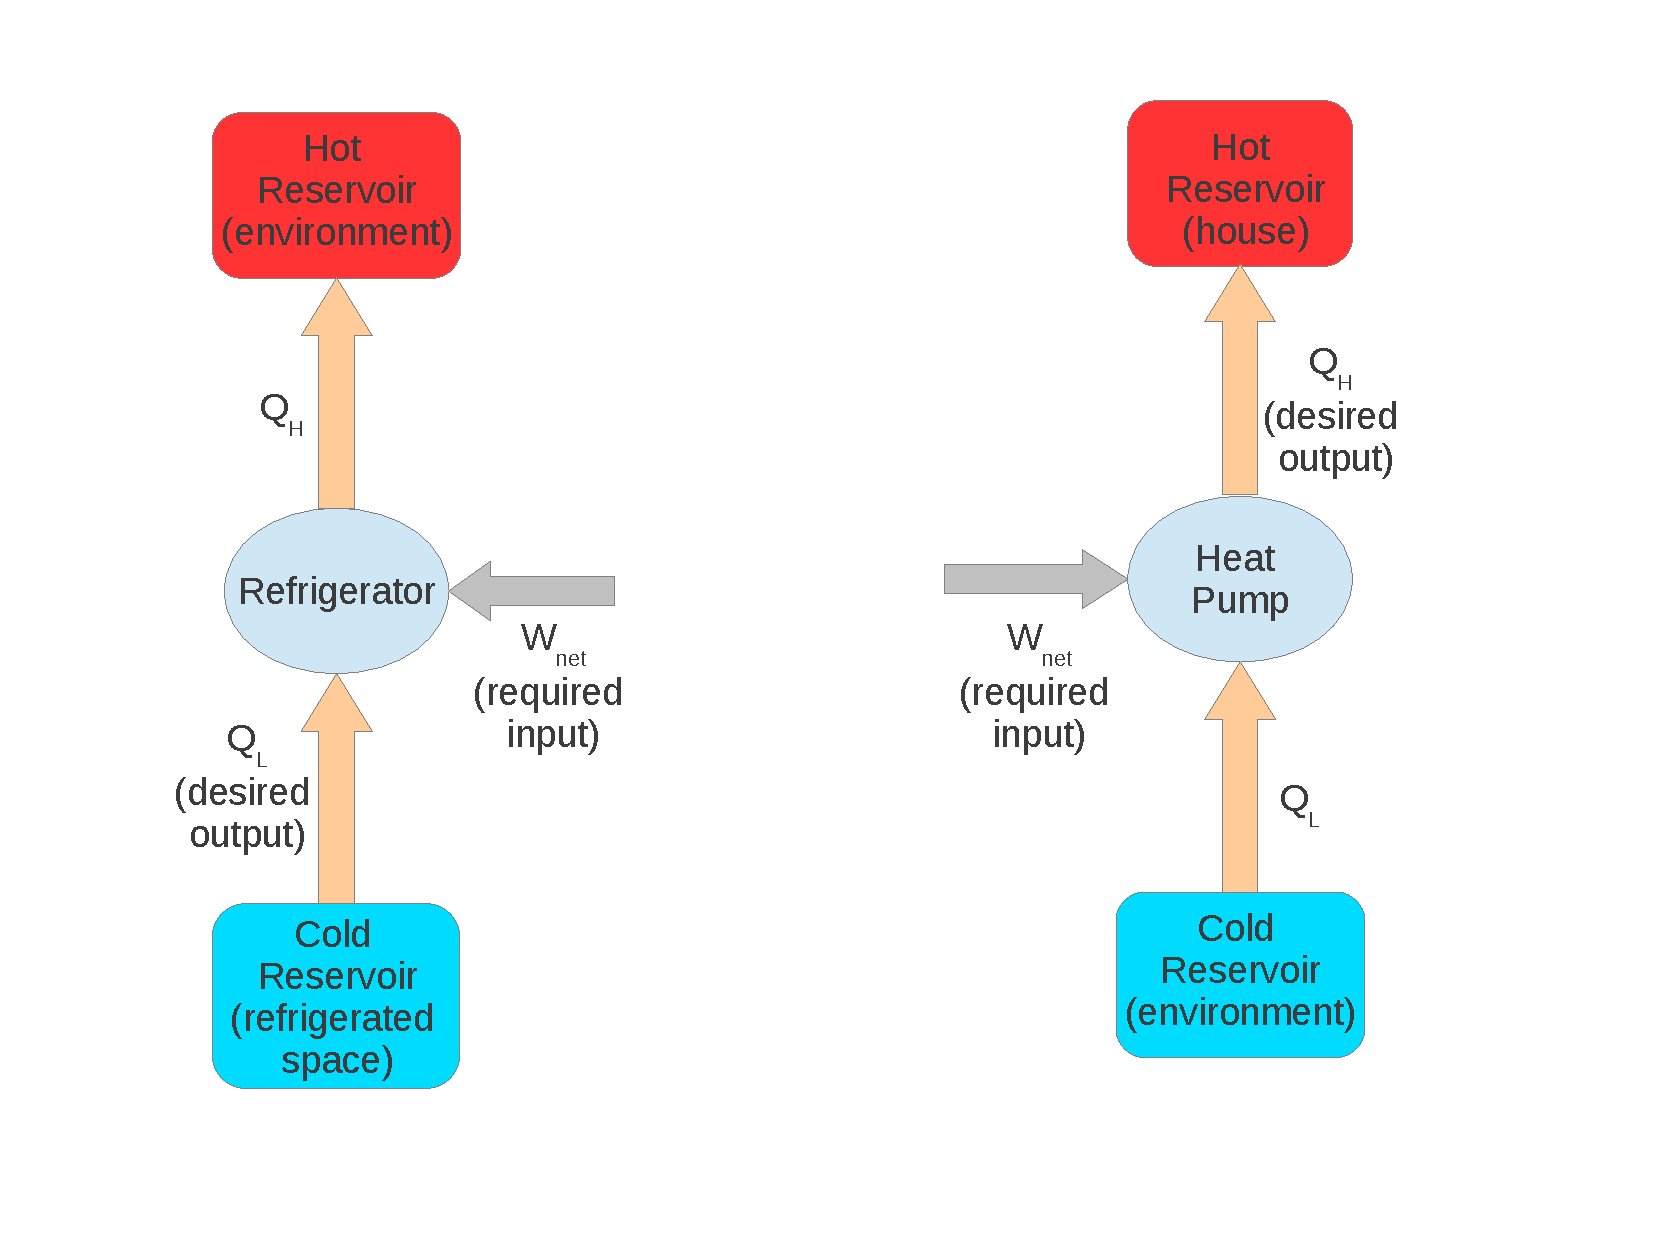
\includegraphics[width=7.5cm,clip]{./Pics/Overview_Refrig2}
     \end{center}
    \end{figure}  
   \end{column}  
  \end{columns}
\end{frame}


%%%
%%% Slide
%%%
\begin{frame}
 \frametitle{Objectives}
  \begin{columns}
   \begin{column}[c]{0.45\linewidth}
  \begin{enumerate}[(i)]
   \item <1-> \textcolor{blue}{HPs} can be based on vapour-compression cycle, absorption cycle, etc;
   \item <2-> \textcolor{blue}{Reversed Carnot cycle} is the thermodynamic cycle for \textcolor{blue}{HP};
   \item <3-> The figure in the rhs is a vapour-compression cycle representation of the heat pump;
   \item <4-> Where \textcolor{blue}{heat} is removed in the \textcolor{blue}{condenser}.
  \end{enumerate}
   \end{column}
   \begin{column}[c]{0.55\linewidth}\vspace{-1.cm}
    \begin{figure}%
     \begin{center}
      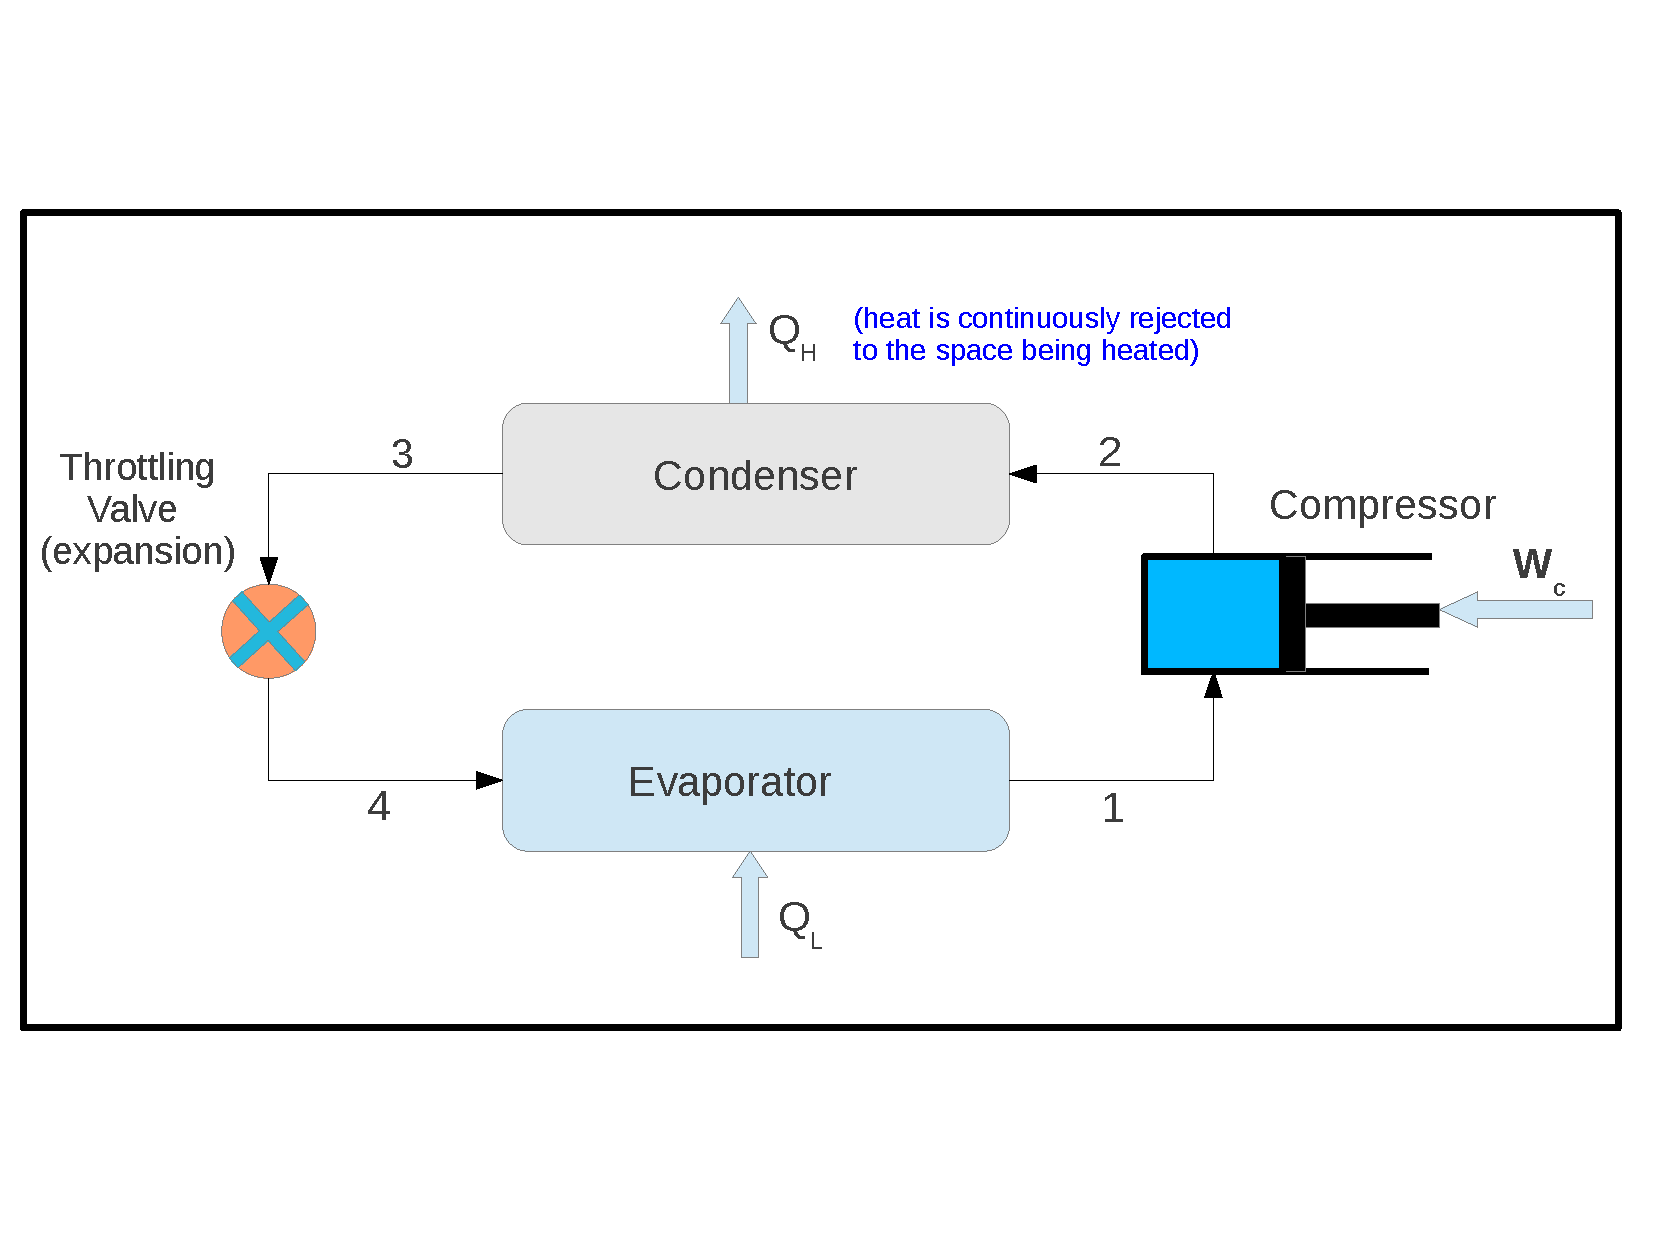
\includegraphics[width=6.5cm,clip]{./Pics/Overview_Refrig36}
     \end{center}
    \end{figure}  
   \end{column}  
  \end{columns}
\end{frame}


\subsection{COP in HPs}
%%%
%%% Slide
%%%
\begin{frame}
 \frametitle{Coefficient of Performance in HPs}
    \begin{figure}%
     \begin{center}
      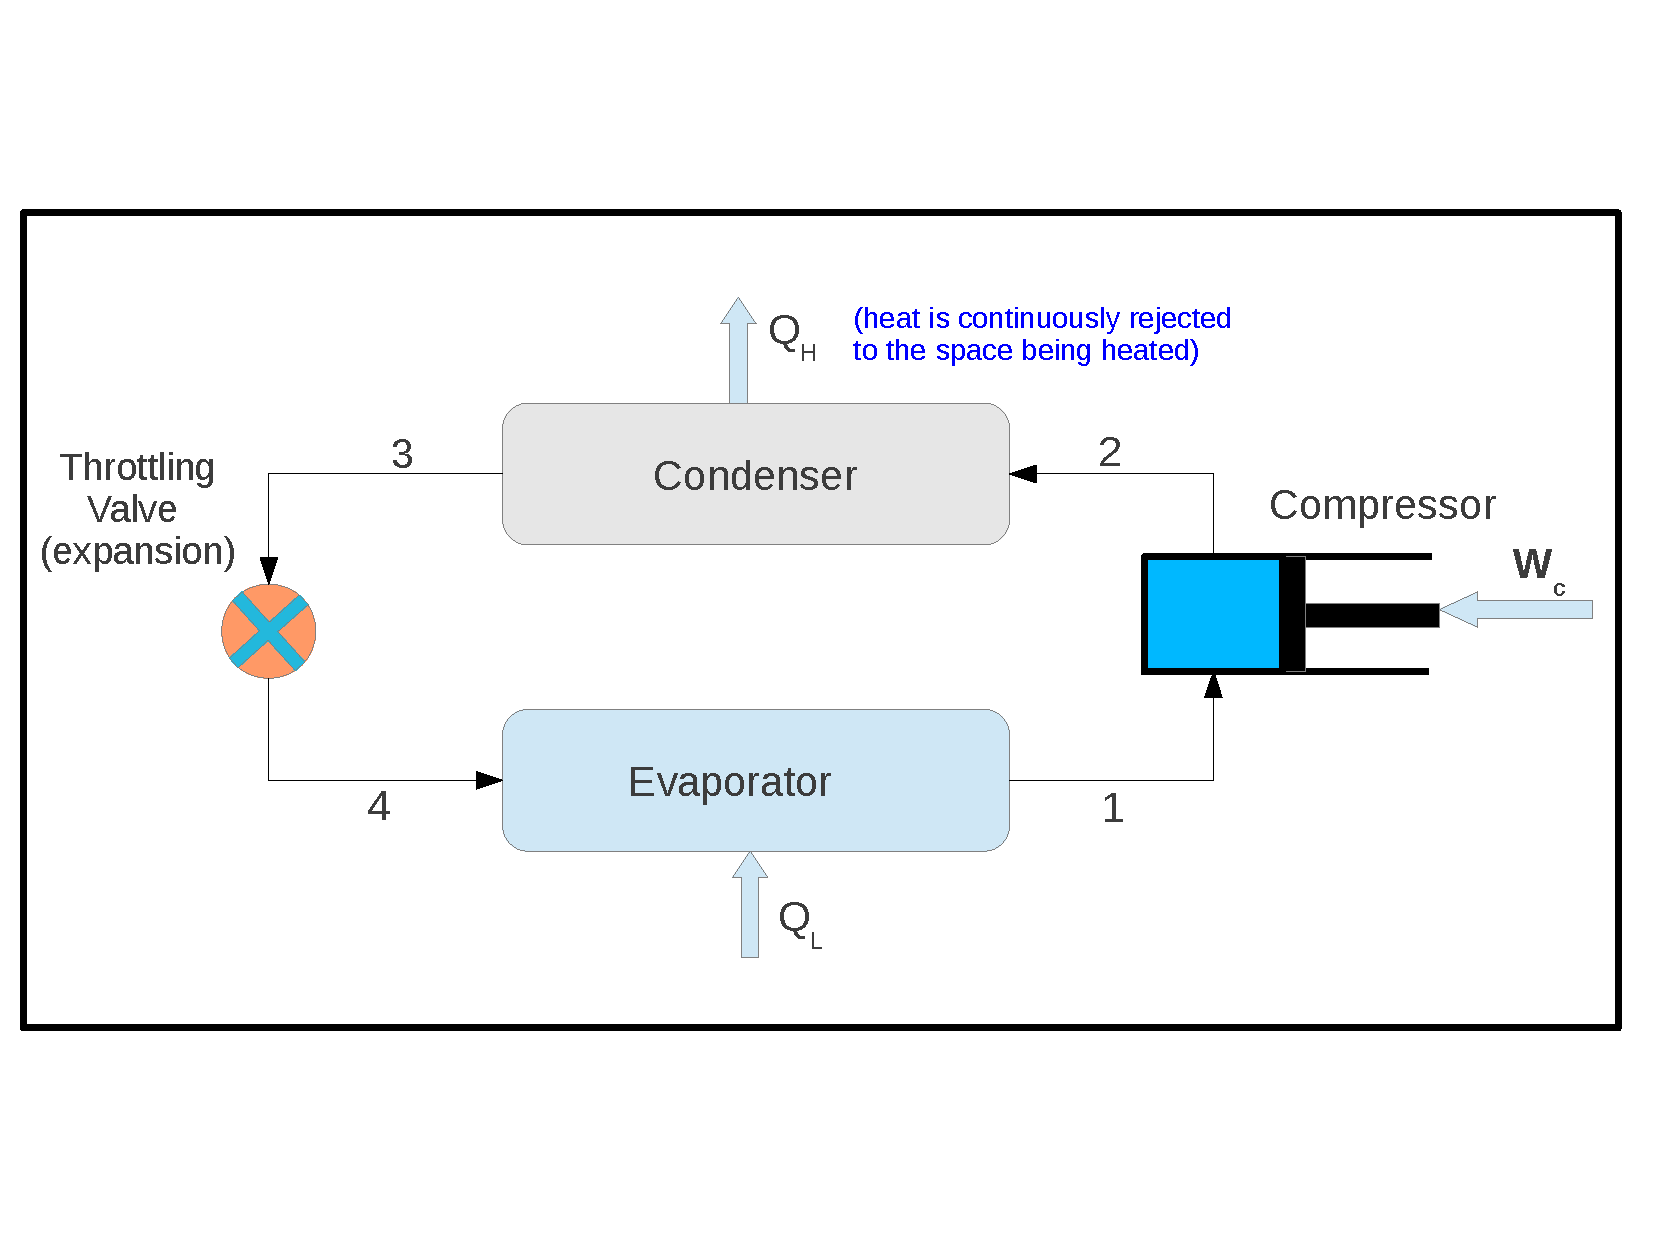
\includegraphics[width=6.5cm,clip]{./Pics/Overview_Refrig36}
     \end{center}
    \end{figure} 


  \begin{enumerate}[(i)]
   \item <1-> The \textcolor{blue}{Coefficient of Performance} is given by
    \begin{displaymath}
     \textcolor{blue}{\text{COP}} = \frc{\text{Desired Effect (heating of space)}}{\text{Net Work}} = \frc{m\left(H_{3}-H_{2}\right)}{m\left(H_{2}-H_{1}\right)} = \textcolor{blue}{\frc{H_{3}-H_{2}}{H_{2}-H_{1}}}
    \end{displaymath}
   \item <2-> \textcolor{blue}{COP of Heat Pumps} usually range from 1.5 and 4.
  \end{enumerate}
\end{frame}


\section{Summary}
%%%
%%% Slide
%%%
\begin{frame}
 \frametitle{Summary}
  \begin{itemize}
   \item <1-> Components of refrigerant cycles;
   \item <2-> Coefficient of Performance;
   \item <3-> Refrigerants and Heat Pumps operate in the same way but with different objectives;
   \item <4-> The focal point in \textcolor{blue}{refrigerators} is the \textcolor{red}{heat absorbed from the Evaporator}, whereas;
   \item <5-> In \textcolor{blue}{heat pumps}, \textcolor{red}{heat is released in the Condenser}.
  \end{itemize}
\end{frame}



\end{document}
